\documentclass[12pt]{article}
\usepackage[utf8]{inputenc}
\usepackage[dvipsnames]{xcolor}
\usepackage[leqno]{amsmath}
\usepackage{amssymb}
%\usepackage{units}
\usepackage{wallpaper}
\usepackage{newtons-notebook}
\usepackage{booktabs}
\usepackage{float}
\usepackage{xurl}
\usepackage{listings}
%\usepackage{tocloft}
\usepackage{amsmath}
\usepackage{amsthm}
\usepackage{amsfonts}
\usepackage{amssymb}

\usepackage{tabu}
%\usepackage{multirow}
\usepackage{array}

\usepackage[english]{babel}
\usepackage{longtable}
%\usepackage[table]{xcolor} 
%\usepackage{indentfirst}

%\usepackage{gensymb}

\usepackage{hyperref}
\usepackage{color}
\usepackage[table,xcdraw]{xcolor}

\usepackage[font=small,skip=0pt]{caption}

\usepackage{graphicx}
\graphicspath{ {./assets/} }

\usepackage{setspace}
\usepackage{titlesec}

\usepackage{wrapfig}

% https://tex.stackexchange.com/questions/19660/how-to-make-the-size-of-pdf-output-wider
\setlength{\paperwidth}{8.75in} % set dimension of \paperwidth to add .125 inch on either sidev
\addtolength{\paperheight}{0.25in} % enlarge \paperheight by .25 inch

\titlespacing\section{0pt}{12pt plus 4pt minus 2pt}{0pt}
\titlespacing\subsection{0pt}{12pt plus 4pt minus 2pt}{0pt}
\titlespacing\subsubsection{0pt}{12pt plus 4pt minus 2pt}{0pt}

%\renewcommand{\cftpartfont}{\Large\bfseries}
%\renewcommand{\cftsecfont}{\normalsize}

% deals with space between paragraphs
\setlength{\parskip}{\baselineskip}
\renewcommand{\baselinestretch}{1.4}

% Margin Formatting https://en.wikibooks.org/wiki/LaTeX/Page_Layout
\addtolength{\hoffset}{0in}
\addtolength{\voffset}{0in}
\addtolength{\oddsidemargin}{-.125in}
\addtolength{\textwidth}{0.5in}
\addtolength{\topmargin}{-.125in}

% Theorem Enumeration https://tex.stackexchange.com/questions/371731/versioning-theorem-numbers-with-amsthm
\newcounter{dfnmain}[section]
\newtheorem{dfninner}{Definition}[dfnmain]
\makeatletter
\renewcommand{\thedfninner}{%
  \arabic{dfnmain}.\@arabic{\numexpr\value{dfninner}-1\relax}%
}
\makeatother
\newenvironment{dfn}
 {\stepcounter{dfnmain}\dfninner}
 {\enddfninner}
\newenvironment{dfn*}
 {\dfninner}
 {\enddfninner}
 
% Example formatting https://tex.stackexchange.com/questions/357810/math-example-formatting
\newenvironment{exm}[1]{%
  \par  % start a new paragraph
  \bigskip  % insert some vertical whitespace
  \noindent % no paragraph indentation
  \textbf{Example #1}}{%
  \par%\bigskip % insert another paragraph break and more vert. whitespace
}

\usepackage{tikz}

\newtheorem{theorem}{Theorem}

\theoremstyle{definition}
\newtheorem{definition}{Definition}

\newtheorem{problem}{Problem}

\newtheorem*{solution}{Solution}

\newtheorem*{remark}{Remark}

\newtheorem{assumption}{Assumption}

\begin{document}
\setcounter{tocdepth}{1}

% v COMMENT THIS OUT BEFORE SENDING THE FINAL VERSION TO PRINT, THEY DON'T WANT THE COVERS
% \nnimagepage{2021_Front_Cover.pdf}

\nnwallpaper{2021_Intro_Section_Page_Border.pdf}

\begin{figure}[H]
    \centering \includegraphics[scale=.9]{newton.jpg}
\end{figure}

\begin{center}
    \textit{To explain all nature is too difficult a task\\
    for any one man or even for any one age.\\
    'Tis much better to do a little with certainty\\
    and leave the rest for others that come after you.}\\
    	$\sim$Isaac Newton
\end{center}

\newpage
\begin{spacing}{1}
\tableofcontents
\end{spacing}

%\begin{figure}[H]
%    \centering
%    \vspace*{75pt}
%    \includegraphics[scale=1.25]{newtons_notebook_fibonacci_spiral.png}
%\end{figure}

\newpage
\subsection*{Mission Statement}
\textit{Newton’s Notebook: The Haverford School STEM Journal} is designed to enhance the interests, talents, and achievements of individuals in mathematics and science and to promote the work of those most passionate about these disciplines. The following articles were written by members and friends of the Haverford community and edited by the \textit{Notebook} staff. We hope these articles inspire readers to further discover the universally beautiful realm of STEM exploration. 
\subsection*{Staff}
{\centering{}
    \textbf{Editors-in-Chief:} Gary Gao '21, Mitav Nayak '22
    \\
    \textbf{Designer-in-Chief:} Mitav Nayak '22
    \\ 
    \textbf{Assistant Editors:} Brian Williams '21, Adamya Aggarwal '22
    \\
    \textbf{Faculty Advisor:} Dr.\ Mark Gottlieb
    \\}
\subsection*{Featured Polymath: John Forbes Nash Jr. (1928-2015)}
John Forbes Nash Jr. was an American mathematician best known for his work in game theory, partial differential equations, cryptography, and mathematical economics. While attending high school in Bluefield, West Virginia, he also enrolled in courses in advanced mathematics at a local community college. Nash went on the graduate with a bachelor’s degree and master’s degree in mathematics from the Carnegie Institute of Technology—now Carnegie Mellon University—when he was just 19 years old. He then attended Princeton University on a scholarship for graduate school and obtained a PhD with a dissertation in non-cooperative games in 1950, at 22 years of age. In his dissertation, he included the foundations for what later came to be known as the Nash equilibrium, which won him the John von Neumann Theory Prize in 1978, the Nobel Prize in Economic Sciences in 1994, and the Leroy P. Steel Prize in 1999. During much of his life, Nash suffered from mental illness. He joined the Massachusetts Institute of Technology in 1951 to research partial differential equations and teach mathematics, but he resigned in 1959 as a result of his schizophrenia and was admitted to a number of hospitals during the 1960s. In 1970, he was discharged from the hospital for the last time, and eventually returned to Princeton as a senior research mathematician. Nash’s extraordinary life is portrayed in the Academy Award-winning film \emph{A Beautiful Mind} (2001).
\newpage

% Begin the pure math section
\addcontentsline{toc}{part}{Pure Mathematics}
\nnimagepage{2021_Pure_Math_Section_Title.pdf}

\nnwallpaper{2021_Pure_Math_Page_Border.pdf}
\def\currentTitleWallpaper{2021_Pure_Math_Title_Page_Border.pdf}

\nnarticleheader{An Interesting Example of the Use of Checksum}{Gary Gao, Haverford '21}

\noindent
\textbf{A Story}

	In an ancient kingdom, there was a tyrant king. One day, he caught two people who turned out to be magicians. The tyrant king wanted to kill them, but he magicians magically persuaded the king to agree to play a game with them. The king said, ``Tomorrow, I will have two hats ready. Each of them can be blue or red. I will have you sit down and face each other, and then put one hat on each of your heads, so you will only be able to see the color of the hat on the other person's head. After that, you will guess the color of the hat on your own head and you will say it out at the same time. If any of you two can guess correctly, I will let you go. Otherwise, you will die." The magicians agreed, and they have a night to discuss a strategy to increase their chances of winning. Is there a way for them to save themselves for sure?\\
	\indent In fact, the strategy for them is quite simple. They can do the following: Magician 1 will say the color that is the same color as what he sees. Magician 2 will say the color that is different from what he sees. Because they have actually split the the 4 possibilities into two cases: Magician 1 bet that the color of their hats are the same; Magician 2 bet that the color of their hats are different. In this way, exactly one of them will guess correctly. Thus, they are saved.

\noindent
\textbf{A Generalization}

	After seeing this story, we can try to solve this problem.
	\begin{problem}
		10 people stand on a circle. Each person has a hat on the head. Each hat can be any of the 10 given colors. Every person can see the hat on the head of all other people but not himself. They will guess the color of the hat on their own head. They will say their guesses out loud at the same time, but they are allowed to discuss strategy in advance. Can you guarantee that one of them will guess correctly?
	\end{problem}
	\begin{solution}	
		We number the color with the integers from 0 to 9 and number the 10 people with the integers from 0 to 9 clockwise. Define $a_i$ to be the number corresponding to the color of the hat on the head of the $i$th person. And the strategy will be the following: Person $j$ will assume that $a_0+a_1+...+a_9 \equiv j \mod 10$ and calculate $a_k$ based on the color of other people's hats and $j$. In this way, the $k$th person will guess correctly, where $a_0+a_1+...+a_9 \equiv k \mod 10$, when calculated with the actual values.
	\end{solution}
	This is related to the concept of checksums, because in the strategy, every person's guess depends on this expression $(a_0+a_1+...+a_9)\mod 10$.

\noindent	
\textbf{Further Generalization}

	Now that we have figured out the structure of this type of problems, we can aim for a more generalized, optimal conclusion.
	\begin{problem}
		$n$ people stand on a circle. Each person has a hat on the head. Each hat can be any of the $c$ given colors. Every person can see the hat on the head of all other people but not himself. They will guess the color of the hat on their own head. They will say their guesses out loud at the same time, but they are allowed to discuss strategy in advance. At most how many people can guess correctly for sure?
	\end{problem}
	\begin{solution}
		Similar to our solution to problem 1, we can number the color with the integers from 0 to $c-1$. We will number the n people with the integers from 0 to $n-1$ clockwise. Define $a_i$  to be the number corresponding to the color of the hat on the head of the $i$th person. \\
		The strategy will be the following: Person $j$ will assume that $a_0+a_1+...+a_{n-1} \equiv j \mod c$ and calculate $a_k$ based on the color of other people's hats and $j$. In this way, the $k$th person will guess correctly if $a_0+a_1+...+a_{n-1} \equiv k \mod c$ when calculated with the actual values. It is easy to see that the amount of people that is guaranteed to guess correctly is equal to $\lfloor \frac{n}{c} \rfloor$\\
		We also want to prove that $\lfloor \frac{n}{c} \rfloor$ is the maximum. We can notice that among all the possible $c^n$ possibilities, each specific person can guess correctly $c^{n-1}$ times. This means the expected value of correct guesses from each person each time is $\frac{c^n}{c^{n-1}} = \frac{1}{c}$. By the linearity of expectation, the expected number of correct guesses each time is $n \cdot \frac{1}{c} = \frac{n}{c}$, which means there exist at least one situation where at most $\lfloor \frac{n}{c} \rfloor$ guesses correctly. So $\lfloor \frac{n}{c} \rfloor$ is the maximum amount we want.
	\end{solution}
	\indent We can see that checksums are very powerful in finding strategies for this kind of problems. For problems with more restrictions, it is also possible that we use more sophisticated checksum that can involve polynomial and more modular expressions.


\newpage

\nnarticleheader{Random Variables}{Adamya Aggarwal, Haverford '22}

\section*{Random Variables}
In experiments, we are sometimes more interested in some value associated with an event as opposed to the actual event itself. Consider an experiment that flips a coin 5 times. We may not actually care that the order is TTHTH, but we do care about the number of heads that occur (in this case, 2). These values of interest are called random variables.

\begin{definition}
    A discrete random variable $X$ on a sample space $\Omega$ is a function that assigns each sample point $\omega \in \Omega$ a real value $X(\omega)$.
\end{definition}

Note: $\Omega$ is the set of all possible outcomes of an experiment, and $\omega$ is one such outcome.

\vspace{2.5mm}

For a random variable $X$ and a real value $j$, the event $X = j$ is the set of outcomes in $\Omega$ for which $X$ assumes the value $j$. That is, 
\[
X = j \equiv \{\omega \in \Omega | X(\omega) = j \}
\]

\begin{definition}
    An indicator/dummy/binary/Bernoulli variable (there are many names for it) is a random variable that only takes the value 0 or 1.
\end{definition}

\begin{definition}
    The probability mass function (PMF), denoted by $p_{X}$, gives the probability that a random variable $X$ is exactly equal to some value $x$. It can be represented mathematically as follows:
    \[
    p_{X}(x) = \Pr[X = x]
    \]
\end{definition}

Note that 
\[
\sum_{x} p_{X}(x) = \sum_{x} \Pr[X = x] = 1
\]
This is because the events $X = x$ are disjoint and thus partition the sample space $\Omega$. (Going back to the 5 coin flip example, this is logical because for example, there cannot be both 2 and 3 heads in any given sequence.)

\begin{definition}
    Two random variables X and Y are independent if and only if
    \[
    \Pr[X = x \cap Y = y] = \Pr[X = x] \times \Pr[Y = y]
    \]
\end{definition}

Simply put, X and Y are independent if the occurrence of one does not affect the probability of occurrence of the other.

\section*{Expectation}

\begin{definition}
    The expected value of a random variable $X$ is a weighted average of the possible values that X can take. The expectation is what you would expect the outcome of an experiment to be on average.
    \[
    \E[X] = \sum_{x} x p_{X}(x) = \sum_{x} x \Pr[X = x]
    \]
\end{definition}
Note: The expected value of an indicator variable $X_{i}$ is just $\Pr[X_{i} = 1]$.

\vspace{5mm}

\textbf{Example 1:}
In the running example of 5 coin flips, find the expectation of the number of heads.

\vspace{2.5mm}

\textbf{Solution:}
\begin{align*}
\begin{split}
    \E[X] ={}& 0 \times \Pr[X = 0] + 1 \times \Pr[X = 1] + 2 \times \Pr[X = 2] + 3 \times \Pr[X = 3]\\
    & + 4 \times \Pr[X = 4] + 5 \times \Pr[X = 5]
\end{split}\\
    ={}& 0 \times \frac{1}{32} + 1 \times \frac{5}{32} + 2 \times \frac{10}{32} + 3 \times \frac{10}{32} + 4 \times \frac{5}{32} + 5 \times \frac{1}{32} \\
    ={}& 0 + \frac{5}{32} + \frac{20}{32} + \frac{30}{32} + \frac{20}{32} + \frac{5}{32} \\
    ={}& \frac{80}{32} \\
    ={}& 2.5
\end{align*}

Thus, the expected value for the number of heads in any given 5 flips is 2.5. Note that the expectation of a random variable does not necessarily have to be a valid value of the random variable (i.e. there can never actually be 2.5 heads). Think of it this way: if we were to run this experiment an infinite number of times, the average number of heads for all of those experiments would tend toward 2.5.

\vspace{5mm}

\textbf{Example 2:}
If you rolled two dice, in expectation, what is the sum?

\vspace{2.5mm}

\textbf{Solution:} \\
Let S be a random variable that denotes the sum of the roll of the 2 dice.

$$
\Pr[S = s] = 
\begin{cases}
\frac{1}{36} & \text{if $s$ = 2 or 12}\\
\frac{2}{36} & \text{if $s$ = 3 or 11}\\
\frac{3}{36} & \text{if $s$ = 4 or 10}\\
\frac{4}{36} & \text{if $s$ = 5 or 9}\\
\frac{5}{36} & \text{if $s$ = 6 or 8}\\
\frac{6}{36} & \text{if $s$ = 7}\\
\end{cases}
$$

To find the expectation, we can do the following calculations:
\begin{align*}
    \E[X] ={}& \sum_{x=2}^{12} x \Pr[X = x] \\
    \begin{split}
        ={}& (2 + 12) \times \frac{1}{36} + (3 + 11) \times \frac{2}{36} + (4 + 10) \times \frac{3}{36} + (5 + 9) \times \frac{4}{36} \\
        & + (6 + 8) \times \frac{5}{36} + (7) \times \frac{6}{36}
    \end{split} \\
    ={}& 7
\end{align*}

The expected value for the sum of the two dice is 7.

\subsection*{Linearity of Expectation}
Linearity of expectation is the property that the expected value of the sum of random variables is equal to the sum of their individual expected values, regardless of whether they are independent.
\begin{theorem}
    If $X = X_{1} + X_{2} + \ldots + X_{n}, then \E[X] = \E[X_{1}] + \E[X_{2}] + \ldots + \E[X_{n}]$. That is,
    \[
    \E[\sum_{i=1}^{n} X_{i}] = \sum_{i=1}^{n} E[X_{i}]
    \]
\end{theorem}
From linearity of expectation, we can further deduce that E[cX] = cE[X].

\vspace{5mm}

\textbf{Example 3:}
Use linearity of expectation to find the expected sum of 2 dice.

\vspace{2.5mm}

\textbf{Solution:} \\
We still want to find $\E[X]$, but there is another way to arrive at the solution. Let $X_{1}$ and $X_{2}$ be random variables denoting the results of the first and second rolls, respectively. Realize that because $X = X_{1} + X_{2}$,
    $$
    \E[X] = \E[X_{1} + X_{2}]
    $$
    
Using linearity of expectation, we get
    \begin{align*}
        \E[X] &= \E[X_{1}] + \E[X_{2}] \\
        &= \frac{1}{6}(1 + 2 + 3 + 4 + 5 + 6) + \frac{1}{6} (1 + 2 + 3 + 4 + 5 + 6) \\
        &= 7
    \end{align*}
    
\subsection*{The Hat Check Problem}
Suppose n people check in their hats at a hat check. The hats are returned randomly. In expectation, what is the number of people that get their own hat back?

\vspace{2.5mm}

\textbf{Solution:} \\
Let X be a random variable denoting the number of people who get their own hat back. Remember,
    $$
    \E[X] = \sum_{x=0}^{n}x\Pr[X = x]
    $$
But how can we calculate the probability of $x$ people getting their hats back? Let’s use indicator variables to make the problem more manageable. Let $X_{i}$ be an indicator variable that equals 1 if the $i^{\text{th}}$ person gets their hat back and equals 0 otherwise. Then,
    \begin{align*}
        X &= \sum_{i=1}^{n}X_{i} \\
        \E[X] &= \E[\sum_{i=1}^{n}X_{i}]
    \end{align*}
By linearity of expectation,
    $$
    \E[X] = \sum_{i=1}^{n}\E[X_{i}]
    $$
Because $X_{i}$ can only equal 0 or 1, we can rewrite this as
    \begin{align*}
        \E[X] &= \sum_{i=1}^{n}(0 \times \Pr[X_{i} = 0] + 1 \times \Pr[X_{i} = 1]) \\
        &= \sum_{i=1}^{n}\Pr[X_{i} = 1]
    \end{align*}
Notice that $X_{i}$ and $X_{j}$ are not independent because the probability that someone gets his hat back can change depending on if someone earlier already got his back. Say we know that $X_{1}$ got his hat back. Then the probability that $X_{2}$ gets his hat back becomes $\frac{1}{n-1}$.

But independence actually doesn’t matter for linearity. What we need is the unconditional probability that the $i^{\text{th}}$ person gets the right hat, ignoring whether the first guest got the right hat or not. Since there are n hats and all of them are equally likely to be the one that that guest gets, the probability is $\frac{1}{n}$.
    \begin{align*}
        \E[X] &= \sum_{i=1}^{n}\frac{1}{n} \\
        &= n(\frac{1}{n}) \\
        &= 1
    \end{align*}
Thus, we can expect that of $n$ people, 1 person will get their correct hat if they are distributed randomly.

\subsection*{Balls and Bins}
Suppose you throw $n$ balls at $n$ bins, and each ball is equally likely to land in each of the $n$ bins (assume you’ll always make it into one of the bins). What is the expected number of empty bins?

\vspace{2.5mm}

\textbf{Solution:} \\
Let $X$ be a random variable denoting the number of empty bins. Let $X_{i}$ be an indicator variable that is 1 if bin $i$ is empty and 0 otherwise.
    \begin{align*}
        X &= \sum_{i=1}^{n}X_{i} \\
        \E[X] &= \E[\sum_{i=1}^{n}X_{i}] \\
        \E[X] &= \sum_{i=1}^{n}\E[X_{i}] \\
        &= \sum_{i=1}^{n}\Pr[X_{i} = 1]
    \end{align*}
$\Pr[X_{i} = 1] = (1-\frac{1}{n})^{n}$, so
    $$
    \E[X] = \sum_{i=1}^{n}(1-\frac{1}{n})^{n}
    $$
$\lim\limits_{n \to \infty}(1-\frac{1}{n})^{n} = \frac{1}{e}$, so for large enough values of $n$, we have
    $$
    \E[X] \approx \frac{n}{e}
    $$

\section*{Variance}
What if we want to find how much a random variable $X$ deviates from its mean? Intuitively, we would be looking for $\E[X - \E[X]]$. In words, that gives the expected value of the difference between the value of the random variable and the expected value of that variable. Using linearity of expectation, let’s simplify:
    \begin{align*}
        \E[X - \E[X]] &= \E[X] - \E[\E[X]] \\
        &= \E[X] - \E[X] \\
        &= 0
    \end{align*}
Notice that because $\E[X]$ is a constant, $\E[\E[X]]$ is just $\E[X]$. The above result obviously does not help us; we don’t want the positive and negative deviations to cancel each other out because it would tell us that on average, we are never wrong. And this would happen regardless of what the random variable denotes. This suggests we should take the absolute value of $X - \E[X]$. But we actually square it (I’ll explain in brief why shortly), which leads to the definition of variance.

\begin{definition}
    The variance of random variable X is given by
    $$
    \Var[X] = \E[(X - \E[X])^{2}]
    $$
\end{definition}
You might be wondering (rightfully so) why we square instead of taking the absolute value. There are a couple of reasons. I won’t go into too much depth here, but the short answer is \textbf{squaring makes the algebra much easier to work with} than the absolute method. Of course, both squaring and taking the absolute value give a positive value, but squaring puts larger emphasis on outliers (which can be useful) and is continuously differentiable (as opposed to the absolute value function).

\vspace{2.5mm}

Note: The standard deviation of a random variable $X$ is defined as
$$
\sigma[X] = \sqrt{\Var[X]}
$$
This essentially undoes the squaring in variance, and it’s relatively easy to switch from one to the other in calculations.

\vspace{2.5mm}

Here is a simplification of the variance definition using linearity of expectation.
    \begin{align*}
    \E[(X - \E[X])^{2}] &= \E[X^{2} - 2X\E[X] + \E[X]^{2}] \\
    &= \E[X^{2}] - 2\E[XE[X]] + \E[\E[X]^{2}] \\
    &= \E[X^{2}] - 2\E[X]^{2} + \E[X]^{2} \\
    &= \E[X^{2}] - \E[X]^{2}
    \end{align*}

\textbf{Example 4:}
If X is a random variable denoting the sum of two dice, what is Var[X]?

\vspace{2.5mm}

\textbf{Solution:} \\
We know our answer lies in the formula $\E[X^{2}] - \E[X]^{2}$. We have already calculated $\E[X]$ to be 7, so $\E[X]^{2}$ is simply 49.
Now we must find $\E[X^{2}]$

\begin{align*}
    \begin{split}
        \E[X^{2}] ={}& (2^{2} + 12^{2}) \times \frac{1}{36} + (3^{2} + 11^{2}) \times \frac{2}{36} + (4^{2} + 10^{2}) \times \frac{3}{36} + (5^{2} + 9^{2}) \times \frac{4}{36} \\
        & + (6^{2} + 8^{2}) \times \frac{5}{36} + (7^{2}) \times \frac{6}{36}
    \end{split} \\
    ={}& 54.83
\end{align*}

Thus, we have
\begin{align*}
    \Var[X] &= \E[X^{2}] - \E[X]^{2} \\
    &= 54.83 - 49 \\
    &= 5.83
\end{align*}

\subsection*{Variance in the Hat Check Problem}
\textbf{Solution:}\\
We have already calculated $\E[X]$ to be 1, so $\E[X]^{2}$ is just 1. Now we must find $\E[X^{2}]$. This requires a little more work. Remember that
    $$
    X = X_{1} + X_{2} + \ldots + X_{n}
    $$
Squaring both sides, we get
    $$
    X^{2} = \sum_{i}X_{i}^{2} + \sum_{i,j}X_{i}X_{j}
    $$
    
This is because when we multiply $X = X_{1} + X_{2} + \ldots + X_{n}$ by itself and expand the product, we get many different cross terms, some of which will be of the form $X_{i}^{2}$ and others will be of the form $(X_{i})(X_{j})$, where $i \neq j$. $X^{2} = \sum\limits_{i}X_{i}^{2} + \sum\limits_{i,j}X_{i}X_{j}$ just represents the sum of all of those products.

\vspace{2.5mm}

We need to find $\E[X^{2}]$, so using linearity of expectation,
    $$
    \E[X^{2}] = \sum_{i}\E[X_{i}^{2}] + \sum_{i,j}\E[X_{i}X_{j}]
    $$

Let’s split the right-hand side up even further and first find $\E[X_{i}^{2}]$. Remember, $\E[X_{i}]$ can only equal 0 or 1, so
    \begin{align*}
        \E[X_{i}^{2}] &= 0^{2} \times \Pr[X = 0] + 1^{2} \times \Pr[X = 1] \\
        &= \Pr[X = 1] \\
        &= \frac{1}{n}
    \end{align*}
    
Now let's find $\E[X_{i}X_{j}]$. Because $X_{i}$ and $X_{j}$ are both indicator random variables, $X_{i}X_{j}$ can only take the values 0 or 1, meaning it is also an indicator variable. Thus, 
    $$
    \E[X_{i}X_{j}] = \Pr[X_{i}X_{j} = 1]
    $$

For $X_{i}X_{j}$ to equal 1, both $X_{i}$ and $X_{j}$ must equal one, so we can rewrite this as
    $$
    \E[X_{i}X_{j}] = \Pr[X_{i} = 1 \cap X_{j} = 1]
    $$
    
Remember that the events $X_{i}$ are not independent. So to calculate what’s above, we must use conditional probability. That is,
    \begin{align*}
        \E[X_{i}X_{j}] &= \Pr[X_{i} = 1] \times \Pr[X_{j} = 1|X_{i} = 1] \\
        &= (\frac{1}{n})(\frac{1}{n-1})
    \end{align*}
    
\vspace{1.5mm}
    
Going back to the equation $X^{2} = \sum\limits_{i}X_{i}^{2} + \sum\limits_{i,j}X_{i}X_{j}$, realize that the sum $\sum\limits_{i}X_{i}^{2}$ has $n$ terms in it. Furthermore, the sum $\sum\limits_{i,j}X_{i}X_{j}$ must have $n^{2}-n$ terms (because $X^{2}$ must have a total of $n^{2}$ terms in it). Putting this all together, we have
    \begin{align*}
        \E[X^{2}] &= (n)(\frac{1}{n}) + (n^{2}-n)(\frac{1}{n})(\frac{1}{n-1}) \\
        &= 2
    \end{align*}
    
Now we can plug into the variance formula and get
\begin{align*}
    \Var[X] &= \E[X^{2}] - \E[X]^{2} \\
    &= 2 - 1 \\
    &= 1
\end{align*}

\vspace{1cm}

\begin{figure}[htp]
    \centering
    \begin{minipage}{9cm}
    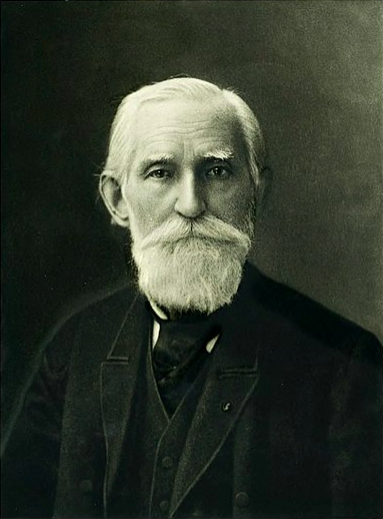
\includegraphics[width=9cm]{aggarwal_image1}
    \caption{Pafnuty Chebyshev (1821-1894) was a Russian Mathematician. He is widely acknowledged as the first person to think in terms of random variables. }
    \label{fig:1}
    \end{minipage}
\end{figure}


\newpage

\nnarticleheader{Foundations of Mathematics: Part II}{Dr. Mark Gottlieb, Haverford Faculty}
% hello from the past! remember to include this article in Issue V of the notebook. maybe add a little blurb before the next section about how this is a continuation of last year's article. best of luck! ~past Greer

\begin{center}
	\textit{The following article is Part II of Dr. Gottlieb's "Foundations of Mathematics"\\ 
	(inclding sections on \textbf{Formalism} and \textbf{Constructivism}).\\
	To read Part I (\textbf{Formalism} and \textbf{Constructivism})\\
	check out Issue IV of Newton's Notebook.}
\end{center}


\noindent
\textbf{Formalism}

    If mathematicians aren't studying unchanging objects or working out logical deductions, what are they doing?  We seem to be running out of possible ways of understanding what mathematics is all about.  In fact, there are other possibilities.  Some mathematicians, beginning about eighty years ago and inspired by the German mathematician David Hilbert, have argued that mathematics is really just a very complex game--the manipulation of symbols on paper according to rules.  The Transitive Property of Equality, mentioned above, is one example of this kind of rule, called a rule of inference.  Mathematicians who believe that mathematics is just a game with symbols are called \emph{formalists}.  Whereas Platonism and logicism never convinced the majority of mathematicians, for most of the twentieth century most mathematicians considered themselves formalists.  Both in the research papers they wrote and in the textbooks they authored, their approach was formalistic.  They communicated this way of thinking about mathematics to their students, and until recent decades, it dominated the advanced study of mathematics and mathematics education at other levels, as well.
     
     There are a number of peculiar consequences of the formalist view of mathematics.  One of the strangest is that formalists do not believe that mathematics is about numbers, spatial relationships, and patterns.  Instead, they will tell you that mathematics is really about 'marks on paper'.  Notice that they do not assign any meaning whatsoever to these marks--they might as well be gibberish.  As long as I follow the rules of inference correctly, according to formalists, I am a good mathematician.  When they are asked what numbers, triangles, and functions are, formalists reply, "Just names for symbols on a piece of paper."   Mathematical research, on the formalist view, is figuring out what new sets of symbols can be produced from the sets we already have using given rules of inference.\footnote{Interestingly, this seems to imply that computers could be quite good mathematical researchers, as they are essentially symbol-manipulating machines that follow formal rules.  A program that could check every mathematical statement for truth or falsity could do away completely with the need for human researchers in pure mathematics.}
     
      This explanation seems to conflict with the common experience we have when we are doing mathematics that we are thinking about numbers, shapes, and patterns, not just symbols.  For example, when we try to understand the properties of a number (like whether or not it is prime) or a shape, we often use our imagination to "turn things over in our mind".\footnote{The Dutch mathematician L.E.J. Brouwer was so impressed by this ability that he created an entire philosophy of mathematics called intuitionism.  Brouwer believed that all mathematical knowledge was based upon a direct intuition of the natural numbers.  Earlier versions of this theory can be found in the works of the great German philosopher, Immanuel Kant, and the mathematician Richard Dedekind.  Today few mathematicians accept Brouwer's approach, as it introduces a number of logical peculiarities.  For a brief survey, see Howard Eves, \textit{Foundations and Fundamental Principles of Mathematics}, pp.}  We think about breaking up the number in diferent ways, or we imagine the triangle in different positions.  From this mental process, we may discover new facts about numbers or triangles.  Mathematicians speak of "mathematical intuition" that enables them to make new discoveries or new conjectures.  This kind of intuition is a bit like having a hunch, a good understanding of a situation without spelling out all the details.  Sometimes we can just "see" that something is true without being able to say why.   Formalism essentially does away with the idea of mathematical intuition.  If mathematics is just moving symbols around, there doesn't seem to be any place for intuition about mathematical objects.  In fact, there isn't even a place for mathematical objects to begin with.
        
     When it comes right down to it, according to formalists, mathematics is really just making calculations.  Some of these calculations, or computations, as they are called in computer science, are simple, like multiplying 213 x 123.  Computations can, however, become very complicated, like figuring out whether or not a particular set of symbols follows by rules of inference from a set of basic symbols.
       
A program is a set of instructions that tells a computer to perform a list of operations in a specific order.  All programs have the same basic purpose: to turn input into output.  The computer receives input, it executes or carries out the program, then it displays an output.  For example, if my program tells the computer to multiply a number by 12, and my input is "7", the computer will display the output "84".  Mathematicians have developed a concept to express this relation of input to output, the well-known concept of a function. It is one of the most important of all mathematical ideas.  Here is the definition.
\begin{dfn}
A \emph{function} is a set of ordered pairs $(x,y)$ such that to each value of $x$ there corresponds one and only one value of $y$.  We often think of the value $x$ as being the input to the function, and $y$ as being the output.  (Note that $x$ and $y$ may or may not be numbers.)
\end{dfn}

We say, "$y$ is a function of $x$" if and only if the set of ordered pairs $(x,y)$ is a function and use the notation $ y=f(x) $ to indicate that $y$ is a function of $x$.  This means that $x$ is the input to the function and $y$ is the output.  We call the function $f$ and we can think of $f$ as being a rule that tells us how to compute the output $y$ from the input $x$. The set of all input values to a function is called the \emph{domain} of the function.  The set of all output values is called the \emph{range} of the function.

\begin{exm}{3}
The set $\{(1,2), (5,7), (7,\pi)\}$ is a function.  To each input there corresponds one only one output.  The domain is the set \{1,5,7\}, and the range is the set $\{2,7,\pi\}$.  If the first number in the ordered pairs is called $x$ and the second $y$, then we can write $y = f(x)$.
\end{exm}
\begin{exm}{4}
A function can be defined by an explicit rule.  Here is a simple case: $T(C) = 1.8C + 32$.  In this case we think of $C$ as being the input to the function and $T$ as being the output.  Some ordered pairs are ($0, 32)$, ($5, 41)$, and ($100, 212)$.  This function comes from the physical sciences.  Do you recognize it?
\end{exm}
\begin{exm}{5}
By plotting the ordered pairs deriving from a function we can generate the graph of a function.  In the above case we have:
\begin{center}
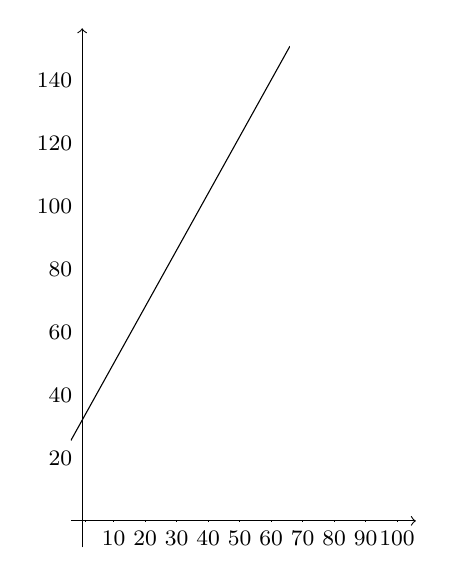
\begin{tikzpicture}[scale = 0.04][line cap=round,line join=round,>=triangle 45,x=1.0cm,y=1.0cm]
\draw[->,color=black] (-3.6,0) -- (105.97,0);
\foreach \x in {,10,20,30,40,50,60,70,80,90,100}
\draw[shift={(\x,0)},color=black] (0pt,2pt) -- (0pt,-2pt) node[below] {\footnotesize $\x$};
\draw[->,color=black] (0,-8.4) -- (0,156.45);
\foreach \y in {20,40,60,80,100,120,140}
\draw[shift={(0,\y)},color=black] (2pt,0pt) -- (-2pt,0pt) node[left] {\footnotesize $\y$};
\clip(-3.6,-8.4) rectangle (65.97,156.45);
\draw [domain=-3.6:65.97] plot(\x,{(--32--1.8*\x)/1});
\end{tikzpicture}
\end{center}
\end{exm}
\begin{exm}{6}
A function can be defined by a table of values, like the following:
\begin{center}
\begin{tabular}{|c|c|}
\hline 
$x$ & $y$ \\ 
\hline 
1 & 1 \\ 
\hline 
5 & 4 \\ 
\hline 
9 & 5 \\ 
\hline 
13 & 17 \\ 
\hline 
\end{tabular} 
\end{center}
Here, we can see that $y$ is a function of $x$, since to each $x$ corresponds one and only one $y$.  The domain is $\{1,5,9,13\}$ and the range is $\{1,4,5,17\}$.  A challenging problem is to come up with an explicit rule for the function.
\end{exm}
Armed with the idea of a function, we can better understand the formalist idea of mathematics and some of its limitations.  If mathematics is just rule-governed operations with symbols, then it looks as though it could be done by a computer without any help from a human being.  In fact, that's exactly what computers do; they perform operations on strings of symbols according to rules.  We input a string of symbols, press "Enter" and out comes another string of symbols.  In short, if formalists are right, mathematics could be done completely by machines, and human mathematicians would be unnecessary.

How would these machines work?  We would write a complicated program to figure out whether a particular string of symbols was a theorem.  Remember, a theorem is the conclusion of a formal proof, the last statement in a chain of logical steps. Our program, called a \emph{theorem-proving program}, would be able to check any string of symbols to determine whether or not it was a theorem. We could call this function T.  Its domain would be the set of all strings of symbols allowed in our symbol system, and its range would be 
\begin{center}
$\{\text{theorem},\text{not theorem}\}$
\end{center}   

For example, if the string of symbols  
\begin{center}
$\sigma\mu\kappa\upsilon\varsigma\Gamma$
\end{center} 
were a theorem in our system, we when we ran our program we would get
\begin{center}
$T(\sigma\mu\kappa\upsilon\varsigma\Gamma)= \text{theorem}$
\end{center} 
Once again, this means that the string '$\sigma\mu\kappa\upsilon\varsigma\Gamma$' can be derived from our basic assumptions by following the rules of inference.

The goal of the formalists was to show that all of mathematics can be represented by system of symbols and rules of inference.  All that was needed, they believed, was to find the right set of symbols and inference rules.  It is a remarkable fact that this goal turns out to be impossible.  In 1931 Kurt G\"{o}del (1906-1978), an Austrian logician, proved, using traditional mathematical methods, that, regardless of how we set up our system, there will always be certain strings of symbols that are neither theorems nor non-theorems in our system, but may recognized as true or false by mathematicians. 

In other words, our function $T$ simply won't work for those strings.  Mathematicians call G\"{o}del's result an \emph{Incompleteness Theorem}, because it shows that there is no way to create a formal system that can determine for any string of symbols it contains whether or not that string is a theorem.  There will always be strings of symbols that are `undecidable' in every formal system.  
G\"{o}del's work showed that mathematics cannot be completely turned over to machines, like computers, because there will always be some strings of symbols whose correctness can only be assessed by human beings.  There is no way to build a machine which we can be sure will be able to prove all true mathematical statements starting from a single set of assumptions.  To G\"{o}del, this result meant that mathematics must be something over and above any kind of symbolism.  This led him to become a Platonist, as we mentioned earlier.  G\"{o}del's basic idea was to show that all theorem-proving programs run into insurmountable problems when faced with statements like, "This statement is false."  This is similar to the difficulty we encountered in our discussion of Russell's Paradox.

\noindent
\textbf{Constructivism}

It looks as though none of the approaches we have so far considered gives an entirely adequate account of the nature of mathematics.  To summarize, we have seen that mathematics cannot be about things that are completely separate from the physical world; it is not purely logical, and it seems to be more than just a collection of symbols.  During the latter half of the twentieth century it became increasingly clear that none of the traditional ideas about mathematics were entirely correct.  Some mathematicians began to suggest that, perhaps, mathematics is a much more complex activity than anyone had imagined.  In fact, it began to look like each of the traditional ideas covered only part of mathematics. 
 
     A number of mathematicians and philosophers in recent years have suggested that to understand mathematics we will need to take its many different aspects into account.  Above all, these mathematicians suggest that mathematics is a human creation. Let us call this point of view \emph{social constructivism}.  Its chief proponents include the Hungarian mathematician Imre Lakatos, the British philosopher Karl Popper, and Paul Ernest, a British educational theorist.  According to these men, our mathematical knowledge does not rest on unshakeable foundations, like a direct awareness of numbers or shapes, as the Platonist and intuitionist  claim.  Neither does it rest upon logic or basic facts about sets.  Instead, constructivists believe that mathematics is a creative product of human activity.  They believe that numbers, geometrical shapes, and mathematical patterns were invented by human beings, originally for the purpose of solving practical problems.  For example, the Egyptians introduced the right triangle to assist them in agriculture and architecture; the Babylonians introduced numerals as aids to counting and record-keeping. 
      
     At first triangles and numerals were only tools, like hammers and saws.  Eventually, however, people began to raise questions about the relationships between the parts of a triangle or about whether or not a particular number was prime.  These questions have correct answers, and those answers do not depend upon anyone's opinion.  Human beings invented numbers, according to constructivists, but they did not invent the \emph{properties}, or basic facts about, numbers.  Once numbers have been invented, they come to have a life of their own, much like words, or laws, or Shakespeare's plays.  Constructivists speak of mathematical problems as "autonomous", meaning that they are not invented by us.  Once mathematical ideas have been invented, certain kinds of questions naturally arise.  These questions lead to investigation, to making educated guesses or conjectures, and to efforts to develop proofs.  Lakatos writes, 
\begin{quote}
          mathematics does not grow through a monotonous increase of the
          number of indubitably established theorems, but through the incessant
          improvement of guesses by speculation and criticism, by the logic of 
          proofs and refutations. \footnote{Qtd. in Hersh, \textit{What is Mathematics, Really?}, p. 211 }
\end{quote}  
          
Mathematical results are consequences of our invention of mathematics, but they are unintended consequences.  In other words, mathematics grows and changes in unpredictable ways as we work at it.  This, of course, is also true of other human activities; as Popper says, we often get more out than we put in. 
 
For example, as an artist works on a painting, the development of the painting affects how he does his work.  He might not realize that he was really painting a self-portrait when he thought she was painting a portrait of someone else.  She  doesn't realize this until she begins actually to put paint on the canvas and sees how things are turning out.  As another, more mathematical, example consider a complex game, like chess.  All the rules of chess are man-made, products of the human mind.  Nevertheless, as you may be aware, there are many principles or main ideas of chess strategy that were not completely understood until the game had been played for thousands of years.  These principles were not deliberately included in the rules; they were unintended consequences.  Einstein once remarked, "My pencil is cleverer than I am."  He meant by this that he often did not see the consequences of his ideas until he put them down on paper and began to work with them.  According to constructivists, the same is true of mathematics:  we do not fully understand mathematical ideas until we begin to work with them.  Thus, on a constructivist view, a proper mathematical education will not have its basis in mastering an established body of mathematical knowledge by rote but, rather, will emphasize the importance of the student's reconstructing the process of mathematical discovery underlying fundamental results.  In working results out for himself, the student is able to participate directly in the act of effectively employing mathematical tools and, perhaps--in extraordinary cases--advancing the development of mathematics itself, if only by criticizing standard assumptions.

The great strength of constructivism lies clearly in the emphasis it places upon the informal, creative, and evolving nature of mathematical thought, aspects that are all but neglected by the approaches considered earlier.  To be sure, constructivists have been quite right to emphasize the informal, creative, and evolutionary nature of mathematical thought.  It is undoubtedly true that classical approaches to mathematical thinking have almost universally been guilty of treating mathematical ideas as though they arrived ready-made in the human mind, whereas it has only been by a lengthy process of trial and error, of conjecture and refutation, that mathematics has reached its present form.  But there is a great difference between describing the process of mathematical discovery and describing the body of knowledge discovered.  If mathematical knowledge is, as constructivists maintain, a product of human convention, it is clearly a most extraordinary product.  It is true that certain social conventions, like language, customs of dress, or even traffic laws may come, in time, to seem to be both universal and necessary, but as American drivers may recognize when traveling in Britain, or French speakers in Germany, these conventions are quite easily given up when the circumstances require it.  

This is not true, however, of mathematical judgements, which seem to hold in all places and times and to admit of no possible alternatives.  It seems to be both certain and necessary that, for example, $7 + 5 = 12$.  There seems to be no question of giving up
our belief in this statement.  It is simply inconceivable, short of confusion, that we should believe that $7 + 5 = 13$.  This inconceivability accounts, in large part, for
the apparent necessity of mathematical truths.
  
Constructivists, as we have seen, are well aware of the special status of mathematical knowledge, and, as indicated above, have generally explained the apparent objectivity and universality of mathematics by holding that the relationships among mathematical ideas are not man-made, although the ideas themselves are.  But this view really is not very different from that of the logicists, namely, the view that mathematics consists of nothing more than drawing logical conclusions from given assumptions.  The assumptions may be man-made ideas, but the process of discovering relations between them is not distinguishable from logic, and we saw earlier that logic does not completely capture the nature of mathematical activity.  Constructivism contains important insights, but it fails as a complete framework for understanding the nature of mathematics. 

\noindent
\textbf{Conclusion: One Discipline, Many Faces}

 During the latter years of his life, the philosopher Ludwig Wittgenstein, one of the most influential thinkers of the twentieth century, became well known for his opposition to the notion that it is, or ought to be, possible to state precise definitions of terms employed in our ordinary experience.  Thus, speaking of the term "game", for example, we might attempt the following definition: "a competive activity aiming at a goal".  But solitaire is a game, and it is not competitive.  Moreover, frisbee is a game, but its "goal" is far from obvious.  In this way, our efforts at definition may come to nought.  Nevertheless, games do indeed share what Wittgenstein called a 'family resemblance' by which we are able to recognize them.  This resemblance may not be easily articulated, and there may well be cases which seem to lie at the periphery (Is surfing a game?), but most competent users of our language would agree about what constitutes a game and what does not (Performing brain surgery is \textbf{not} a game.)  There are good reasons for supposing that mathematics has much the same nature.
 
     We have seen that the most strenuous efforts of mathematicians to define their subject in straightforward terms have not been successful, or, more, correctly, have only been partially successful.  In the last analysis it seems fair to say that each of the principal approaches to the foundations of mathematics has identified one aspect of mathematical thought and constructed an account that places a more or less exclusive emphasis on that aspect.  For example, Platonism derives its plausibility from emphasizing the apparent objectivity, universality, and necessity of mathematical knowledge.  On the other hand, logicism is rooted in the observation that mathematics is the most logically rigorous branch of human knowledge, exhibiting the highest possible degree of structure, coherence, and rationality.  It is this deductive structure that makes mathematics universally applicable to other fields and enables mathematical thinking to be employed in all walks of life.  Mathematics is unique among disciplines in its use of precisely defined terms and symbols.  In no other field of human activity is symbolism employed in such a manner. This, no doubt, accounts for the appeal of formalism to a generation of eminent mathematicians.  Finally, mathematics has much in common with both art and science.  With the arts, mathematics shares a deep sense of aesthetic value; nearly all mathematicians would agree that their subject is beautiful.  Furthermore, like the arts, mathematics is a creative discipline, with new ideas and methods constantly being developed.  Like the sciences, mathematics is in pursuit of truth, and any mathematical conjecture is subject to criticism and revision, much like  a scientific theory.  Like great theoretical ideas in the sciences, mathematical ideas that unify seemingly disparate branches of the discipline represent the supreme intellectual achievement of the mathematician.
     
It seems then, that mathematics has not yet been defined adequately.  Perhaps the search for such a definition is fundamentally misguided, or perhaps an ingenious mind may someday adequately express the nature of mathematics.  Whatever may be the case,  several aspects of mathematics will be  especially important to its growth and development in the 21st century.  Let us discuss each of these in turn.
     
First, although its applications will increase exponentially in the future, mathematics will continue to be an inherently abstract discipline, and its level of abstraction will continue to rise.  The abstract nature of mathematics, though often an obstacle to the layperson, is precisely what gives mathematics its universal power to act as a model for nearly every aspect of reality, from the large-scale structure of space-time to the complex workings of nervous systems to the behavior of the nuclei of atoms.   It is nothing short of amazing that on many occasions discoveries of mathematicians working at problems belonging to "pure" mathematics have become cornerstones of scientific theories and technological advances of the widest significance.  This process began in the seventeenth century with Newton's and Leibniz's work on integral calculus and reached a pinnacle in the application of the abstract geometry of Riemann to Einstein's General Theory of Relativity.  Spectacular examples in recent times include the development of the modern computer from the theoretical ideas of Alan Turing, a British mathematician, as well as the ingenious use of binary numbers to make possible the Information Age.
      
Second,  mathematics will continue to grow, generating new methods, concepts and problems.  Its growth will be twofold.  On the one hand, it will be driven by imperatives deriving exclusively from mathematics itself and the many unsolved problems that continue to attract the best mathematical minds.  While solutions are are clearly desirable, as a by-product of ongoing reseach new questions are almost certain to arise and generate yet more unsolved problems.  In this way, the field of mathematical inquiry enlarges and deepens in scope.
       
Mathematical work will also be stimulated by the drive to master the complexities of both the natural and the human world.  This imperative will come not only, as it has traditionally, from physics, but also, and increasingly, from molecular biology, medicine, economics, and neuroscience.  The advent of ever-greater computing power will make it possible to model in real time (or hyper-real time) such phenomena as information processing in the visual cortex, the pharmacological effects on the body of new medicines, and the behavior of large-scale social and economic systems.  At the outer limit we can imagine mathematical models so powerful they can emulate the human mind, both in its cognitive and affective aspects.  We are pursuing that goal today, and the prospects are good that we will attain it, provided we have the insight and ingenuity.

     In the coming century mathematical thought will be, more than ever before, intimately linked to its embodiment in technology.  To be sure, mathematics has always been a calculational science. Geometry takes its name from surveying the earth, while trigonometry has similar origins; in modern times we have the logarithms of Napier, the calculus of Newton, and Charles Babbage's Analytical Engine.  Every generation of mathematicians has made improvements upon the technological capabilities of its forebears.  But in the present situation things are different.  Today, owing to the integration of advanced technology into the framework of everyday life, mathematicians encounter a world already laden with mathematics.  The digital cameras, tablet computers, smartphones, and wifi networks found everywhere in the developed world are a living embodiment of the collective mathematical genius of many generations.  In mathematics today, the primary tool of creative work (the computer), the vehicle of communication (the Internet), and the principal product (the algorithm or computation) are inherently bound up with a technologically complex world.  Paper and pencil will not disappear from the mathematician's desk, nor will his desire to construct proofs that can meet the highest standards of rigor, but one may safely assume that mathematicians will devote the lion's share of their time and energy in the coming century to making the fullest possible use of technology both to develop mathematics on its own terms and to bring mathematics to bear on real-world problems.
       
Certainly, there is no shortage of problems.  Future generations must develop new sources of energy.  They must work to restore the earth's ecological balance.  Medical researchers must make progress in the fight against AIDS, cancer, and heart disease.  Economists must develop reliable models of economic growth that are both sustainable and supportive of basic human needs.  Educators must develop methods of effective teaching so that every student will be able to participate in a complex global economy.  In the coming century the world leaders will face the dual challenge of empowering the creative energies of humanity while at the same time taking adequate precautions, so that individuals bent on violence cannot convert their ill will into acts of mass destruction merely by pressing a button.
  
These tasks will require great imagination.  They will demand attention to detail and rigorous analysis.  They will depend upon technological innovation.  In short, they are tasks ideally suited to the mathematician of the twenty-first century.  


\newpage

% Begin the applied math section
\nnwallpaper{2021_Applied_Math_Page_Border.pdf}
\def\currentTitleWallpaper{2021_Applied_Math_Title_Page_Border.pdf}

\addcontentsline{toc}{part}{Applied Mathematics}
\nnimagepage{2021_Applied_Math_Section_Title.pdf}

\nnarticleheader{Oligopoly and Game Theory}{Mitav Nayak, Haverford '22}

\noindent
\textbf{Introduction}

\textbf{Game theory}, sometimes dubbed the “science of strategy,” allows exports to mathematically analyze the human decision-making process. The modern version of the field was initiated in the mid-twentieth century by the Hungarian-American mathematician John von Neumann, who released a proof regarding two-person zero-sum games. Shortly after, Oskar Morganstern, a German-Austrian economist, collaborated with von Neumann to publish \emph{Theory of Games and Economic Behavior} in 1944. Many suggest that this book in a sense founded modern game theory. In the following years, game theorists would discuss the topic’s broad range of applications in fields such as computer science, applied mathematics, politics, and economics. This article will discuss a particular application of game theory in economics: oligopoly.

\noindent
\textbf{Oligopoly}

Most likely, many have heard of the term monopoly, which occurs when there is only one firm in a market that supplies a good or service. However, a far more common occurrence in an economy is an oligopoly. In this case, rather than just one firm, a small group of firms controls the supply of a good or service. Cell phone providers, airlines, mass media, and big tech firms are just a few examples of oligopolies in our economy today. According to Statista [1], just four firms control about 65\% of the airline market today.

\begin{figure}[htp]
    \centering
    \begin{minipage}{9cm}
    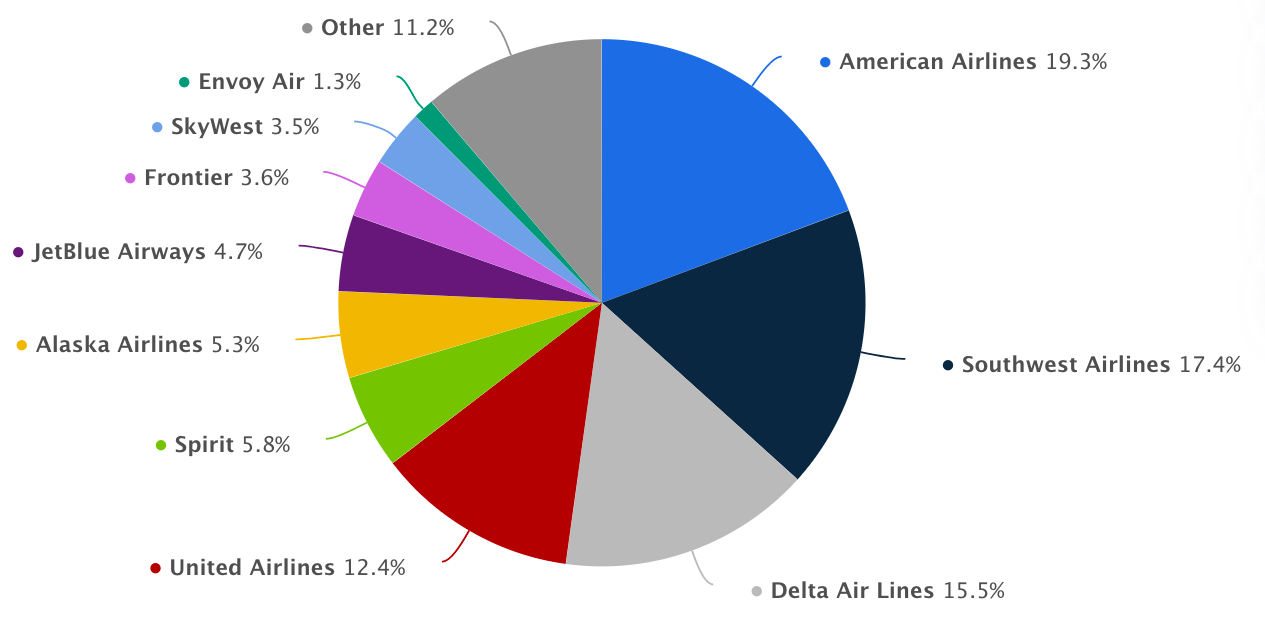
\includegraphics[width=9cm]{nayak_image1}
    \caption{American Airlines, Southwest Airlines, Delta Air Lines, and United Airlines may have an \textbf{oligopoly} on the market for air travel.}
    \label{fig:1}
    \end{minipage}
\end{figure}

	When studying most markets, economists assume that there exists \textbf{perfect competition}, where all products are the exact same, and buyers and sellers are so numerous that no single buyer or seller can influence the price. In these markets, firms are price takers, meaning that they must accept the market price, which is determined by supply and demand. On the other hand, oligopoly is an example of \textbf{market power}, which is a type of market failure that occurs when one or more firms can influence the price of a product. Since there is little competition, firms may be price makers, meaning they can artificially raise prices and consumers will still buy the product. Unlike with a monopoly, where the firm has no competition, firms in oligopolistic markets still have competitors, so their ability to raise prices is more limited. For example, if American Airlines were to raise their price drastically, travelers would simply switch to a different airline.

	Firms may use non-price competition to compete with other firms in an oligopolistic market, with methods like advertisement, branding, or location. In a perfectly competitive market, firms would likely not rely as much on non-price competition because every product would be the same. Granted, a perfectly competitive market is almost always an oversimplification, but there are markets where the products are extremely similar—for example, the market for salt. In a monopolistic market, the firm will not use methods of non-price competition because it has no competitors. Therefore, non-price competition is most common in oligopolistic markets, where the products are different, and there are a few firms competing with each other. To understand the firms’ decisions and interactions as they engage in this competition, we can call upon the science of strategy.


\noindent
\textbf{Game Theory}

\noindent
\emph{The Prisoners' Dilemma}

The most standard example of game theory is the prisoners’ dilemma, a situation in which two criminals are caught and taken into police custody. Here, we will call them Prisoner A and Prisoner B. In our example, the police have evidence that both individuals have committed a crime, say petty theft, that will put them in prison for 1 year. However, the police believe that both criminals have committed a worse crime, such as a major bank robbery. The prisoners are separated, so they cannot communicate, and they are given the following information:

\begin{itemize}
  \item If both confess to the bank robbery, both will serve 5 years in prison.
  \item If both refuse to confess, both will serve six months in prison for the lesser crime (petty theft).
  \item If one remains silent and the other confesses, the one who confesses will be set free, and the other will serve 10 years in prison.
\end{itemize}

We can see the dilemma in a matrix:

\begin{figure}[htp]
    \centering
    \begin{minipage}{9cm}
    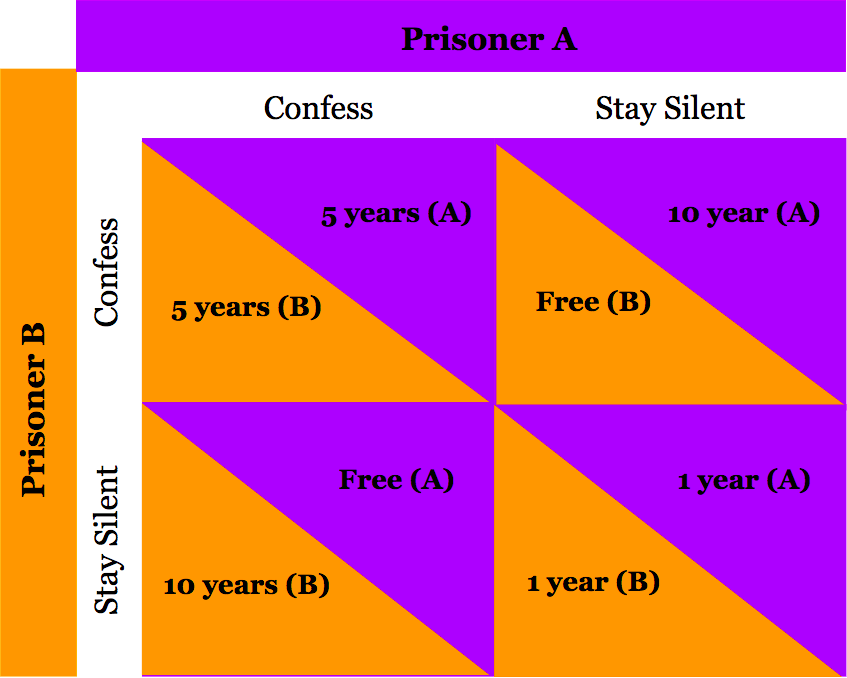
\includegraphics[width=9cm]{nayak_image2}
    \caption{The Prisoners’ Dilemma.}
    \label{fig:2}
    \end{minipage}
\end{figure}

    \pagebreak
    Since both prisoners are held separately and cannot communicate, they will act to maximize their own self-benefit. We can look at the situation from Prisoner A’s point of view. If Prisoner B confesses, Prisoner A’s best decision would be to confess and spend 5 years in jail instead of 10. If Prisoner B stays silent, Prisoner A should still confess so he can spend no time in jail instead of 1 year. Prisoner B will look at the situation in the exact same way. In this example of the prisoners’ dilemma, both prisoners have a \textbf{dominant strategy}, which is—in game theory—a strategy that is optimal no matter how other players act. Because both prisoners should confess regardless of the other prisoner’s decision, this is their dominant strategy. Acting in self-interest and unaware of the other individual’s decision, rational prisoners will confess even though they could have both remained silent to minimize their total prison time.

\noindent
\emph{Nash Equilibrium}

The case we have just examined demonstrates the \textbf{Nash Equilibrium}, where all players do not change their strategy, given the strategies of the other players. It is named after John Nash, an American mathematician whose thesis containing the equilibrium won him the Nobel Prize in Economic Sciences.

\begin{figure}[htp]
    \centering
    \begin{minipage}{9cm}
    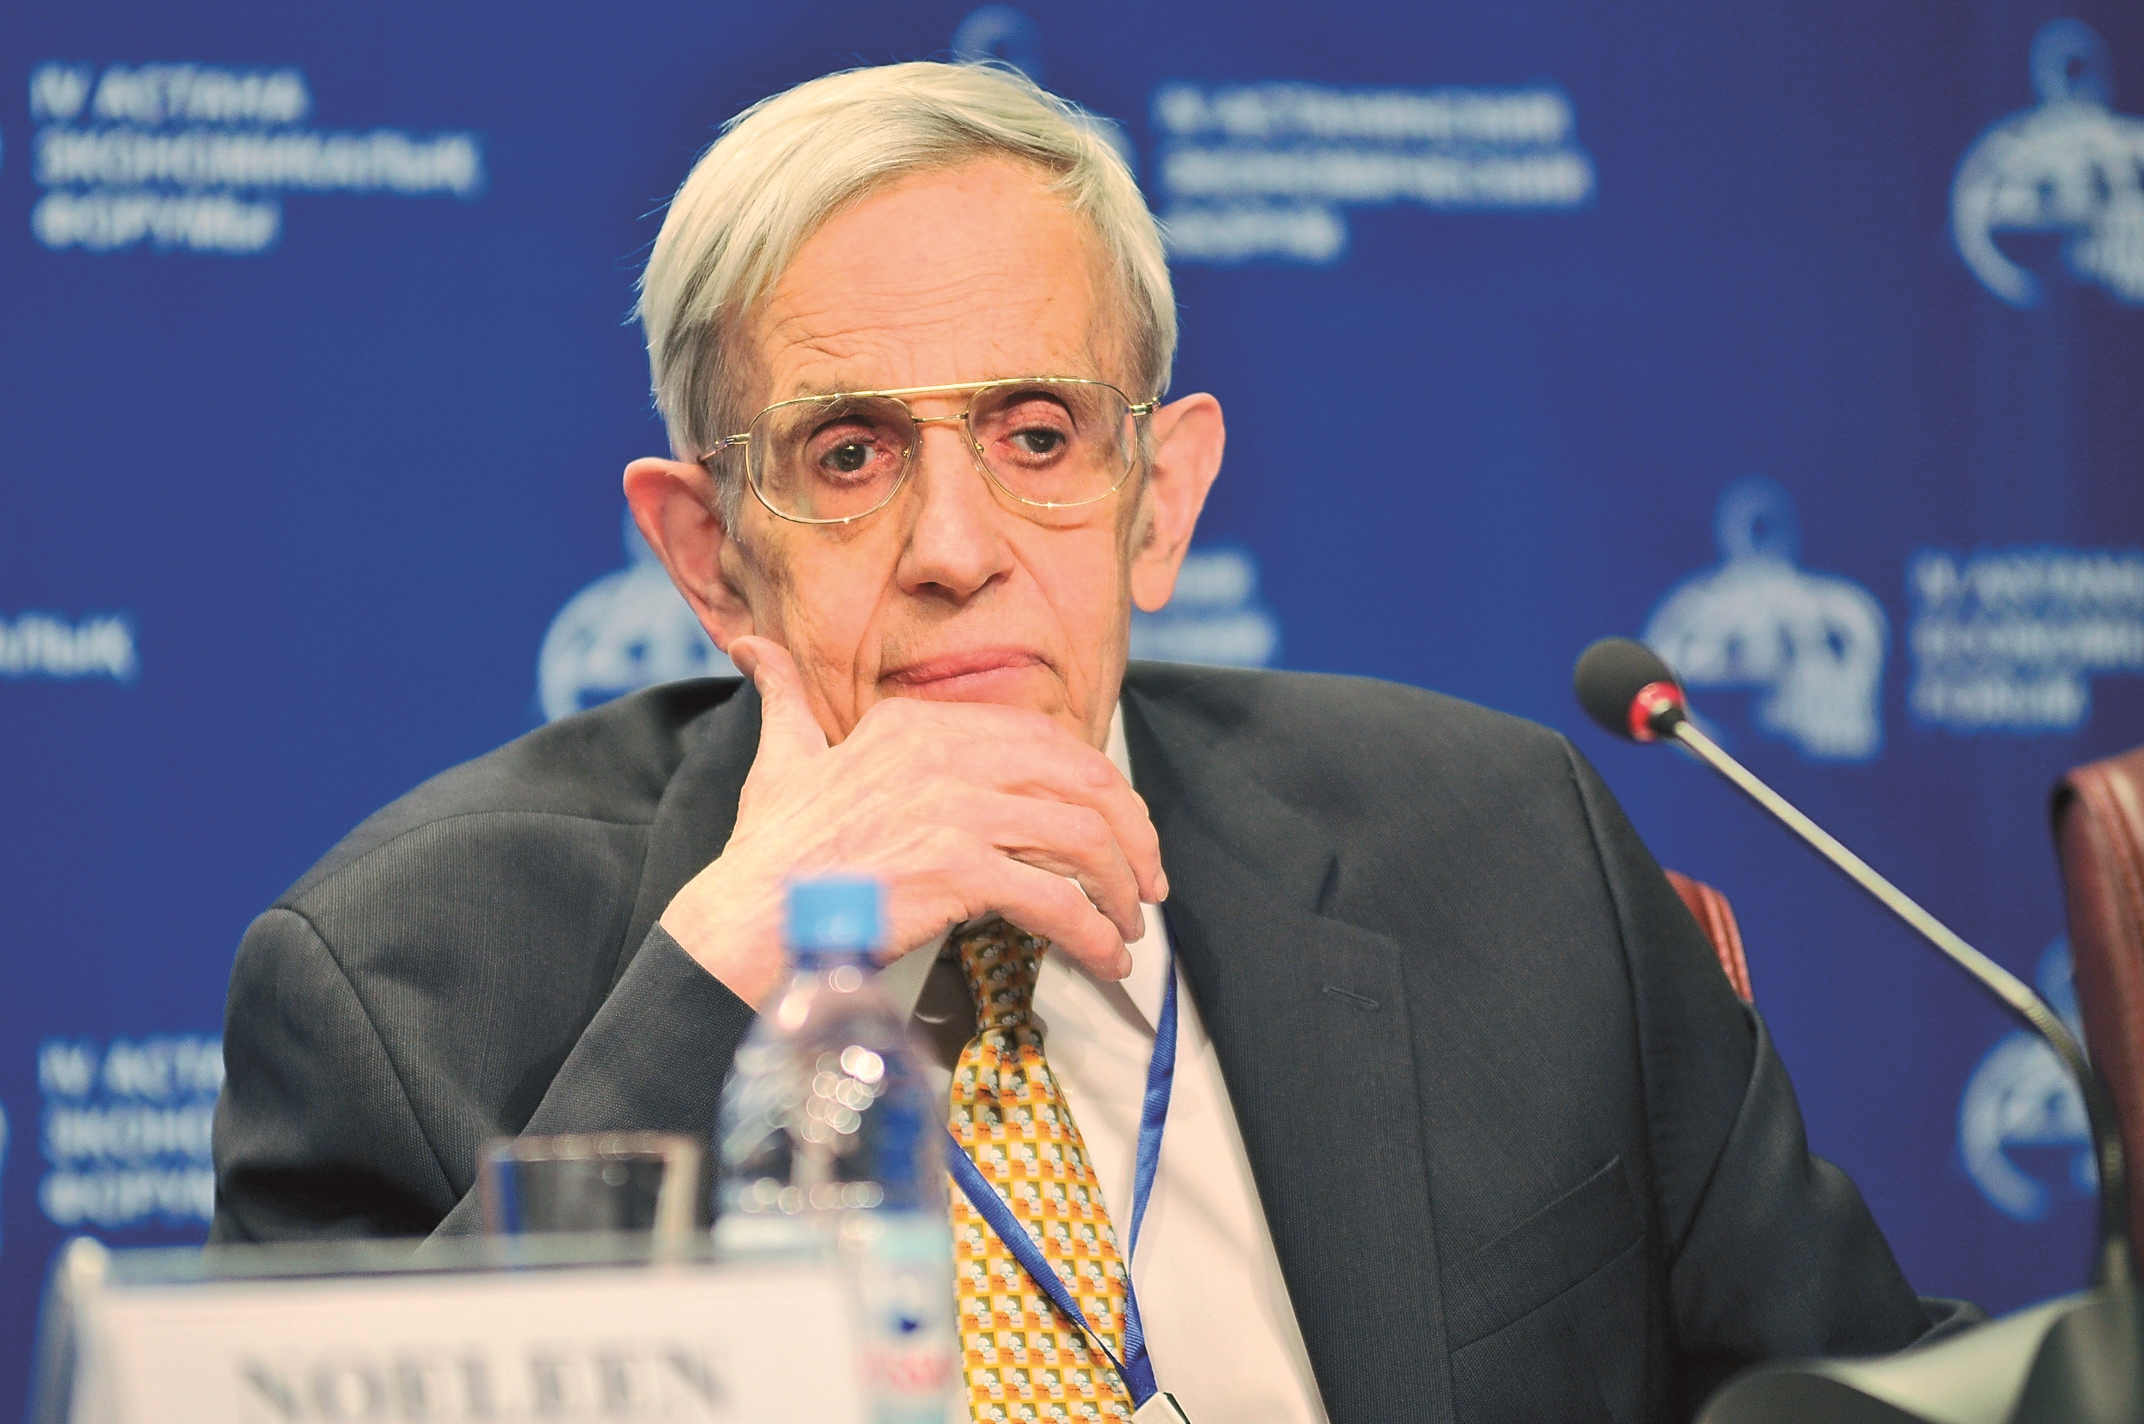
\includegraphics[width=9cm]{nayak_image3}
    \caption{John Nash in 2011 [2]}
    \label{fig:2}
    \end{minipage}
\end{figure}

\pagebreak
In the years following the publication of Nash’s thesis in 1950, economists examining oligopoly have relied heavily on the ideas Nash outlined. We have seen how the equilibrium is present when studying prisoners’ decisions, and we can now extend these ideas to firms.


\noindent
\textbf{Oligopoly and Game Theory}

\noindent
\emph{Advertisement}

Let us consider a \textbf{duopoly}, an oligopoly where two firms control supply. These two firms—say Coke and Pepsi—dominate the market for soft drinks and engage in non-price competition in the form of advertisement. We can construct a \textbf{payoff matrix}, as we did with the prisoners’ dilemma, to examine possible outcomes in this hypothetical situation:

\begin{figure}[htp]
    \centering
    \begin{minipage}{9cm}
    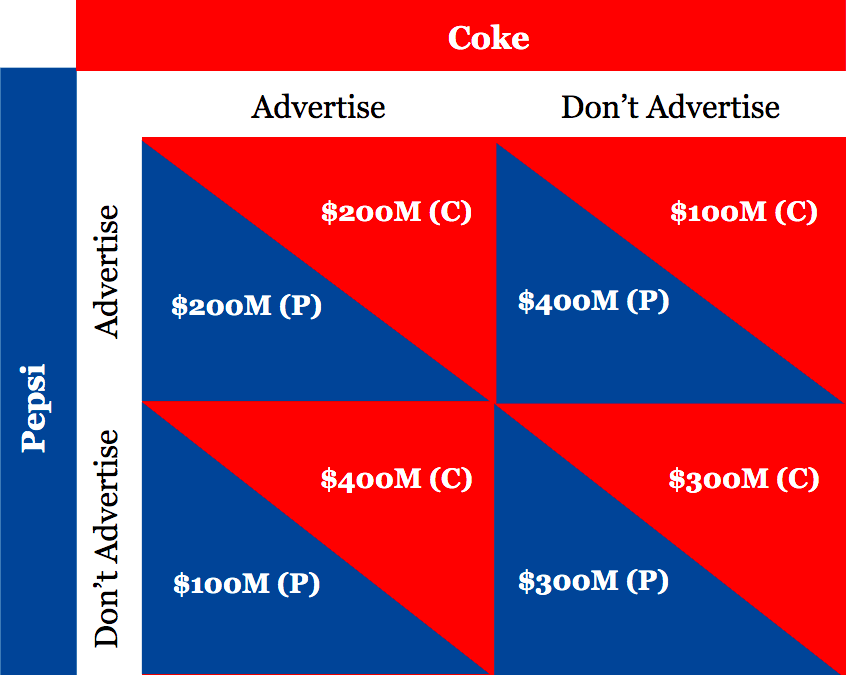
\includegraphics[width=9cm]{nayak_image4}
    \caption{A payoff matrix for Coke and Pepsi depending on their decision regarding advertisements.}
    \label{fig:2}
    \end{minipage}
\end{figure}

\pagebreak
As we can see in the matrix, the situation is very similar to the prisoners’ dilemma. If Pepsi does not advertise, Coke’s best strategy is to advertise, so they can gain \$400 million in profits instead of \$300 million. If Pepsi does advertise, Coke’s best strategy is to advertise, so they can gain \$200 million instead of \$100 million. Regardless of what Pepsi chooses to do, Coke should advertise: this is their dominant strategy. The situation from Pepsi’s point of view is exactly the same. This will lead to both firms advertising and gaining \$200 million in profits; this is a Nash equilibrium, since no firm will have an incentive to change their strategy, given what the other firm is doing.

Still, we can see that both Coke and Pepsi could have been better off if they had both chosen not to advertise (maybe they would have saved on the costs of creating and purchasing advertisements). We saw in the prisoners’ dilemma that the prisoners were isolated and could not speak to one another, so they could not devise a strategy together. But in this situation, could Coke and Pepsi discuss the situation with each other and increase both firms’ profits by not advertising? The answer is no: this would be \textbf{collusion}.

If firms in oligopoly were allowed to conspire with one another, forming what is called a \textbf{cartel}, they would simply band together and raise all of their prices collectively. For example, if Coke and Pepsi were the only two soft drinks, and both doubled their prices, consumers would have nowhere else to purchase soft drinks, so the firms would both increase their profits. However, this would be inefficient, since prices have been raised artificially, and it would also be unfair for consumers. To prevent situations like these from occurring, Congress has passed \textbf{antitrust laws}. Since they were first introduced in the United States in the late 1800s, these laws have encouraged competition and free markets. Still, they have not completely prevented firms from colluding, and even in the 21st century, there have been a handful of antitrust lawsuits.

\noindent
\textbf{Conclusion}

This article provided a brief overview of oligopoly and game theory. We investigated real-world examples of oligopolies and discussed market power. We introduced game theory and examined the classic example of the prisoners’ dilemma to illustrate the ideas of dominant strategy and a Nash equilibrium. Further, we constructed payoff matrices, discussed duopoly and market power, and we defined collusion, cartels, and antitrust laws.

The field of game theory and its applications in oligopoly are extensive. The science of strategy is a broad and far-reaching field, and as economists and game theorists continue to analyze behavior and markets, the applications will only continue to expand.



\pagebreak
\begin{thebibliography}{3}

\bibitem{} 
https://www.statista.com/statistics/250577/domestic-market-share-of-leading-us-airlines/

\bibitem{}
https://commons.wikimedia.org/wiki/File:John\_Forbes\_Nash,\_Jr..jpg

\bibitem{}
Mankiw, N. Gregory. Principles of Microeconomics. 8th ed., CENGAGE Learning Custom Publishing, 2016.

\end{thebibliography}


\newpage

\nnarticleheader{Fishing Reels Investigation}{Colin Kelly, Kiran Mistry, and Roch Parayre, Haverford '23}

\emph{"Fish on!"} is a common phrase used by many fishers to declare when a fish is hooked on the line and they begin to reel it in. Of course, this phrase means that there is a “fish on” the line. With this in mind, think about the phrase \emph{“Moon on!”} It seems silly, right? How could it even be possible to reel in the moon with a fishing rod? Even if it were possible, wouldn’t it take millions of years? Well, in this investigation, our group dove into this hypothetical situation and tried to answer the question of how long it would take to reel in the moon with a constant reeling speed, using four different kinds of fishing rods.

To answer this question, we needed to look at the idea of rotary motion and analyze how it applies to a fishing rod. The first thing we decided was that we should have a constant reeling speed — that is, constant speed of hand motion. Four handle revolutions per second seemed like a realistic pace that was fast but a human could definitely hold. Because we decided that the handle turn speed would be constant, that meant that the angular velocity of the reel would be constant too. However, we discovered that even though the angular velocity would be constant, the linear velocity of the outside of the reel, which defines the speed that the fishing line is reeled in, would not be constant. This is because as string wraps around the reel, it adds to its circumference. This seemingly simple and small detail was actually the hardest part of cracking this problem. We learned through investigating that the effects of this slow increase in the circumference of the reel are much more complicated than they seem on the surface. This
discovery also made us immediately realize that there would definitely be upwards curvature in the graph of this equation because the rate of change, or slope, increases over time.

Before beginning our work, we also had to structure and define some of the details of the problem we were trying to solve. The first one was that the length of the entire string would be exactly the distance from earth to the moon. This means that when you start to reel in the fishing line, the reel is bare. So, during the reel’s first revolution it has no string on it. Another thing that we decided was to make the width of the reel the same as the width of the string. This means that as revolutions are completed, the fishing line immediately begins wrapping on top of itself, not next to the previously wrapped string. After everything was agreed upon, we began to explore our problem and how to solve it.

Our first step was to determine the different types of fishing rods that we would use for the investigation. Through our research, we found three distinct types: baitcasting, spinning, and spin cast. Baitcasting rods are most often used with heavier lures and ones that can be handled with more force. Baitcasters are better for precision, but they require more experience. Spinning reels, which are by far the most popular type, are much more simple and designed for the use of lighter baits. Spin cast reels are the most basic and cheap, and are primarily made for beginners. After learning about the different types of fishing rods, we began research on the more specific aspects of fishing rods. The reel is the part that actually pulls in the fishing line, and it is where the string wraps around as it gets pulled in. The handle is turned by the person operating the fishing rod, and spins the reel at a speed determined by the gear ratio between them. The gear ratio tells you how many times the reel turns per every revolution of the handle. After developing a solid general understanding of how fishing rods work and the variations between different models, we selected four fishing rods that we would use in our investigation. For each rod, wefound the gear ratios and the amount of string reeled in by each handle turn in inches. Then, with these two pieces of information, we calculated the base circumference of each fishing rods’ reel. This could easily be done by dividing the amount of inches reeled in per handle turn by the gear ratio between the handle and the reel.

$$\frac{\text{number of inches}}{\text{1 handle rev}} \times \frac{\text{1 handle rev}}{\text{number of reel rev}} = \frac{\text{number of inches}}{\text{reel rev}}
$$

The product of these two proportions is the number of inches of string reeled in on the first reel revolution, or the circumference of the reel.

At this point, there were only a few other values that were left to determine. Because we decided that our constant handle speed would be four handle rotations per second, multiplying this value by the gear ratio gave us the number of rotations of the reel per second. Then, all that was left was to determine how thick the fishing line was for each fishing rod. The thickness of the line has an astounding impact on the results of this problem, as it determines how quickly the rate that string is reeled in grows. This table displays all the necessary values for each rod:




\begin{center}
\begin{tabular}{|l|l|l|l|l|l|}
\hline
Type of Rod                                                                       & \begin{tabular}[c]{@{}l@{}}Gear \\ ratio\\ (reel:\\ handle)\end{tabular} & \begin{tabular}[c]{@{}l@{}}Line reeled\\ in per \\ handle\\ revolution\\ (in)\end{tabular} & \begin{tabular}[c]{@{}l@{}}Number of \\ reel rotations\\ per second\\ (rev/sec)\end{tabular} & \begin{tabular}[c]{@{}l@{}}Circum-\\ ference\\ of reels \\ (in)\end{tabular} & \begin{tabular}[c]{@{}l@{}}Width of\\ fishing\\ line (in)\end{tabular} \\ \hline
\begin{tabular}[c]{@{}l@{}}TATULA\\ TYPE-R\end{tabular}                           & 8:1:1                                                                    & 33.9                                                                                       & 32.4                                                                                         & 4.185                                                                        & .009                                                                   \\ \hline
\begin{tabular}[c]{@{}l@{}}REV04\\ SX-HS\end{tabular}                             & 7:3:1                                                                    & 30                                                                                         & 29.2                                                                                         & 4.110                                                                        & .009                                                                   \\ \hline
\begin{tabular}[c]{@{}l@{}}Lew's\\ American\\ Hero Speed\\ Spin Reel\end{tabular} & 6:2:1                                                                    & 32                                                                                         & 24.8                                                                                         & 5.161                                                                        & .018                                                                   \\ \hline
\begin{tabular}[c]{@{}l@{}}Zebco \\ Bullet\\ Spincast \\ Reel\end{tabular}        & 5:1:1                                                                    & 29.6                                                                                       & 20.4                                                                                         & 5.803                                                                        & .0148                                                                  \\ \hline
\end{tabular}
\end{center}




To make things easier when writing equations, we decided to use the TATULA TYPE-R fishing rod for all of our primary calculations. The table above made it easy to change the values in our equations after they were written.

As we investigated how best to calculate how long it would take to reel in the moon, we realized that this would depend mostly on the changing circumference of the reel. The circumference of the reel is how much line is reeled in on a certain rotation. However, this circumference is not constant. As more and more fishing line is reeled in, it adds to the radius (and therefore circumference because the equation for circumference is $c=2\pi r$) because the string is wrapping around the reel as it spins. However, what makes this problem both interesting and difficult is the radius is not always increasing. The radius only increases once a full rotation is completed because that’s when a new ‘layer’ of fishing line begins overlapping with previous ones. This pattern of only increasing after a certain interval reminded us of a step function. The specific step function that it required, we soon discovered, is a floor function, one that rounds the input down to the nearest integer. It’s a floor function because in a half revolution of the reel, the radius is still what it was at the completion of the previous full revolution. Because of this, the function would have to round down instead of up.

At first, we started working on the equation in terms of circumference, because that was what we were trying to measure. But, we discovered that it would actually be easier to write the equation in terms of radius and then multiply the whole equation by $2\pi$. Because we were using the TATULA TYPE-R rod for our initial calculations, the radius of the bare reel was $113/(54\pi)$, the thickness of the string was $0.009$, and the number of reel revolutions per second was $32.4$. Using these three values, we determined the circumference of the reel in inches as a function of time in seconds to be: $C(x)=2\pi (0.009(\text{Floor}(32.4x))+113/(54\pi))$.

Once we had this function, we began our work to formulate a final function — one that modeled inches pulled in by the fishing rod as a function of time in seconds. If we found this equation, we could use it to solve for the amount of time it would take to reel in the moon by setting the output value equal to the distance from earth to the moon. However, we had no idea where to start.

After a particularly draining call one night, the members of our group went to sleep with a lot to think about. The next morning, two members of our group, Colin and Kiran, each had their own ideas of what the final equation would look like. The third member, Roch, was not adamant about either. Colin was certain that the function for circumference would somehow be related to the slope of the graph for the final equation. He tried many different methods that incorporated this idea by multiplying x by the entire circumference equation. But the biggest problem that this way of thinking faced was that there were many skips and jumps in the function that didn’t accurately model the amount of string reeled at any given time — a problem that came with using a step function. He tried fixing this by subtracting the amount of space that was skipped as a function of x from the equation, however because the jumps kept getting bigger, he could never find the right expression to model that space accurately enough.

Kiran’s idea, one that was very different from Colin’s, had to do with the second derivative of calculus. Taking the second derivative of something simply means to take the derivative twice. For a function, this means finding the rate of change of a rate of change, or the slope of a slope. Using this strategy, Kiran calculated the continuous rate of change of the radius of the reel for the first fishing rod — 2.916 inches every 10 seconds. Then, we changed the equation to model the rate of change for the circumference by multiplying the whole equation by $2\pi$. The equation he came up with for the first fishing rod was:

$$f(x)=(32.4\cdot x \cdot \frac{33.9}{8.1}) + (.018\pi)(x-1)
$$

However, checking it by hand revealed that this was in fact incorrect. It did not work because this equation was incapable of adding the fishing line added by previous rotations into the sum of the output. So, another equation had to be found.

Although both equation models were incorrect, they were part of the long process to determine what the correct equation really was. Kiran’s equation in particular inspired an idea. Because the only problem with the equation was that it could not add all of the previous string wraps and incorporate it into the y-value, all we had to do was alter the equation slightly to include these previous wraps. However, exactly how one could do that stumped us for a while.

Finally, after testing countless different methods that all failed, we found a certain Greek letter that we could possibly use. It was Sigma, or $\Sigma$. In mathematics, Sigma represents the summation function. The summation function is unique because it can add all of the integers in an arithmetic sequence. The lower space is for the lower bound, and the upper space is for the upper bound. The space on the right is for the function that all of the integers will be inputted into. Then, Sigma takes the sum of all the outputs of the function on the right when each integer 10 in the defined set is inputted. For example, the value of $\sum_{n=1}^{10} n$ is 55. The lowest integer is 1 and the highest integer is 10, so Sigma takes this: $1+2+3+4+5+6+7+8+9+10=55$. You can also put a function into the space on the right of Sigma. So, $\sum_{n=3}^{5} 2n+1 =2(3)+1+2(4)+1+2(5)+1 = 27.$

After playing around with the summation function, we discovered that it solved our biggest problem in finding the correct equation. It was capable of adding up a large number of distinct values in a very clean way that we could control. All that was left to do was to figure out how to integrate Sigma into an equation that gave us the most accurate solutions.

The hardest problem to solve with integrating Sigma into an equation was where the input value for the equation $(x)$ should go. We quickly dismissed the possibility that it should go in the lower bound. The point at which string begins getting added to the reel does not change; it is fixed. But between the other two options, we could not decide. It called for some more in-depth research of Sigma. We tried looking through websites for explanations of what each part of the function meant and what changing them would do, but for some reason there really is not much information out there on the summation function. So, we resorted to trial and error on Desmos to see what changes to Sigma would affect which parts of the graph. However, unfortunately Desmos really struggles with the summation function. It takes a very long time to load changes and show them in the graph, so that really slowed us down. But eventually, we were able to form a semi-solid understanding of Sigma. In our case, the function on the right of Sigma would include the thickness of the string, because that is what is being added each rotation. And because the thickness of the string is constant, $x$ definitely cannot be included there. But, $x$ fits perfectly into the upper bound of the Sigma function. This is because the number of rotations defines how many layers of string is being added. So, the upper bound of the Sigma equation is the number of rotations, or $x$ times the number of reel rotations per second. By plugging in the specific values for the TATULA TYPE-R rod, we got this equation:

$$f(x) = \frac{(32.4x)33.9}{8.1} + (\sum_{n=1}^{32.4x} (.018\pi)(n-1))
$$

We put this equation into Desmos, and after waiting for it to load, we tested some points that we knew had to be on the graph after finding them by hand. Lo and behold, the equation worked. After talking it over, we agreed that this was the correct equation.

After finding the equation for the TATULA TYPE-R rod, we used it to formulate the other 3 equations by replacing the numbers so that they are those of the proper rod. This saved a lot of time, and proved to be very effective. This also allowed us to find a general equation by replacing the numbers with words describing what each value meant. This general equation was incredibly useful because it gave us the ability to plug in the variables for any fishing rod and find its function.


\begin{center}
\caption{General Equation:}
\end{center}
$$((\frac{\text{reel revs}}{\text{sec}} \cdot x) \cdot \frac{\text{inches/handle rev}}{\text{gear ratio}} + (\sum_{n=1}^{\text{reel revs/sec} \cdot x} (2\pi \cdot \text{width})(n-1))
$$



The general formula consists of two parts that are added together. The first part calculates the string reeled in based off of just the initial circumference. When you multiply the reel revolutions per second by the number of seconds passed, you get the number of completed revolutions. The inches per each handle rotation divided by the gear ratio is the circumference of the reel without any string on it. Multiplying these together will give you the amount of string that has been pulled in by reel rotations, excluding any string pulled in by added circumference from previous string wraps. The second part uses Sigma, a summation function that adds all of the previous values computed by the formula. The upper bound of Sigma is the number of revolutions made by the reel, because the width of the string needs to be added for every rotation made. The value that n is set equal to in the lower space is 1 because string only begins to be added to the radius of the reel after a full rotation has been completed. The expression simply calculates the additional circumference added for every wrap. In the space to the right of Sigma, $n$ has to be subtracted by 1 because, again, there is no string added until a full revolution is completed. The string width multiplied by $2\pi$ is the added circumference that comes with each rotation of the reel. Multiplying that added circumference by $(n-1)$ gives you how much string has been pulled in by extra string added to the reel. Adding these two parts together will result in the total amount of string pulling in by the fishing rod.

After finding the general equation, it became quite easy to find the other three equations. All we had to do was replace the words with the values that we found for each fishing rod at the start.

\noindent
\textbf{Equations of the Four Different Types of Fishing Reels:}

$$
\text{TATULA TYPE-R:} \hspace{1cm} f(x) = ((32.4x)33.9/8.1) + (\sum_{n=1}^{32.4x} (.018\pi)(n-1))
$$
$$
\text{REV04 SX-HS:} \hspace{1cm} f(x) = ((29.2x)30/7.3) + (\sum_{n=1}^{29.2x} (.018\pi)(n-1))\\
$$
$$
\text{Lew's Spin Reel:} \hspace{1cm} f(x) = ((24.8x)32/6.2) + (\sum_{n=1}^{24.8x} (.036\pi)(n-1))\\
$$
$$
\text{Zebco Bullet Spincast Reel:} \hspace{1cm} f(x) = ((20.4x)29.6/5.1) + (\sum_{n=1}^{20.4x} (.0296\pi)(n-1))\\
$$


Then, we plugged these four equations into Desmos and looked for our answer, which would be a point on the graph. However, because our x-value is in terms of seconds and our y-value is in inches, we had some conversions to do. Because there are 12 inches in a foot and 5,280 feet in a mile, we multiplied the distance from the earth to the moon in miles by 12 and then by 5,280 to get the distance in inches. 238,855 miles is the same distance as 1,511,452,800 inches. Then, once we got our number in seconds, we had to multiply that by 3600 to get the answer in hours. The following times are how long it would take to reel in the moon with each fishing rod:

\begin{center}
    TATULA TYPE-R:  \textbf{5 hours, 28 minutes, and 13 seconds}\\
    REV04 SX-HS:  \textbf{2 hours, 11 minutes, and 56 seconds}\\
    Lew's Spin Reel:  \textbf{1 hour, 49 minutes, and 50 seconds}\\
    Zebco Bullet Spincast Reel:  \textbf{2 hours, 27 minutes, and 15 seconds}
\end{center}

At first glance, these times seem absurdly short. How could it be that to reel in the moon it wouldn’t even take a quarter of a day? Well, the reason is rooted in how this problem was set up. We decided that for this investigation that the reels of our fishing rods would only be wide enough for one wrap of the string. Because of this, the circumference of the reel increases incredibly fast. So fast that, with the TATULA TYPE-R baitcasting rod, you manage to reel in about 18 miles of line on your last crank of the handle, just before the moon is fully reeled in.

Unfortunately, it is not actually possible to reel in the moon with just a fishing rod from earth. The phrase \emph{“Moon on!”} will remain no more than a part of our imagination. However, the ideas that we used to find these hypothetical values are very applicable to things that are possible in the real world. Rotary motion is a concept that is used way more often than you would think. From ceiling fans to jet engine turbines, there are countless important things in our lives that require an understanding of rotary motion. Our team certainly learned a lot through this investigation, and it shows how even a seemingly impossible math problem can be solved with creativity and hard work.

\pagebreak
\begin{thebibliography}{8}

\bibitem{} 
https://www.daiwa.com/us/contents/reels/tatula/index.html

\bibitem{}
https://www.amazon.com/Abu-Garcia-Revo-Profile-Fishing/

\bibitem{}
https://fishingbooker.com/blog/types-of-fishing-reels/

\bibitem{}
https://patents.google.com/patent/US2282995A/en

\bibitem{}
https://patents.google.com/patent/US2541183A/en

\bibitem{}
https://patents.google.com/patent/US2634920

\bibitem{}
https://spaceplace.nasa.gov/moon-distance

\bibitem{}
https://www.varsitytutors.com/hotmath

\end{thebibliography}

\end{document}


\newpage

\nnarticleheader{Polar Art}{Joey Kauffman, Haverford '23}

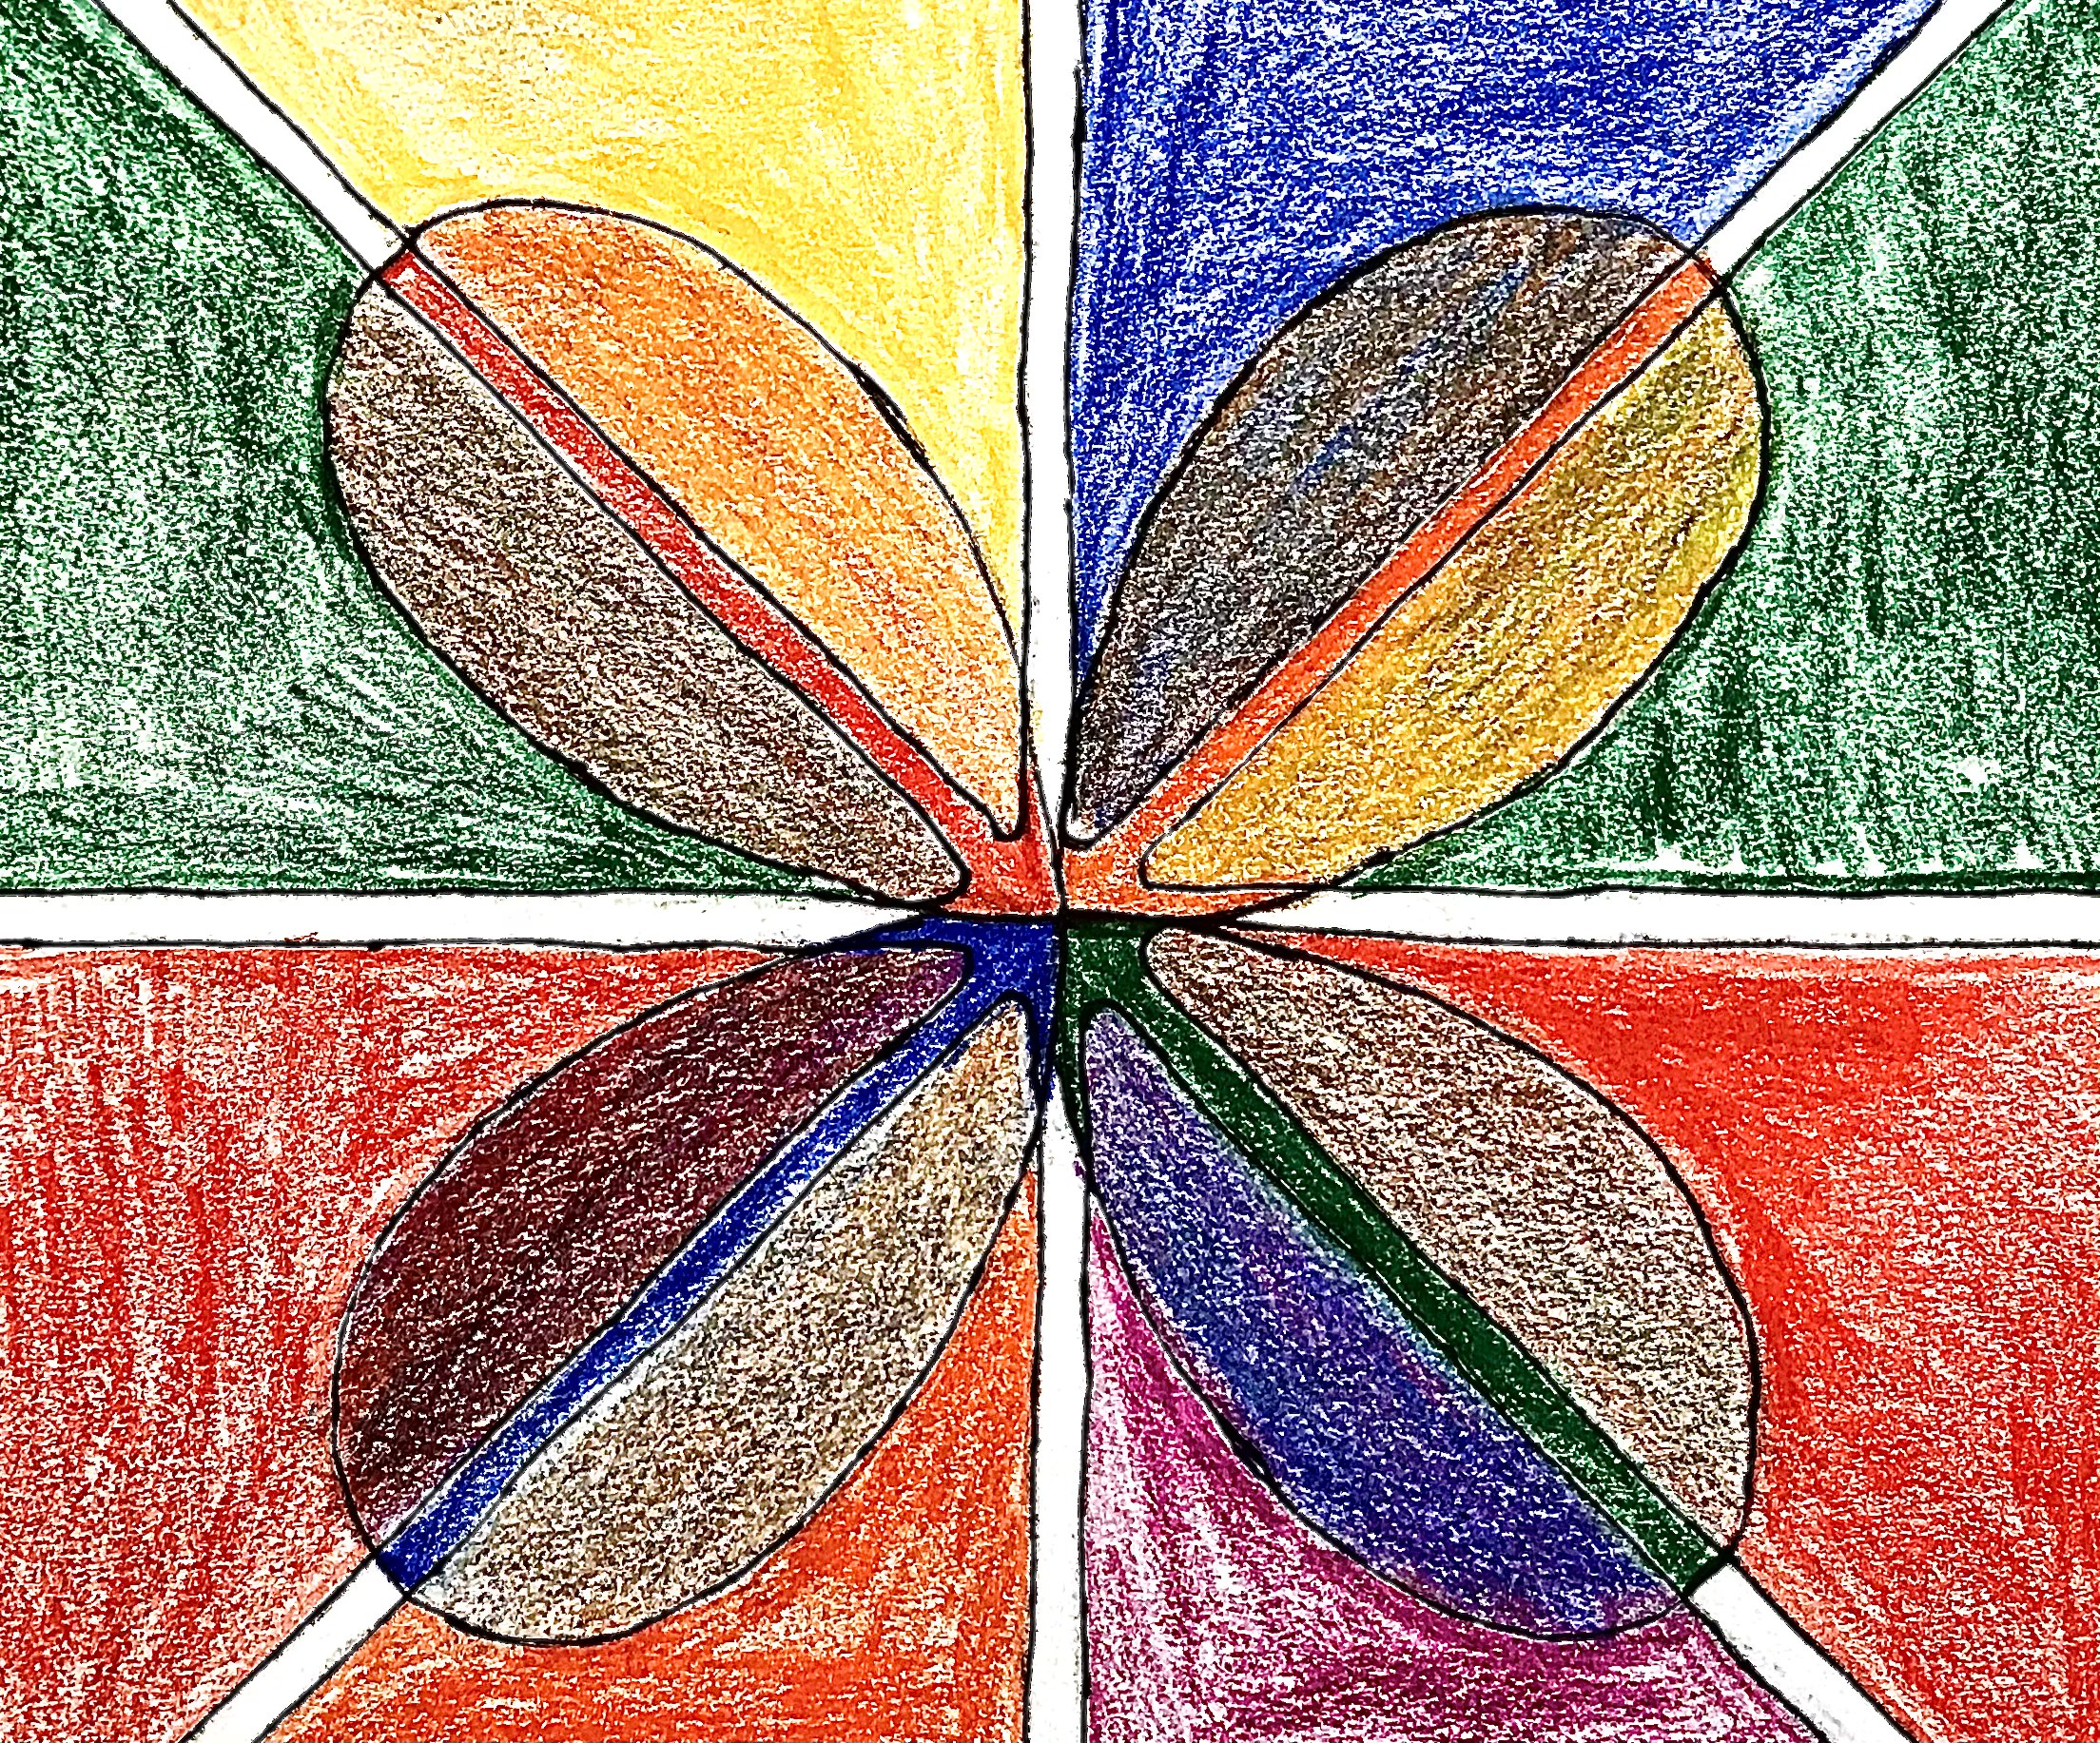
\includegraphics[width=0.9\textwidth]{kauffman_final_art.jpg}

\noindent
\textbf{Introduction}

When I began to play around with polar equations at the beginning of this project, the polar curve
\begin{align*}
    r = \frac{1}{\sin(4\theta)}
\end{align*}
was the first curve that really caught my eye. Artistically, the curve is appealing because of its eight distinct ``parts'' that all radiate from the origin/pole.\footnote{Later in the write-up, I refer to these ``parts'' as ``shards''.} When looking at the graph for this curve, it’s almost as if one can either focus on the eight ``parts'' of the curve---which look like shards that angle towards the origin, hit a radius length of 1, and fly back to the outer depths of the graph---or, one can see the distance between the shards, which look like rays of mathematical validity---eight sunbeams, each one devoted to never dividing by zero.

However, the curve is just as interesting mathematically as it is artistically. Firstly, the graph has asymptotes at any $\theta$ value that would cause $\sin(4\theta)$ to equal zero, because if $\sin(4\theta)$ were equal to zero, then the equation would produce an undefined value. These values of $\theta$ that the curve excludes are $0$, $\nicefrac{\pi}{4}$, $\nicefrac{\pi}{2}$, $\nicefrac{3\pi}{4}$, $\pi$, $\nicefrac{5\pi}{4}$, $\nicefrac{3\pi}{2}$, and $\nicefrac{7\pi}{4}$. You may notice that these are eight values in total. This is the reason why there are eight ``shards'' to the curve. Another interesting part about this curve is that the equation never has an $r$ value smaller than 1. This is because for that to happen, the output of $\sin(4\theta)$---the denominator of the equation---would need to be greater than one. This is impossible because $\sin(4\theta)$ depicts the unit circle with a radius of one.

To complement this graph, I wanted to find a curve that intersected large parts of the ``shards'' of the $r = \nicefrac{1}{\sin(4\theta)}$ graph. The curve
\begin{align*}
    r = 10\sin(2\theta)
\end{align*}
did this. This curve intersects all eight of the parts of the $r = \nicefrac{1}{\sin(4\theta)}$ graph, resulting in 16 intersections. To make it even more interesting, only 8 of these intersections are real solutions. The reason for this is that during the intervals of $\theta = (\frac{\pi}{4}, \frac{\pi}{2}), (\frac{3\pi}{4}, \pi), (\frac{5\pi}{4}, \frac{3\pi}{2}), and (\frac{7\pi}{4}, 2\pi)$, the value of $r$ for $r = \nicefrac{1}{\sin{4\theta}}$ is negative, which flips the points 180 degrees about the origin. An example is an \begin{wrapfigure}{l}{0.55\textwidth}
    \centering
    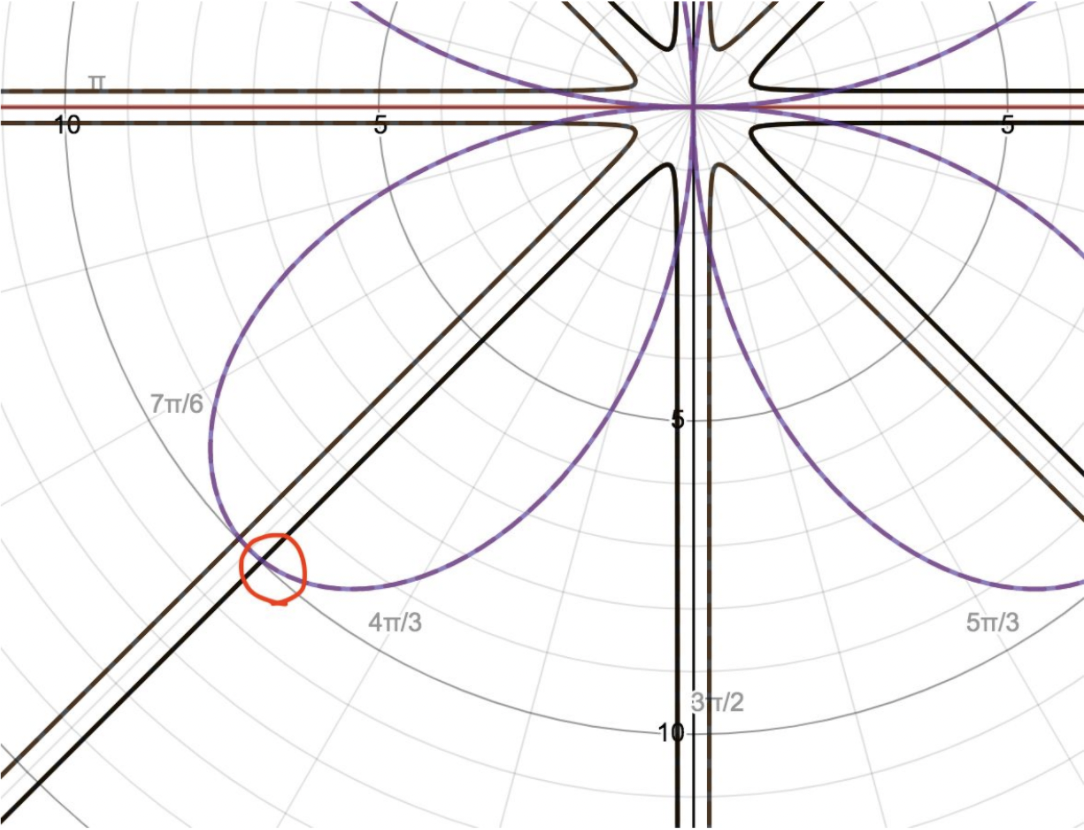
\includegraphics[width=0.55\textwidth]{kauffman_desmos_1.png}
\end{wrapfigure} intersection point in the third quadrant, as seen on the left. $r = \nicefrac{1}{\sin{4\theta}}$ intersects this point shortly after $\theta = \nicefrac{\pi}{4}$ because this leads to a negative $r$ for $r = \nicefrac{1}{\sin{4\theta}}$. However, $r = 10\sin(2\theta)$ intersects this point shortly after $\theta = \nicefrac{5\pi}{4}$, meaning that they do not intersect the point at the same time---not a solution.

This means that, going counter-clockwise around the polar graph, there will be two solutions, then two non-solution intersections, then two solutions, etc. I was able to verify this by looking at the graphs of $y = \nicefrac{1}{\sin{4\theta}}$ and $y = 10\sin(2\theta)$ \begin{wrapfigure}{l}{0.15\textwidth}
    \centering
    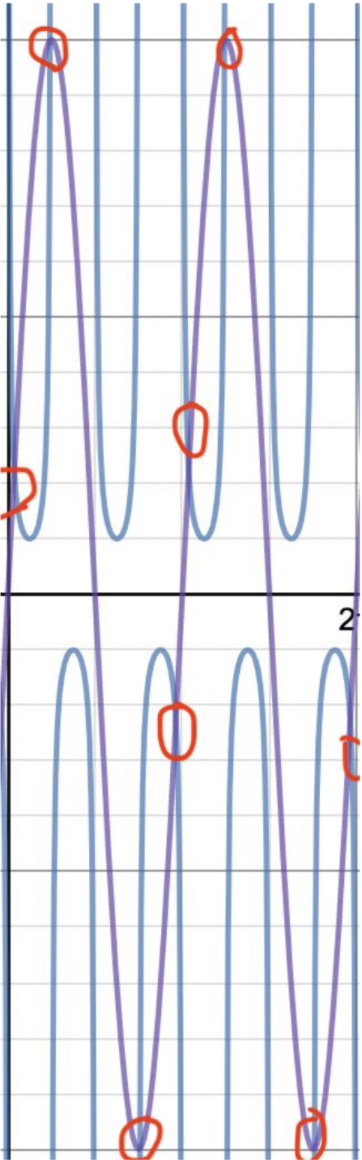
\includegraphics[width=0.15\textwidth]{kauffman_desmos_2.png}
\end{wrapfigure} in Desmos, as seen on the left. We know this graph will only give real solutions at points of intersections because we are graphing the functions in the Cartesian plane, replacing $r$ with $y$. In the Cartesian plane, there is no ambiguity---an intersection is always a solution. From this graph, we can see that there are 8 solutions in the period of $0$ to $2\pi$ (after that, the solutions begin repeating). The eight solutions are $(0.114, 2.266)$, $(0.76, 9.987)$, $(2.318, -9.987)$, $(3.027, -2.266)$, $(3.256, 2.266)$, $(3.902, 9.987)$, $(5.523, -9.987)$, and $(6.169, -2.2657)$.
\\\\
\noindent
\textbf{Attempting to Find an Analytical Solution}

Before I cover how I represented these solutions with color, I would like to present my attempt to solve this analytically, not using Desmos. First, I set
\begin{align*}
    \frac{1}{\sin{4\theta}} = 10\sin{2\theta}.
\end{align*}
Then, I defined a variable $t = 2\theta$. The equation now looked like \begin{align*}
    \frac{1}{\sin{2t}} = 10\sin{t}.
\end{align*}
Then, because $\sin{2a} = 2\sin{a}\cos{a}$, I made the equation
\begin{align*}
    \frac{1}{2\sin{t}\cos{t}} = 10\sin{t}.
\end{align*}
Next, I cross-multiplied to get
\begin{align*}
    20\sin^2{t}\cos{t} = 1,   
\end{align*}
and then
\begin{align*}
    \sin^2{t}\cos{t} = \frac{1}{20}.   
\end{align*}
Then, because $\sin^2{a} = 1 - \cos^2{a}$, we can write
\begin{align*}
    \left(1 - \cos^2{t}\right)\cos{t} = \frac{1}{20}   
\end{align*}
and
\begin{align*}
    \cos{t} - \cos^3{t} = \frac{1}{20}.   
\end{align*}
This is when I hit a roadblock and couldn't think of anything to do since the cosines have different exponents.

\noindent
\textbf{Coloring the Graph}

Now, when it came time to depict the intersections with color, I wanted to represent the non-solution intersections by using the blackish-brown result of mixing two complementary colors and the solutions by using a more pleasant mix of two primary or secondary colors.

There are four ``leaves'' of the $r = 10\sin{2\theta}$ equation, and I made two opposing leaves red and green (complements) and the other two opposing leaves orange and blue (complements). Now, if the ``shard'' of the $r = \nicefrac{1}{\sin(4\theta)}$ intersected with one of the four leaves and was not a solution, I colored the ``shard'' the complement of the leaf, which is the color of the opposing leaf. When the ``leaf'' and the ``shard'' overlapped, a brownish color formed, signifying that their intersection was not a solution to the equation.

However, if the intersections between the two equations were solutions, I wanted the color formed to be a pleasant primary or secondary color. I applied a system of choosing the color of the ``shard'' in this scenario so that the color progression would have some sort of order. The system was that, in a color wheel of only primaries and secondaries, I took the color of the leaf---the $r = 10\sin{2\theta}$ equation---and I went two spaces clockwise in the color wheel and made that the color of the shard---the $r = \nicefrac{1}{\sin(4\theta)}$ equation. When I did this, the color in between the color of the ``shard'' and the color of the ``leaf'' in the color wheel would form when the ``shard'' and ``leaf'' overlapped. For example, when there was a red leaf, I made the ``shard'' yellow, and that made the space where they intersected orange. When there was a blue leaf, I made the ``shard'' red, and that made the intersection space violet.

This ended up giving some sort of pattern to the space where there were solutions, yet I must acknowledge the shortcomings of this method. It is not very clear where the intersections are from the way I did it. All you can really see is that the two functions sometimes form a brown color in the space where they intersect, and they sometimes form a different, more pleasant color; the actual points of intersection are not highlighted at all. From my perspective, this is its greatest limitation; however, I do believe that my polar art effectively contrasts the areas of intersection that are solutions with the areas of intersection that are not solutions.
 


\newpage

\nnarticleheader{Putting a Spin on the Average Bike}{Jaiden Shuchman, Jay Crowther, and Ryan Davey, Haverford '23}
In 2018, Denise Mueller-Korenek rode a bicycle at 183.9 mph, shattering the previous world record set by Fred Rompelberg, which was 166 mph. Mueller-Korenek accomplished this not only by riding in the slipstream of a drag racer, but by using a custom bike.  Mueller-Korenek’s bike contained extra gears. These gears allowed her to reach her incredible record-breaking speeds. Mueller-Korenek’s unique bike led us to the question: how much do  extra gears affect the speed at which the tires rotate?

Immediately, we understood that a combination of the gears, rpm of the wheels, and the size of the wheels would determine the speed of the bicycle. Investigating this concept presented  many challenges, so we decided to explore only two variables: the number of gear systems and  the ratio of the cog sizes. These values would affect the rpm of the wheels. The speed was not part of our investigation, however, by using the size of the wheels as well as the rpm, velocity  was easily calculated. We used the dimensions of Mueller-Korenek’s bicycle to find the increase in rpm to the bicycle with the addition of more gear systems. We were forced to make logical assumptions for some dimensions of the bike because they were not provided. The image to the left is our quick sketch of the additional gear systems and features a chart to record the top  speeds from the different systems. 

Once we established our main hypothesis, that the addition of gears would increase the rpm of the wheels linearly, we began the mathematical portion of the project. The first step was to figure out the angular velocity and overall metrics of the bike used by Mueller-Korenek.

The equation for angular velocity is the amount of revolutions divided by the time, measured in revolutions per minute. First, knowing that the diameter of the tire was equal to 17 inches, we deduced that the radius would be half that: 8.5 inches. By using the equation for circumference, $C=2 \pi r$, we found that the distance traveled in a full revolution of the tire is roughly 53.4 inches, or $17\pi$ inches. Mueller-Korenek traveled a maximum speed of 183.9 mph, and there are 63360 inches in a mile. With this information, we then multiplied 63,360 by 183.9 to get approximately 11,651,904, which is Mueller-Korenek’s speed converted to inches per hour. We can now divide this by the circumference of the wheel to get the revolutions per hour and we get about 218,200 revolutions per hour. Divide this by 60 to get around 3,638  revolutions per minute.\footnote{Alternate Method: $184=17 \pi r$; $r$ equals revolutions, and 17$\pi$ is the circumference of the wheel. 184 is the maximum speed of the bike. In this equation, you find the number of revolutions in a single hour. By converting the 184 miles into feet, and the 17$\pi$ inches into feet, you are left with $971520=4.4505r$. Then solve for $r$. The following number is the rotations per hour. Divide by 60 to find the rpm, which is 3638.}

$$
\frac{183.9 \text{ mi}}{\text{ hr}} \times \frac{63,360 \text{ in}}{\text{ mi}} \times \frac{1 \text{ rev}}{17\pi \text{ in}} \times \frac{1 \text{ hr}}{60 \text{ min}} = 3,638 \text{ rpm}
$$

The bike tire is attached by an axle to a 12 cog wheel which in turn is connected to a 60 cog wheel by a 55 inch chain.\footnote{This is also an approximation from an average bicycle}
The ratio of 12 to 60 is equivalent to a 1 to 5 ratio. Therefore, we can divide the amount of revolutions by 5 to get the rpm of the 60 cog wheel because it will have to travel 5 times the distance of the chain to accomplish 1 full revolution. 

At Mueller-Korenek’s maximum velocity of 183.9 mph, the 60 cog wheel will be moving at a rate of 727.6 rpm. However, that 60 cog wheel is connected by another axle to a 12 cog wheel, which in turn is connected by a 55 inch chain to another 60 cog wheel.\footnote{This is also assumed.} 
We can do the same math as above, by finding the ratio of 12 to 60 and then dividing, and we get approximately 145.52 rpm for that final 60 cog wheel at Mueller-Korenek’s max speed. That 60 cog wheel is connected directly to the pedals, meaning that she is pedaling at an average of 145.52 rpm. For every time she pedals, her back wheel is turning approximately 25 times.

\begin{align*}
\frac{60}{12} &= 5 \\
\frac{727.6 \text{ rpm}}{5} &= 145.52 \text{ rpm} 
\end{align*}

As we know based on our data, each additional cog with a 60 to 12 ratio yields approximately 5 times as many revolutions per minute of the tires. This is an exponential increase which is proportional to the number of cogs added (starting from 0 gears). This can be modeled after $5^{x}$ because each successive cog will multiply the speed by 5. The equation of this function is $y=145.52(5^{x})$,\footnote{https://www.desmos.com/calculator/opplgoh8i1} where the amount of gear systems with the pedals themselves being 0 is equal to $x$. We are assuming that she is pedaling at a constant speed of 145.52 rpm. From this graph we can determine that when $x$ equals 0, $y$ equals 145.52. When $x = 1$, $y$ should be equal to roughly 727.6. When $x = 2$, $y$ should be going at roughly 3638. When $x = 3$, $y$ should  be roughly 18190 rpm. 

\begin{align*}
145.52(5^{0}) &= 145.52(1) \\
&= 145.52 \text{ rpm} \\
\end{align*}

\vspace{-10mm}

\begin{align*}
145.52(5^{1}) &= 145.52(5) \\
&= 727.6 \text{ rpm} \\
\end{align*}

\vspace{-10mm}

\begin{align*}
145.52(5^{2}) &= 145.52(25) \\ 
&= 3638 \text{ rpm} \\
\end{align*}

\vspace{-10mm}

\begin{align*}
145.52(5^{3}) &= 145.52(125) \\
&= 18,190 \text{ rpm}
\end{align*}

\vspace{5mm}

\renewcommand{\thefigure}{1}
\begin{figure}[h]
    \centering
    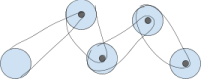
\includegraphics{gears.png}
    \caption{The overall gear pattern at $x=4$}
\end{figure}

If the wheel is connected to the final gear in the sequence, it will be traveling at 90950 rpm, or 4600mph. However, this is pretty much impossible due to the issues of getting to this speed and the fact that no human body or bicycle can withstand this velocity.

Hypothetically, if the bike and rider are indestructible, how many gears do we need to reach the speed of light? The speed of light is 670,616,629 mph, which is equivalent to 13,261,632,213.93 rpm of the wheel with a $17\pi$ inch circumference. Assuming she is pedaling at the same constant speed of 145.52 rpm,  we plugged that very large number in for $y$, solved for $x$, and got 11.38771942. This number is the amount of groups of 60 tooth to 12 tooth gears with 55 inch chains (gear systems), needed to  reach the speed of light if she pedals at the speed she did when she reached 184 mph. Obviously, this is impossible for a number of reasons from friction, to the structural integrity of the bike and rider.  

$$
    \frac{670,616,629 \text{ mi}}{\text{ hr}} \times \frac{1 \text{ hr}}{60 \text{ min}} \times \frac{63,360 \text{ in}}{\text{mi}} \times \frac{1 \text{ rev}}{17\pi \text{ in}} = 13,261,632,213.93 \text{ rpm} \\
$$

\begin{align*}
    145.52(5^{x}) &= 13,261,632,213.93 \\
    5^{x} &= 91,132,711.75  \\
    x &= \log_5 91,132,711.75  \\
    x &= 11.38771942 \text{ gear systems}
\end{align*}

The equation $y=pn^{x}$ can be used to determine the rpm of a bike’s wheels that has a fixed ratio between gear sizes. $p$ is the amount of revolutions per minute of the pedals, $n$ is the ratio of the gears, $x$ is the amount of gear systems, and $y$ is the revolutions per minute of
the wheel. If you multiply $y$ by whatever the circumference of the wheel is, you get the speed of the bike.  

We arrived at this function through a series of logical steps using the data and  dimensions of the initial bike used by Mueller-Koerner. We observed that the wheel attached to  the pedals, or in terms of our equation $x=0$, is spinning at 145.52 rpm.  Therefore, $y=145.52$ rpm. Following this discovery for the first gear system, the gear was spinning at 727.6 rpm, a jump by 5 times greater than the previous value. The wheel itself was spinning at roughly 3638 rpm, which once again, is 5 times faster than the previous gear. This showed us that each gear roughly had a 1:5 ratio with the successive gear; at this point, we realized that this meant each consecutive gear multiplied the previous gear’s speed by 5, so this meant it could be modeled by a transformation of the function $5^{x}$. Now, using prior knowledge, we understood that when $x=0$, the $y$-value had to be equal to 145.52. This is the rpm of the pedals initially. We then determined that the only way to achieve this with a transformation  of our function was to multiply $5^{x}$ by this number, leaving us with the equation $145.52(5^{x})$. From this, we can determine that the number multiplied by $5^{x}$ (which is denoted by the variable $p$) is always the amount of revolutions per minute of the pedals (essentially, this is the angular velocity  of the first gear). Also, we can confirm that the base 5 (denoted by $n$ in our equation) is the ratio  from each gear to the successive one, making $n$ the growth factor for the speed.  
From this equation, we can see that it is theoretically possible, with an indestructible bike and a sufficient force to pedal the bike and hold itself together, it is possible to go infinitely fast.  We multiply the output of the wheels by 5 every time a gear system is added (in the event that the gear system is the same as Mueller-Korenek’s), so it is an exponential growth. 

To further prove the validity and accuracy of our function, we used the dimensions from another familiar bike: Mr. Bridge’s 20 speed bike. All of these calculations were performed  assuming there is no outside force acting upon this bike when in motion (e.g. air resistance and  friction) and that Mr. Bridge is strong enough to pedal at any speed he pleases. The radius of the tires is 14 inches, therefore making the circumference $28\pi$ inches. Following this, we counted the teeth on each gear, resulting in the values 52 and 11 for their respective gears. We then calculated  the gear ratio (by dividing these numbers) to be approximately 4.7272. We now have enough  information to plug these values into our equation and set up the problem.  

We assumed that Mr. Bridge was pedaling at 100 rpm, a high number,  but as we stated previously, strength is no concern for Mr. Bridge. Our equation, with the inserted values, was $y=100(4.7272^{1})$: Mr. Bridge’s bike possessed only a single gear system,  so $x$ can be substituted with the value 1. After solving this equation, we get $y=472.72$ rpm.  If we multiply this number by the circumference of the wheel, that being $28\pi$ or 87.962, we can  find the linear velocity. This ended up being equal to 41581.4 inches per minute. We converted this to 2494883.8 inches per hour by multiplying the previous value by 60. Then, we divided this by 63360 (the number of inches in one mile) to get a value of 39.376 miles per hour.  This value is how fast Mr. Bridge would be going if he pedaled at an angular velocity of 100 rpm and was in the highest gear possible for his bike. This result is realistic and makes sense given that Mr. Bridge is unable to pedal 100 rpm in real life, so his real speed would be less based on air resistance, friction, and a lack of strength.  

\begin{align*}
y=100(4.7272^{1}) \\
= 472.72 \text{ rpm} 
\end{align*}

$$
\frac{472.72 \text{ rev}}{\text{min}} \times \frac{28\pi \text{ in}}{\text{rev}} \times \frac{60 \text{ min}}{\text{hr}} \times \frac{1 \text{ mi}}{63360 \text{ in}} = 39.376 \text{ mph}
$$

In reflection, we learned that our hypothesis, that if more gear systems were added then  the rpm of the bike would increase linearly, was wrong. It turned out that the addition of extra gear systems would result in an exponential increase in rpm. After watching the video of Californian biker Denise Mueller-Korenek breaking the world record of the top speed traveled on  a bike, we weren’t very moved. However, what caught our attention was the bike Mueller-Korenek used to do so. Seeing the extra gear systems on her bike we had a million  questions, most of which being ridiculous. One question that stuck though, was to what degree did the gears affect the speed of her bike? After our research we learned just how powerful the addition of extra gears are. It’s truly mind boggling when you see something so small have such  an insane amount of repercussions. Small things tend to make huge differences, whether you  expect it or not. 

\pagebreak

\noindent

\begin{thebibliography}{4}
\bibitem{openstax} 
“10.2 Kinematics of Rotational Motion - College Physics.” OpenStax,  
openstax.org/books/college-physics/pages/10-2-kinematics-of-rotational-motion.  

\bibitem{chappel}
Chappell, Bill. “Woman Rides Bicycle To 183.9 MPH - A World Record.” NPR, NPR, 18 Sept.  2018,  
www.npr.org/2018/09/18/649221471/woman-rides-bicycle-to-183-9-mph-a-new-world-record

\bibitem{stout}
Stout, James. “The Crazy Detail That Went Into Creating This Record-Breaking Bike.” Bicycling , Bicycling, 20 Sept. 2020,  
www.bicycling.com/bikes-gear/a23305843/what-went-into-creating-this-record-breaking-bike/

\bibitem{mbs}
“Table Of Radius Values For Bicycle Sprockets.” Machinehead Bike Software,  
\url{www.machinehead-software.co.uk/bike/chain_length/sprocket_radius_table.html}

\end{thebibliography}


\newpage

% Begin the applied science section
\nnwallpaper{2021_Applied_Science_Page_Border.pdf}
\def\currentTitleWallpaper{2021_Applied_Science_Title_Page_Border.pdf}

\addcontentsline{toc}{part}{Applied Science}
\nnimagepage{2021_Applied_Science_Section_Title.pdf}

\nnarticleheader{Exploring Symmetry in Quantum Physics}{Brian Williams, Haverford '21}

\noindent
\textbf{Introduction}

Humanity has always been drawn to symmetry, both in nature and in the structures we build ourselves. Perhaps our brains are wired to see beauty in symmetry, or maybe we just find practicality in order. Regardless of our reasons for liking symmetry, it seems that nature itself has its own affinity for it. Some symmetries arise naturally from the laws governing our universe, and some seem to give rise to laws of their own---especially in quantum physics. 

But what exactly \emph{is} symmetry? What does it mean for a system to be symmetrical? Well, an object has a symmetry if when you do something to it---move it, turn it, flip it---it looks the same after you're done with it. For example, a butterfly looks symmetrical because when you reflect it across its $y$-axis, it's hard to tell that anything has changed. More specifically, it has a particular \emph{symmetry corresponding to that transformation}.

As a more detailed example, consider a hydrogen atom, a system with just a proton and an electron. The proton is much heavier than the electron, so we really only need to consider the electrostatic potential on the latter, which generates a force that pulls the electron towards the proton. The potential energy is inversely proportional to the distance between the two particles, meaning that we can write it as $V(r)$, where $r = \sqrt{x^2 + y^2 + z^2}$, as opposed to $V(x, y, z)$. This property gives rise to an interesting symmetry of the system: if we rotate the electron around the origin, the value of the potential shouldn't change. After all, it only depends on the distance to the origin. For instance, a $90^{\circ}$ rotation around the $z$-axis involves the substitutions
\begin{align*}
    x &\rightarrow -y \\
    y &\rightarrow x \\
    p_x &\rightarrow -p_y \\
    p_y &\rightarrow p_x
\end{align*}
where $x$, $y$, and $z$ are the position variables, and $p_x$, $p_y$, and $p_z$ are the momentum variables (since we rotated around the $z$-axis, $z$ and $p_z$ are left unchanged):
\begin{align*}
    r &= \sqrt{(-y)^2 + (x)^2 + z^2} \\
    &= \sqrt{x^2 + y^2 + z^2}.
\end{align*}
Its form is unchanged---and you would find the same with any other rotation around the origin. In other words, the system has some sort of rotational symmetry.

But what about the changes in $p_x$ and $p_y$? Since we looked at the potential energy, we might as well do the same to the kinetic energy
\begin{align*}
    T = \frac{p_x^2 + p_y^2 + p_z^2}{2m}
\end{align*}
which upon plugging in the two momentum variable substitutions we didn't use before, we find is also invariant. By contrast, if we'd had a transformation like $p_x \rightarrow 0$, then there would be a clear difference in the behavior between the original and transformed systems. So in order to analyze the effect of a transformation on a system, we need to consider both the kinetic energy $T$ and potential energy $V$. Here's one useful way to do this, using an object called the \emph{Hamiltonian}:
\begin{align*}
    \mathscr{H} = T + V.
\end{align*}
It's really just a fancy name for the sum of the total kinetic and potential energy. Despite its seemingly simple form, it contains all the information about how a system behaves, or changes over time.\footnote{Classically, one can use a set of equations called the \emph{canonical equations} to do this. This is called the \emph{Hamiltonian formalism}, as opposed to the Newtonian approach which uses Newton's three laws, including $F = ma$, to figure out how a system behaves.} So here's the key point: when a transformation leaves the Hamiltonian invariant, the \emph{behavior of the system} is left invariant.

\noindent
\textbf{Transformations in Quantum Mechanics}

In order to examine transformations in quantum mechanics---which are a bit more abstract than just substituting variables---we'll need some notation. Let $A$ be some abstract transformation, which we could apply to some abstract object represented by the symbol $|v\rangle$ (pronounced ``ket v''). For example, $A$ could be the rotation of some object by 90 degrees (about the $z$-axis) and $|v\rangle$ could be the butterfly we were talking about before. After being acted upon by the rotation $A$, the butterfly will end up in a new rotated state $|v'\rangle$:
\begin{center}
    \centering
    \begin{minipage}{0.4\textwidth}
        \centering
        \begin{tikzpicture}
            \draw[black, thin] (-0.4\textwidth,0) -- (0.4\textwidth,0);
            \draw[black, thin] (0,-0.4\textwidth) -- (0,0.4\textwidth);
            \node (butterfly) at (0,-0.035\textwidth) 
            {
\includegraphics[width=.45\textwidth]{williams_butterfly.png}};
            \node (ket) at (0.25\textwidth, 0.25\textwidth) {$|v\rangle$};
        \end{tikzpicture}
    \end{minipage}
    \begin{minipage}{0.1\textwidth}
        \centering
        \begin{tikzpicture}
            \draw[black, thick, ->] (-0.5,0) -- (0.5,0);
            \node at (0, 0.3) {$A$};
            \node at (0, -0.4) {};
        \end{tikzpicture}
    \end{minipage}
    \begin{minipage}{0.4\textwidth}
        \centering
        \begin{tikzpicture}
            \draw[black, thin] (-0.4\textwidth,0) -- (0.4\textwidth,0);
            \draw[black, thin] (0,-0.4\textwidth) -- (0,0.4\textwidth);
            \node (butterfly) at (0.03\textwidth,0)
            {
\includegraphics[width=.45\textwidth, angle=90]{williams_butterfly.png}};
            \node (ket) at (0.25\textwidth, 0.25\textwidth) {$|v'\rangle$};
        \end{tikzpicture}
    \end{minipage}
\end{center}
To show this relation, we write
\begin{align*}
    A|v\rangle = |v'\rangle.
\end{align*}

This bracket-based notation, quite imaginatively called bra-ket notation, is common in quantum mechanics.\footnote{I might as well add that there's another symbol called a ``bra'' which looks like $\langle v|$. If you're familiar with linear algebra, $\langle v|$ is the conjugate transpose of $|v\rangle$.} We haven't really defined what $A$ and $|v\rangle$ mean mathematically, but for these purposes it's probably better to think of them just in terms of what they represent: a transformation and an object being transformed. Formally, $A$ is called an \emph{operator} and $|v\rangle$ is actually a \emph{vector}.\footnote{But try not to think of $|v\rangle$ as a vector like an arrow in space, like you usually do.} In quantum mechanics, a \emph{statevector} like $|v\rangle$ or $|\psi\rangle$ represents a particular state of the system (the Greek letter $\psi$ ``psi'' is most commonly used for some arbitrary state). For example, $|\psi_0\rangle$ could represent an electron bound to a proton, while $|\psi_1\rangle$ could represent the same electron that just got released some time later.

Before moving on, I'd like to emphasize the difference between the dynamics of a system and a particular state of a system. When we considered the rotation of the hydrogen atom, we looked at a symmetry of the \emph{dynamics} of the system. The Hamiltonian didn't change, so the electron still moves in the same way we'd expect. But (if we imagine the electron as a classical particle with definite position) the position of the electron still changed after the rotation. In quantum mechanics, the dynamics of the whole system itself are represented by some Hamiltonian \emph{operator} $H$, similar in structure to the Hamiltonian function $\mathscr{H}$ we looked at before. An isolated hydrogen atom has some particular $H$ which dictates how the system changes over time. On the other hand, the state of the system $|\psi\rangle$ will change over time depending on $H$. As we will see, however, we can look at how a statevector is affected by transformations to reveal transformations regarding the dynamics of the whole system.

Now we have the tools we need to analyze transformations in quantum mechanics. Some examples of transformations you've probably seen are spatial translations, rotations, and reflections, as mentioned above. We can use specific operators for these, like $T(\mathbf{a})$ (to translate the state by the vector $\mathbf{a}$), $R_x(\theta)$ (for a rotation by $\theta$ around the $x$-axis), and $\Pi$, respectively. The $\Pi$ operation is commonly called a \emph{parity} transformation. Here's an example of what a translation operator would look like for a one-dimensional system, where we only consider the $x$-direction:
\begin{align*}
    T(a)|x\rangle = |x+a\rangle
\end{align*}
where $|x\rangle$ is a state with a well-defined position at $x$. Classically, this would mean doing
\begin{align*}
    x \rightarrow x+a.
\end{align*}
To describe a series of transformations, let's say a translation first and then a rotation, we would write $R_x(\theta)T(\mathbf{a})|\psi\rangle$, where the operators closest to $|\psi\rangle$ act first.

We can also consider transformations involving time, such as moving forward or backwards in time $U(t)$---we'll call this \emph{time evolution}---or reversing time similar to the parity transformation ($t \rightarrow -t$), called \emph{time-reversal}. To represent a state at time $t=0$, we write $|\psi(0)\rangle$
\begin{align*}
    U(t)|\psi(0)\rangle = |\psi(t)\rangle
\end{align*}

The operators $H$ and $U(t)$ are very closely related---as mentioned before, the Hamiltonian contains the information about how a system behaves, so it makes sense that it'd be tied to an operator $U(t)$ that moves the system forwards in time. It's pretty common to be given a Hamiltonian and use it to find $U(t)$, in the same way that you might be given the forces or potentials in a classical system and use Newton's laws to find the equations of motion.

Consider the symmetries coming from these transformations. The translation, rotation, and time evolution operators are controlled by a specific parameter, meaning that they are \emph{continuous}. You can choose how much you'd like to move, rotate, or evolve a state. By contrast, the parity and time-reversal transformations are \emph{discrete}. We saw that our mirrored butterfly had a discrete symmetry. What about the hydrogen atom? Well, since it didn't matter how much we rotated it, it seems to have a continuous symmetry.

Now that we have this notation, there's a much easier way to write that a system with a Hamiltonian $H$ has a certain symmetry, let's say under a transformation $A$. Let's say we have a state $|\psi\rangle(0)$ at time $t=0$ and let it change over time. This change depends on $U(t)$, which in turn depends on the Hamiltonian $H$:
\begin{align*}
    U(t)|\psi(0)\rangle = |\psi(t)\rangle.
\end{align*}
Now let's imagine a different scenario, where we had transformed our state according to $A$ at $t=0$ and \emph{then} let it change over time:
\begin{align*}
    U(t)A|\psi(0)\rangle = A|\psi(t)\rangle.
\end{align*}
Since the system is symmetrical under $A$, there shouldn't be any difference in how the states changed over time---the system still behaves in the same way. In other words, the two end results, $U(t)|\psi(0)\rangle$ and $U(t)A|\psi(0)\rangle$, should only differ by a transformation on the former:
\begin{align*}
    AU(t)|\psi(0)\rangle = U(t)A|\psi(0)\rangle.
\end{align*}
But since this is a symmetry of the system, not this particular state, we only need to write
\begin{align*}
    AU(t) = U(t)A
\end{align*}
to mean that our system has a symmetry corresponding to $A$.

Although it might be tempting to think that $AU(t) = U(t)A$ no matter the scenario, this isn't always the case. All natural laws, like the electromagnetic, weak nuclear, and strong nuclear forces, are invariant under space and time translations. The weak force, however, isn't invariant under parity transformations. This force is responsible for radioactive beta decay. In 1956, physicist Chien-Shiung Wu performed an experiment with the following beta decay in cobalt-60:
\begin{align*}
    ^{60}\text{Co} \rightarrow\: ^{60}\text{Ni} + e^- + \Bar{\nu}
\end{align*}
where $e^-$ is an electron and $\Bar{\nu}$ is an antineutrino. She found that the electrons had a preferred direction in which they'd decay, opposite the spin $^{60}\text{Co}$, leading to the conclusion that parity symmetry was \emph{violated}. So although this is a situation in which there's a lack of symmetry, this actually helps us understand the universe better---nature treats a completely mirrored version of the universe differently than a non-mirrored one, contrary to what you might expect.

\noindent
\textbf{Conservation Laws}

In 1918, mathematician Emmy Noether proved a theorem linking continuous symmetries to \emph{conserved quantities}. A conserved quantity is one that doesn't change over time---for example, if the momentum of a system is conserved, then the system should have the same momentum after waiting for a little while:
\begin{align*}
    \frac{dp}{dt} = 0.
\end{align*}
This theorem, which applies to both classical and quantum systems, is extremely important in explaining the correspondence between the symmetries and behaviors of a system.
\begin{theorem}[Noether's theorem]
Every continuous symmetry in a system corresponds to a conserved quantity.
\end{theorem}
Here are the relationships from the continuous symmetries we've looked at:
\begin{center}
    \begin{tabular}{|c|c|c|}
    \hline
    Transformation & Operator & Conserved quantity \\
    \hline
    Translation & $T$ & Momentum \\
    Rotation & $R$ & Angular momentum \\
    Time evolution & $U$ & Energy \\
    \hline
    \end{tabular}
\end{center}
The first two might look like they make sense, but the third isn't immediately obvious. But remember that the Hamiltonian---the total energy of the system---dictates the behavior of the system over time.

Since our hydrogen atom had rotational symmetry, we can use Noether's theorem to reason that if the system isn't tampered with, the angular momentum of a state shouldn't change over time. This is a nice way to skip some calculations, but it's also possible to go the other way: it's possible to take a variable, like position or energy, and derive, or \emph{generate} a transformation operator from it. Variables in quantum mechanics like position and momentum also happen to be represented by operators, such as $X$ and $P$, which can be used to generate the translation and rotation operators. We won't go into the details since that gets into some technical linear algebra, but just knowing the relationship between symmetries and conserved quantities is a key part of understanding symmetries in quantum mechanics and physics in general.

\noindent
\textbf{Energy Levels}

For a system with a Hamiltonian $H$, there are certain states $|E\rangle$ with definite energies $E$:
\begin{align*}
    H|E\rangle = E|E\rangle
\end{align*}
where $E$ is a number (but $H$ is an operator, like before). In general, a system could have discrete or continuous energy levels, or possibly both. From chemistry, for example, you'll remember that the electrons in an atom can occupy different discrete energy levels, and that photons can excite them to higher levels. The above equation can be solved to find these specific energies and states, but sometimes the Hamiltonian for a system can be extremely complicated---even for a helium atom, there are no exact solutions for $|E\rangle$. Instead, physicists must use approximations.

One common approach is to write the Hamiltonian as a sum of terms:
\begin{align*}
    H = H_0 + H_p.
\end{align*}
Remember that the Hamiltonian is just the kinetic plus the potential energy, so adding two Hamiltonians together just means introducing more kinetic or potential energy terms to our system (but an added Hamiltonian doesn't have to include another kinetic/potential term if we already have it included). If we wanted to analyze the helium atom, we could use $H_0$ to represent the attraction of the electrons towards the nucleus and $H_p$ for the electron-electron interaction. In general, $H_p$ could either be an approximation to the system we'd be trying to solve, or a physical external change to our system, like if we turned on a small magnetic field to disturb the atom, since this would introduce a new potential.

Here's where symmetry properties come into play: we can use them to figure out \emph{how the energy levels split} when we apply this $H_p$ term, called a $perturbation$. Let's say we have a system with multiple states $|E_1\rangle$ and $|E_2\rangle$ that correspond to the same energy $E$; these states are known as \emph{degenerate}. But it's possible that if we apply a perturbation---which could be us making a mathematical change to fix an approximation, or us actually applying some physical change like a magnetic field---these states in the same energy level might \emph{split} into states each with different energy levels.

When a Hamiltonian is symmetrical under a bunch of related transformations, like the hydrogen atom with any rotation around the origin, it's helpful to classify the set of all the transformations as an object called a \emph{group}. If you imagine rotating an object like a basketball, notice that a series of rotations in succession is always equivalent to some other, single rotation. Also notice that there's always an inverse transformation, namely a rotation that can bring the basketball from a rotated state back to where it was. In order for a set of transformations to be considered a group, it must satisfy those properties (two transformations from the group can be expressed as just one, there always exists an inverse transformation) and more. The group we just gave has an infinite amount of elements, since there are an infinite amount of rotations you could do, but there are also finite groups. Lots of molecules can be flipped or rotated in certain ways and look the same, but not in an infinite amount of ways, like a water or ammonia molecule.

\begin{wrapfigure}{r}{0.25\textwidth}
    \centering
    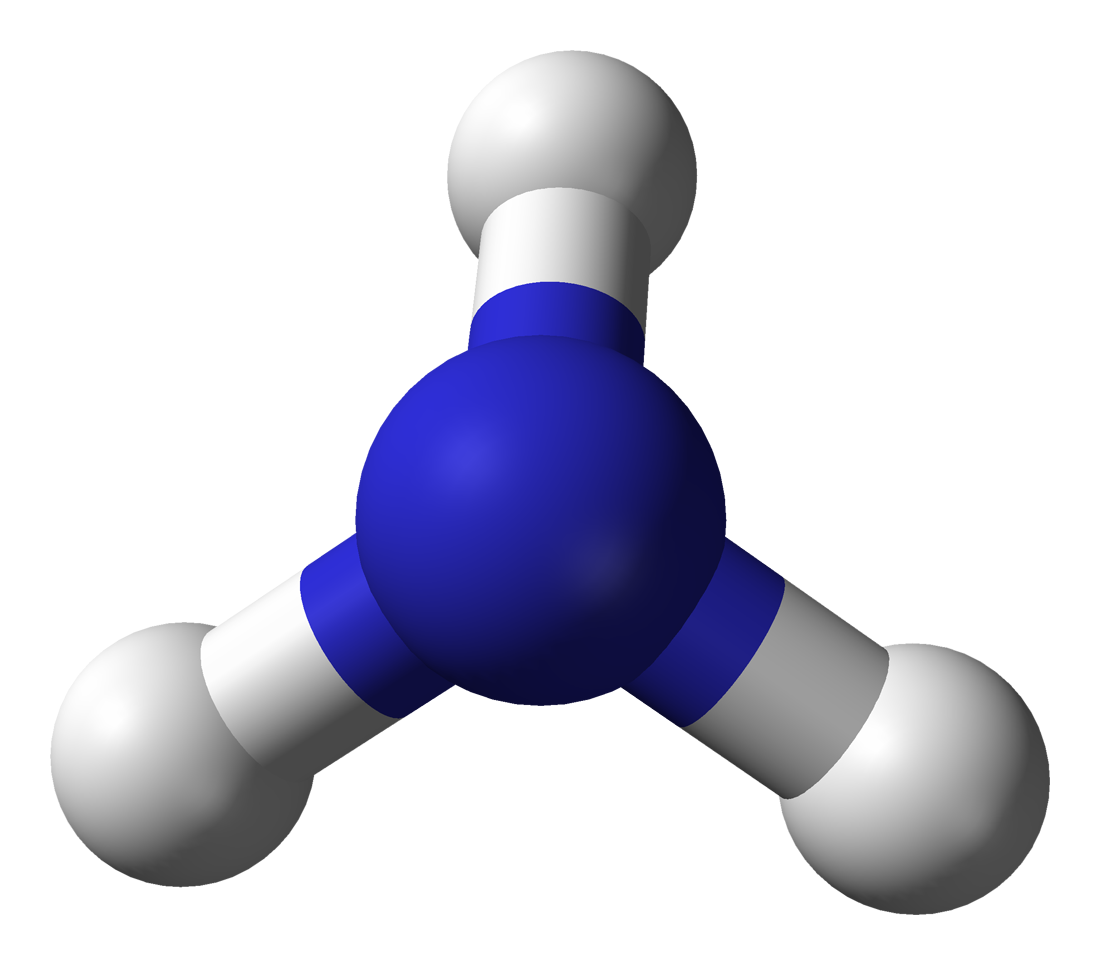
\includegraphics[width=0.2\textwidth]{williams_ammonia.png}
\end{wrapfigure}

It turns out that if a Hamiltonian is symmetrical under a certain group, then all of the states corresponding to one energy level are related to this group through a specific set of matrices, known as a \emph{representation} of the group. By knowing that set of matrices, not only do you have a way to figure out which states might belong to the same energy level, but it's also possible to figure out how much that energy level might split after a perturbation.

\noindent
\textbf{Conclusion}

A lot of the topics here (groups, Hamiltonian mechanics, conservation laws) could be discussed for much longer on their own, but the goal was to give an introduction to the roles they each play in understanding symmetry in quantum mechanics. Groups play a significant role in many aspects of quantum physics from the structure of molecules to the way the operators representing variables behave with each other. They play an even larger role in quantum field theory, to the point where the Standard Model---the theory of elementary particles including the electromagnetic, weak, and strong forces---can be described using a special symmetry group. 

Symmetry laws are valuable because---in contrast to approximations---the information we can derive from knowing the symmetries is \emph{exact}. Understanding symmetry, both in everyday life and in quantum mechanics, can make objects much easier to understand. Symmetries can also help us figure out the underlying laws dictating our world---though as we saw before with Wu's Cobalt-60 experiment, some symmetries can be broken. Interestingly, a theorem called the CPT theorem says that under simultaneous charge conjugation (switching all particles with their antiparticles), parity, and time-reversal, the laws of our universe \emph{shouldn't} change.

Once you've gotten a feel for the role that symmetries play in physics, it's really a matter of wondering why all of these symmetries exist, and why they're so appealing. Artists and architects often use symmetry to guide their works. Physicists often use symmetry to discover the laws governing our world. But do these symmetries appear by chance, emerging out of pure convenience? Or does nature itself, with its most fundamental laws, see the beauty in symmetry?



\newpage

\nnarticleheader{The Beauty of Newton’s First Law of Motion}{Mitav Nayak, Haverford '22}

\noindent
\begin{quotation}
\textit{Every body persists in its state of being at rest or of moving uniformly straight forward, except insofar as it is compelled to change its state by force impressed}
\begin{flushright}
Sir Isaac Newton
\end{flushright}
\end{quotation}

\noindent
\textbf{Introduction}

Above is Newton’s first law as written in 1687 in his book \emph{Principia Mathematica}, translated from his own Latin words; the law that seems to have redefined and refined human understanding of a previously hazy phenomenon: motion. However, while Newton is generally given credit for this discovery, it was really Galileo who first pieced together a clear understanding of motion with his law of inertia. Both laws essentially said the same thing: an object remains at motion or at rest unless acted upon by another force.

While all three of Newton’s laws are brilliant, I find the first to be perhaps the most intriguing. Nowadays, people seem to take the law for granted. We’ve heard it said—in some form or another—since elementary school. At this point, it almost seems \emph{obvious}. But it is not obvious. In fact, I would argue that it is almost counterintuitive: have \emph{you} ever seen an object stay in a state of motion for eternity?

\noindent
\textbf{The History of Motion}

This, the concept of an object staying in a state of motion for eternity, is what I find fascinating. For hundreds of years, physicists and philosophers had attempted to make sense of the concept of motion. Greek philosopher Aristotle was in many eyes one of the first to put forth ideas regarding motion; ideas that lingered for over a thousand years. Aristotle believed that there existed four elements—Earth, Water, Air, and Fire—and that motion was a result of objects attempting to reach their natural place. For example, he argued that smoke rises because it mostly consists of air, rain falls because it consists of water, and a rock falls to reach the Earth. This, I would argue, seems much more intuitive to most people. It’s no wonder the ideas were prevalent for such a long period of time.

When Galileo and Newton came along almost two thousand years later and redefined motion, physics was altered forever. One part of the law, the part that asserts an object will stay at rest unless acted upon, may not have come as too much of a shock to people. It was not necessarily “groundbreaking,” as Aristotle himself had argued something similar. He differentiated “natural motion” (i.e. water falling) with “violent motion,” explaining that motion against an object’s natural state—like picking up a rock from the ground—was the latter. He believed that a heavy rock would stay at rest forever in this “natural” state, unless someone exerted “violent motion” upon it. The other part of Newton’s law, however, was the novel and mind-blowing part, changing how people perceived an object’s “natural state.”

\noindent
\textbf{The Natural State of Motion}

People could not comprehend that an object may persist in a state of motion forever, largely because we do not see it occur on a day to day basis. In our lives, whenever we see an object start moving, it ultimately stops. Galileo and Newton’s discovery that an object could start moving and would naturally never stop seemingly went against real-life observations. But, if we look closely, there are examples of objects persisting—or “wanting” to persist—in a state of motion in real life. For example, when we slide a hockey puck on ice, it will continue skidding along for a long period of time. We know that it will eventually stop, as even the smoothest ice has at least some friction, meaning that there is in fact another force acting on the moving puck. But if we could imagine the puck in a completely frictionless ice rink, the law of inertia suggests the puck would continue in its state of motion for eternity. It would never slow down or stop. Another example of the law is an instance of sudden braking or acceleration in the vehicle. If we are traveling in a car and have to suddenly stop, or hit a brick wall, our body throws itself forward. While the car stops, our body “wants” to stay in its state of motion. If we suddenly accelerate from rest, our body flies backward against our seat, “wanting” to stay in a state of rest.

Before the law of inertia, people believed there was some force acting on an object in motion which caused it to continue moving. They would argue that the moving hockey puck has something acting on it that allows it to propel itself forward. It was hard to understand that, just like a still hockey puck will not move unless something impels it to, a moving hockey puck on frictionless ice will not stop unless something impels it to do so. While the law may seem obvious to us now, it is hard to comprehend how Galileo and Newton had the intellect and imagination to arrive at their conclusion so long ago. They were first to understand that motion of an object is just as “natural” as is rest.

\renewcommand{\thefigure}{1}
\begin{figure}[h!]
    \centering
    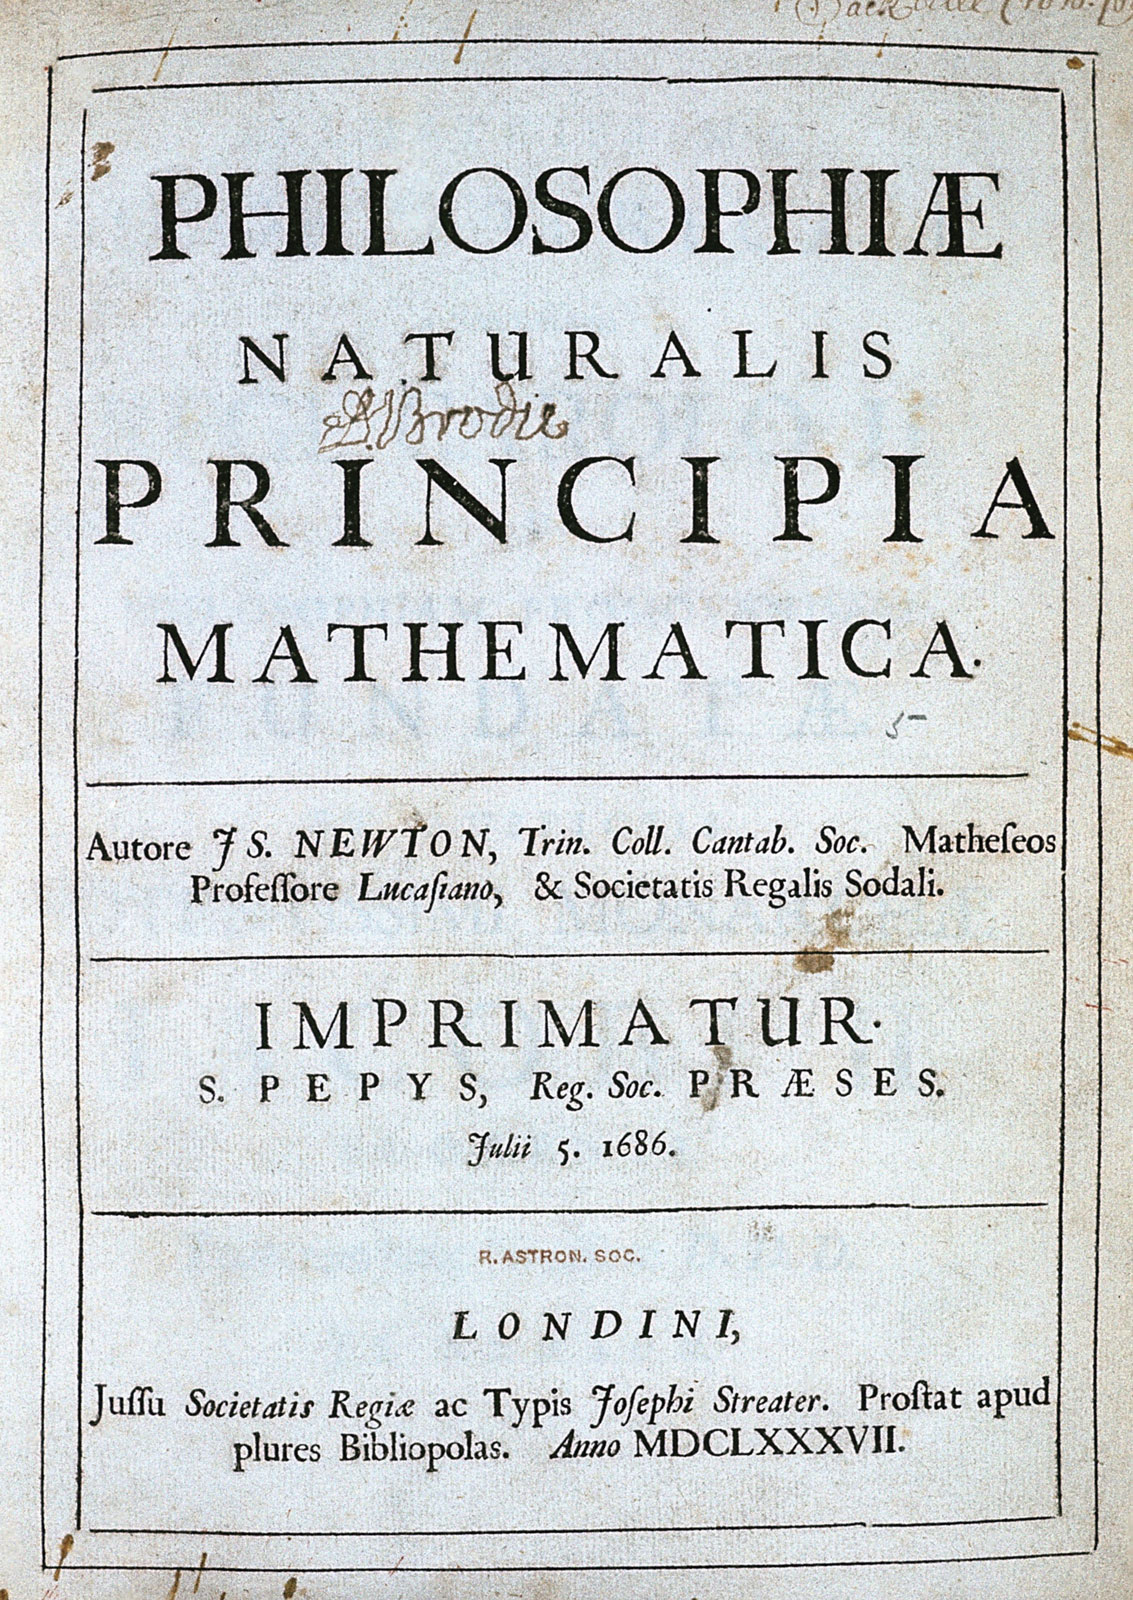
\includegraphics[width=8cm]{nayakn_image1}
    \caption{Sir Isaac Newton's \textit{Principia Mathematica}.}
    \label{fig:1}
\end{figure}

\begin{thebibliography}{2}

\bibitem{} 
Smith, George. “Newton's Philosophiae Naturalis Principia Mathematica.” Stanford Encyclopedia of Philosophy, Stanford University, 20 Dec. 2007, plato.stanford.edu/entries/newton-principia/. 

\bibitem{}
Four Elements: Aristotle, web.lemoyne.edu/~giunta/EA/ARISTOTLEann.html. 

\end{thebibliography}


\newpage

\nnarticleheader{The Fermi Paradox: Are We Alone?}{Matthew Wang, Haverford '21}

\noindent
\textbf{Are We Alone?}

Once in a while, this simple question might jump into your head, creating a wave of mystery and awe. The fact remains that the observable universe is about 93 billion light-years in diameter, yet why haven’t humans found any trace of alien, bacterial, or any carbon-based life forms?

This paradox is what we humans know as The Fermi Paradox. Enrico Fermi had the same question, as the evidence that supports life through the galaxy is indeed optimistic. Billions of Earth-like planets and sun-like stars roam our universe, each has the capability to foster life and more. A closely related question, the Drake Equation, is a systematic means to evaluate the probabilities involved in the existence of alien life. It takes into account the details and intricacies of a galaxy, solar system, and planetary formation. So far, the wait continues for the day humans learn of alien-life. Whether it’s deep inside of Europa (Jupiter’s moon, as shown below), or the Andromeda galaxy; humans still wait.

\renewcommand{\thefigure}{1}
\begin{figure}[h]
  \begin{center}
    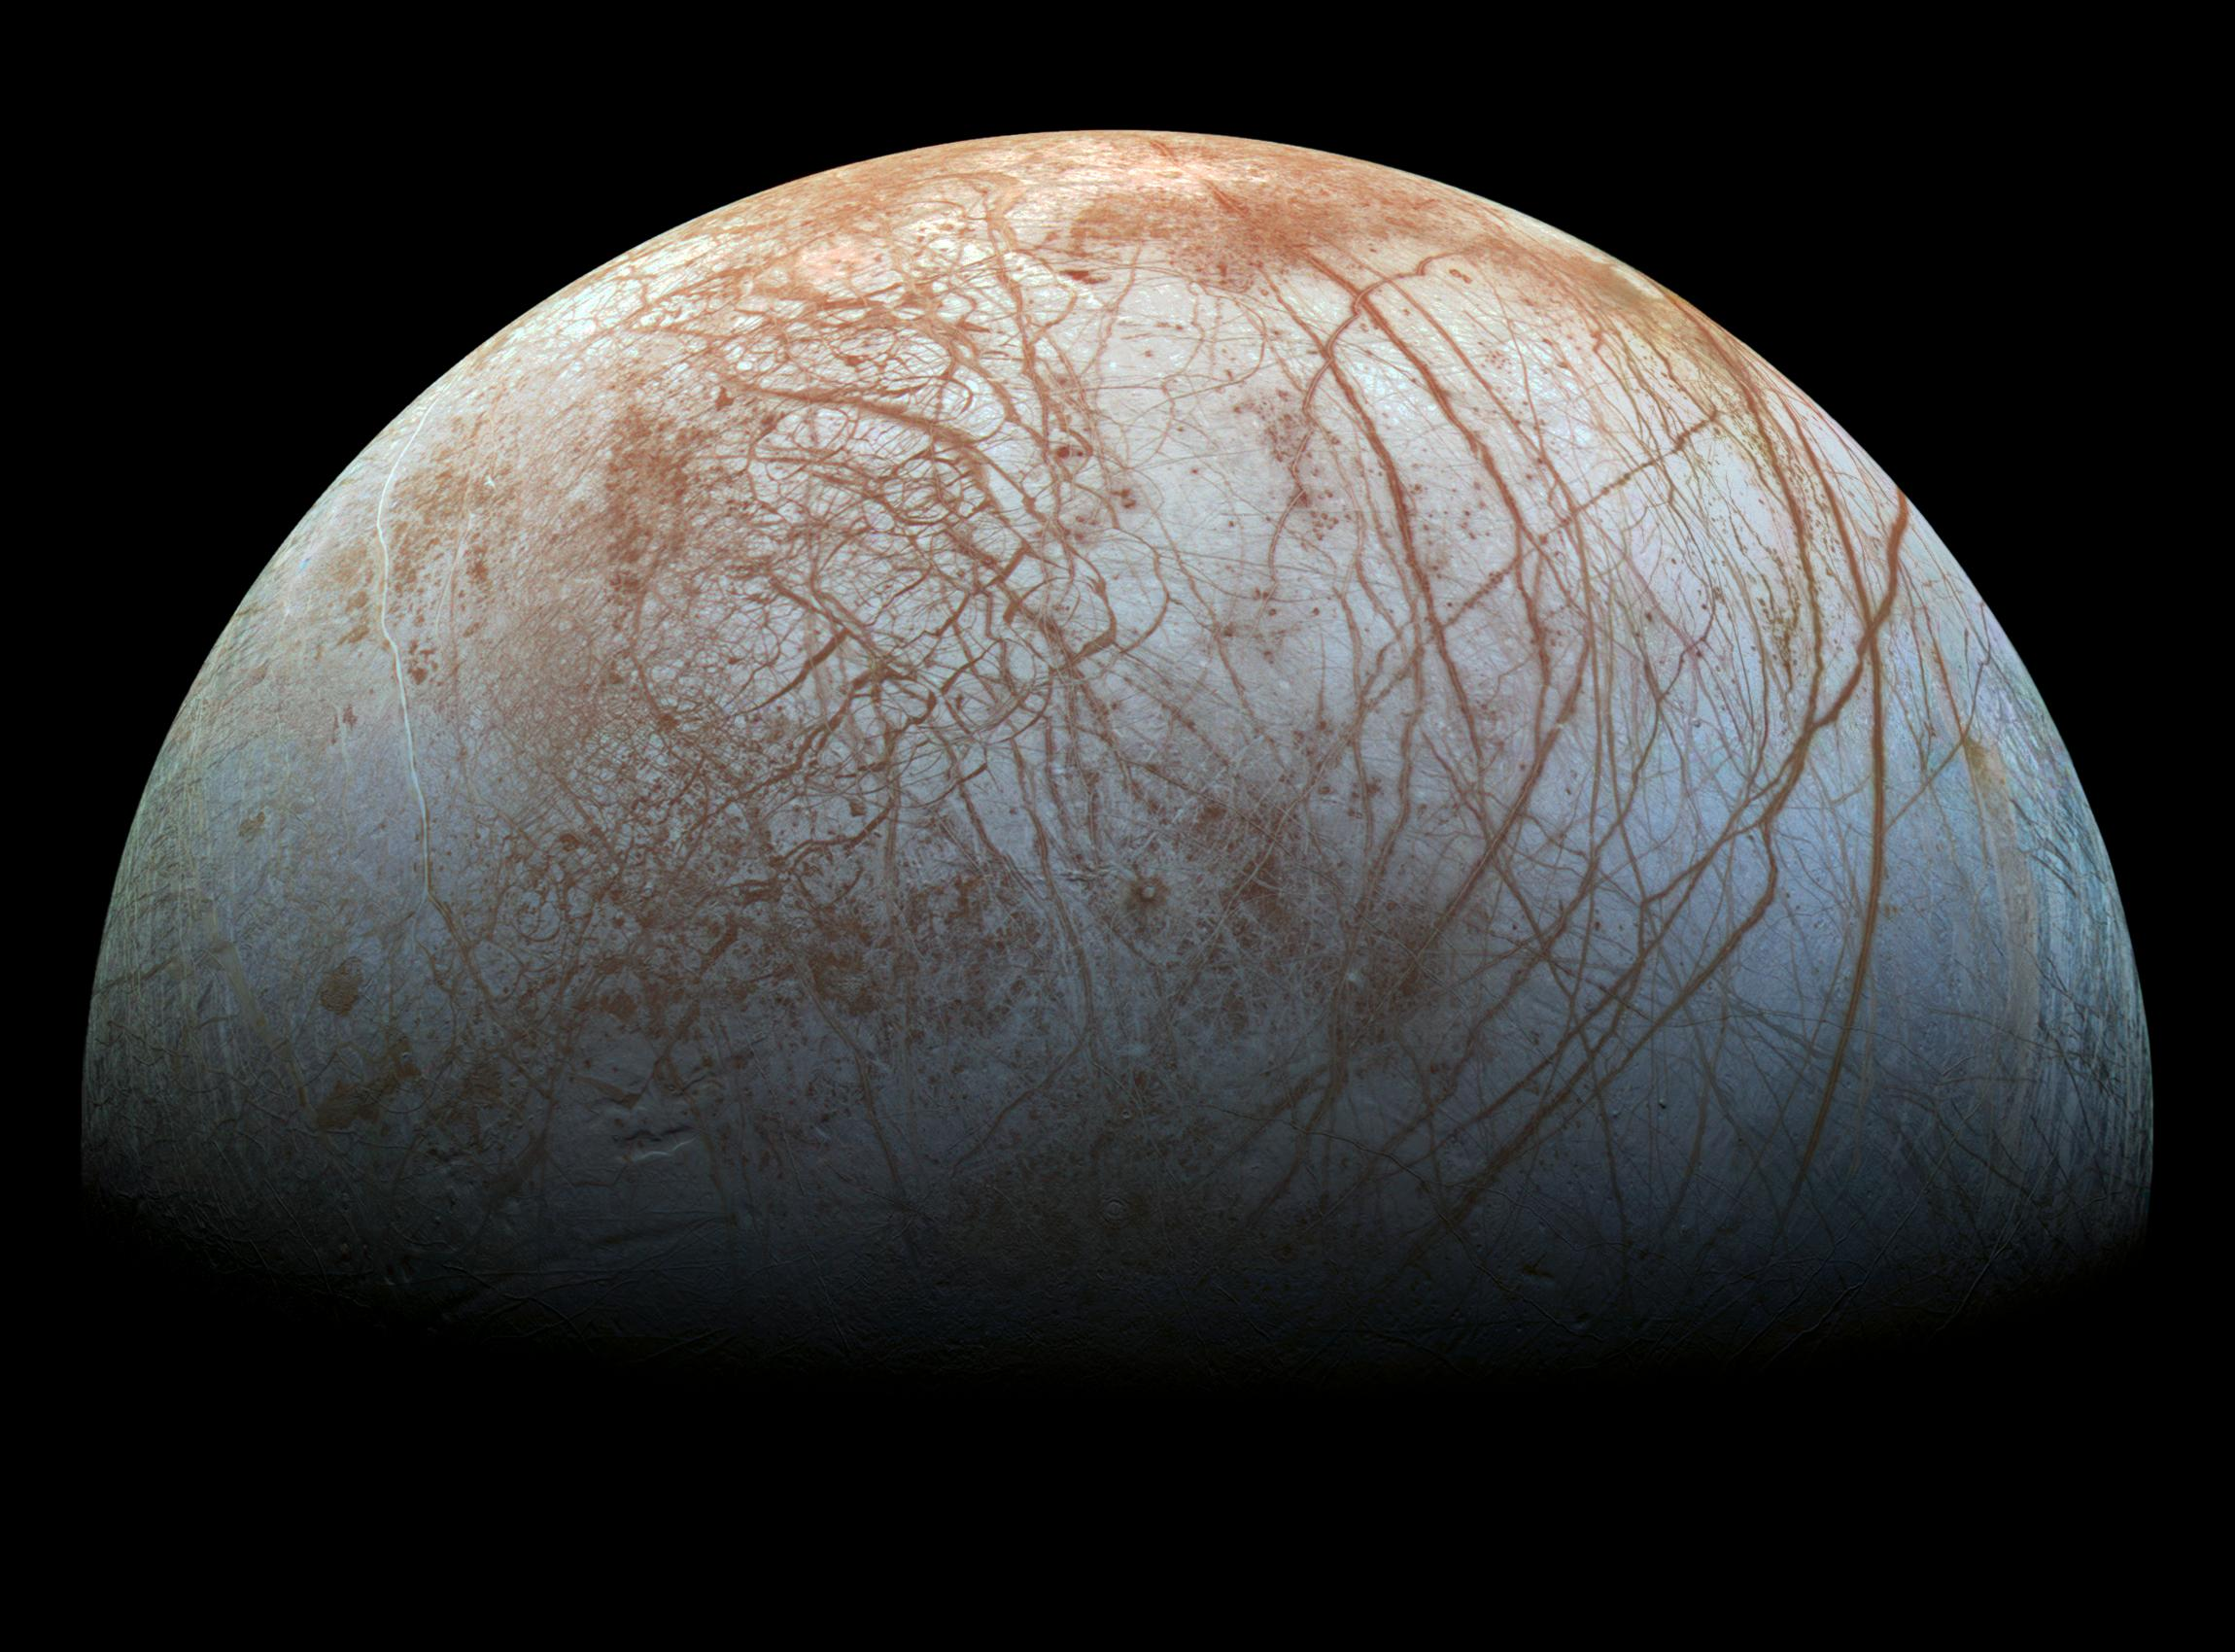
\includegraphics[width=7cm]{wang_image1}
  \end{center}
  \caption{Europa, a moon of Jupiter.}
  \label{fig:1}
\end{figure}

\noindent
\textbf{Possible Explanations}

According to the Kardeshev Scale (a scale that measures a civilization’s level of power, down below), humans have yet to reach stage one. Each level corresponds to a civilization’s power occupancy. The list is as follows: full planetary, solar system, galactical, and universal control. Yet, if an alien civilization were to have advanced through these levels, wouldn’t humans have found signals of life? 

\begin{figure}[htp]
    \centering
    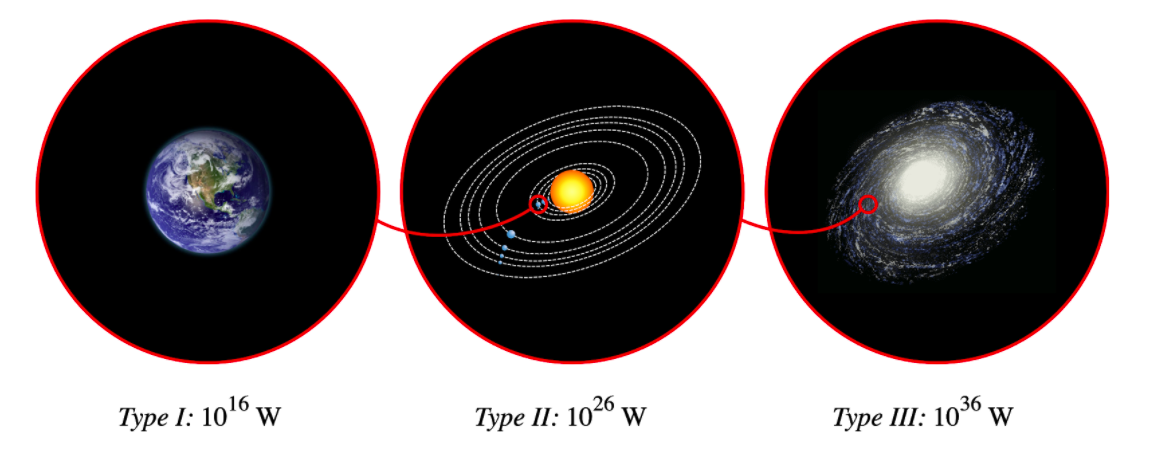
\includegraphics[width=7cm]{wang_image2}
    \caption{The Kardeshec Scale}
    \label{fig:2}
\end{figure}

Known as the Great Filter, there are two widely accepted answers. Life is Rare! Extremely rare. Humans would not have existed if it weren’t for luck. It’s possible that human thought is simply so rare it’s only occurred once. Another answer lies in the fact that intelligent thought always destroys itself. Through technological wars, these intelligent life forms always kill themselves before reaching higher levels of civilization. Now a new question arises. Have we crossed this great filter or have we yet to destroy ourselves? As Nuclear war seems like a possibility, the Anthropocene may be nearing the end. It may be up to us humans to pass this filter.


\newpage

% Begin the math modeling section
\nnwallpaper{2021_Math_Modeling_Page_Border.pdf}
\def\currentTitleWallpaper{2021_Math_Modeling_Title_Page_Border.pdf}

\addcontentsline{toc}{part}{Math Modeling}
\nnimagepage{2021_Math_Modeling_Section_Title.pdf}

%ADD BRIEF SUMMARY OF PROBLEM

\section*{The Problem}

In this year's math modeling contest, ten Fifth and Sixth Formers formed two teams and produced two papers in the 14-hour period. Below is the problem with which they were presented.

	\includegraphics[width=\textwidth]{m3problem}
	
The following two articles include excerpts from each team's submission. From Team 15202, we present an executive summary and a solution to Q1. From Team 15201, we present an executive summary and a solution to Q3.


\newpage

\nnarticleheader{Math Modeling Solution Paper Team 15202}{Nathan Tai '21, Brian Williams '21, Mitav Nayak '22, Jeffrey Yang '22, Bram Shorck '22}

\section*{Executive Summary}
    \indent Many aspects of human life have declined as a result of the pandemic, but one industry which has surged higher than ever in recent weeks is internet connectivity. However, this great fortune of revolutionary communication has been unequally distributed across the country. Low income families continue to struggle to acquire internet access; the consequences of such are even vastly more severe in a remote environment. There is good news, though; past data shows a rapid exponential decrease in the price of data (calculated in megabits per second per United States Dollar) and futuristic connections are being enjoyed by a wider audience than ever before. The trend shows no sign of stopping in the future, and a stable internet connection will soon be a staple like water. But like water, not everyone gets it, and everyone needs different amounts for different things. As the internet becomes more widespread and important, the allocation and distribution methods must adapt and develop complexity to meet the evolving needs of the community. The answer to that question must start with these needs. Before these needs are satisfied, however, the primary focus should be the establishment of its basic resource. Water coverage is great, but it is incomplete, and with internet connection, society has an opportunity to learn from its mistakes. Currently, it is repeating these mistakes with vast swaths of land in digital darkness or stuck with primitively incompatible artifacts which serve as no more than decoration. A perfect model should distribute cellular nodes to cover the entire land, not just the densely populated metro areas. \\
	\indent The first prompt poses a question surrounding the cost of bandwidth; specifically, how this cost will change over the next 10 years. To address the prompt, data for the price of internet and download speed were gathered and leveraged to make calculations and predictions. The models that were created in this prompt—one for the United States and one for the United Kingdom— suggested that the cost per unit of bandwidth have been and will continue to decrease exponentially. The model for the US predicts that price per Mbps will be about 0.70 dollars by the year 2031. \\
	\indent Internet usage requirements based on specific parameters are asked by the second prompt. By creating and defining parameters and values to generate a model that calculates internet consumption rates based on general age ranges, an accurate estimation of internet consumption can be generated for a diverse collection of individuals.\\
	\indent The third prompt requires a pattern of cellular node distribution based on several variables such as population density and income to accurately and effectively serve the internet needs of a region. The model calculates the ideal placement of cellular nodes within subregions, either one larger mid-speed node or four high-speed nodes. For example, Region C from the given data could be given total coverage using 12 high-speed nodes and four mid-speed nodes. The model calculated the most efficient spacing and the needed nodes to handle the peak bandwidth a densely populated area uses. 

 
\section*{The Cost of Connectivity}
	\subsection*{Defining the Question}
	Develop a model to determine the cost per unit of bandwidth in dollars or pounds per Mbps over the next 10 years for consumers in the United States and the United Kingdom.
		
	\subsection*{Assumptions}
	\begin{enumerate}
   \item The entire population of the United States is covered by the data for the United States; the entire population of the United Kingdom is covered by the data for the UK.
   \begin{itemize}
     \item \textbf{Justification}: As long as the data is drawn from a sample size greater than 10 cases while also consisting of less than 10 percent of the population, it can be used to examine statistics.
   \end{itemize}
   \item The price of a monthly internet (given) in the UK remains constant over the year.
   \begin{itemize}
     \item \textbf{Justification}: The given values in D3 did not vary greatly over the course of one year. Calculating an average of the monthly values in a given year was far more efficient than using each monthly value separately.
   \end{itemize}
   \item The potential of technological advancement is unlimited; computers will continue to get more sophisticated and faster while remaining at a constant cost. S, the download speed, is increasing exponentially.
   \begin{itemize}
     \item \textbf{Justification}: The storage space of information in a digital medium has been decreasing exponentially since the invention of computation in addition to processing times. For the purpose of the model, it is assumed that technology will continue this trend into the future.
   \end{itemize}
\end{enumerate}

	\subsection*{Variables}

	\begin{center} \begin{tabular} {|c|c|}
		\hline
		Symbol & Definition \\
		\hline
		$t$ & Time in years\\
		\hline
		$P_D$ & Price in US dollars \\
		\hline
		$P_P$ & Price in British pounds \\
		\hline
		$s$ & Download speed in Megabits per second (Mbps) \\
		\hline
		$P_M$ & Price per Megabit per second (Mbps) \\
		\hline
	\end{tabular} \end{center}


	\subsection*{Developing the Model}
	\subsubsection*{Part I: United States}
%	\noindent \textbf{Part I: United States}

	With data from the NCTA [1] from past years, an exponential regression model was created which could be used to extrapolate the future prices of internet consumption ($P_M$). The data included certain years and the Price per Mbps during that year.

    \begin{center}
    \begin{tabular}{|l|l|}
    \hline
    \multicolumn{2}{|c|}{Price per Mbps ($P_M$) vs time ($t$)} \\ \hline
    Time (years after 2000)     & Price per Mbps ($P_M$)     \\ \hline
    0                           & 28.13                   \\ \hline
    6                           & 9.01                    \\ \hline
    8                           & 9.01                    \\ \hline
    16                          & 0.89                    \\ \hline
    18                          & 0.76                    \\ \hline
    20                          & 0.64                    \\ \hline
    \end{tabular}
    \end{center}
	
	\renewcommand{\thefigure}{1}
    \begin{figure}[htp]
    \centering
    \begin{minipage}{9cm}
    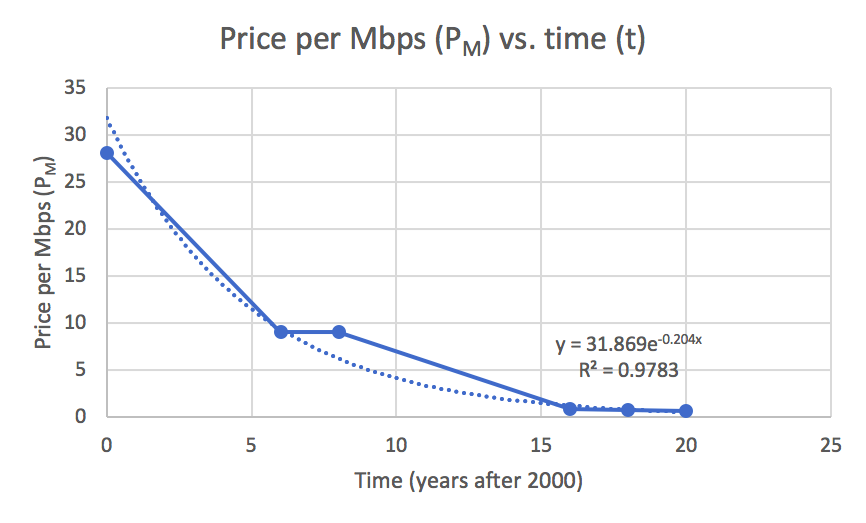
\includegraphics[width=9cm]{modelinga_image1}
    \caption{The model that can be used to predict the cost per unit of bandwidth in dollars per Mbps over the next 10 years. The value of R-squared was 0.9783, demonstrating the effectiveness of the model.}
    \label{fig:1}
    \end{minipage}
    
    \end{figure}
    
    A second data set was also found, with 18 data points, in another study [2] to create a second model, as shown below.
    
    \begin{center}
        
\begin{tabular}{|l|l|l|}
\hline
\multicolumn{3}{|c|}{Price per Mbps ($P_M$) vs time ($t$) — Table 2} \\ \hline
Time (years after 1998)   & Price per Mbps ($P_M$)   & \% decline  \\ \hline
0                         & 1200                  &             \\ \hline
1                         & 800                   & 33          \\ \hline
2                         & 675                   & 16          \\ \hline
3                         & 400                   & 41          \\ \hline
4                         & 200                   & 50          \\ \hline
5                         & 120                   & 40          \\ \hline
6                         & 90                    & 25          \\ \hline
7                         & 75                    & 17          \\ \hline
8                         & 50                    & 33          \\ \hline
9                         & 25                    & 50          \\ \hline
10                        & 12                    & 52          \\ \hline
11                        & 9                     & 25          \\ \hline
12                        & 5                     & 44          \\ \hline
13                        & 3.25                  & 35          \\ \hline
14                        & 2.34                  & 28          \\ \hline
15                        & 1.57                  & 33          \\ \hline
16                        & 0.94                  & 40          \\ \hline
17                        & 0.63                  & 33          \\ \hline
\end{tabular}

    \end{center}
	
	\renewcommand{\thefigure}{2}
	\begin{figure}[htp]
    \centering
    \begin{minipage}{9cm}
    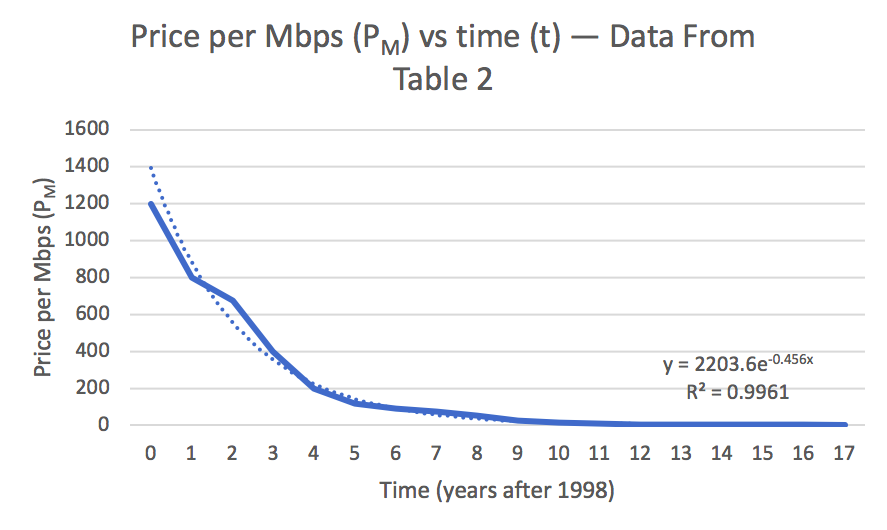
\includegraphics[width=9cm]{modelinga_image2}
    \caption{A second model that shows Price per Mbps vs time.}
    \label{fig:2}
    \end{minipage}
    \end{figure}
	
	While the R-squared value of this model was 0.9961—higher than the R-squared value of the first model—this second model cannot be used to extrapolate over the next 10 years. Still, it was useful in providing supporting evidence that the Price per Mbps decreases exponentially over time.

    Further, D2 provided values of Median Peak Download Speed (Mbps) and Median Monthly Price (\$) for various cities. For five cities, there were values for both 2012 and 2020. For these cities, the Median Monthly Price was divided by the Median Peak Download Speed (Mbps) to calculate the Price per Mbps ($P_M$). The percent change was similar to the percent change calculated in the previous two data sets, furthering the confidence in the model.
	
	
	\begin{center}
\begin{tabular}{|l|l|l|}
\hline
\multicolumn{3}{|c|}{Price per Mbps (PM) in 2012 and 2020} \\ \hline
2012            & 2020            & Percent Change (\%)    \\ \hline
2.082333333     & 0.23196         & 88.86057308            \\ \hline
1.787575758     & 0.188166667     & 89.4736396             \\ \hline
3.120909091     & 0.655172414     & 79.00700101            \\ \hline
2.949           & 0.27495         & 90.67650051            \\ \hline
2.098333333     & 0.4995          & 76.19539317            \\ \hline
\end{tabular}
\end{center}
	
    \subsubsection*{Part II: United Kingdom}
    
    Price data on monthly internet plans for the United Kingdom were provided by data sets in D3. These monthly prices provided in a year were averaged to calculate a singular monthly value that could be used for all months in that given year. This method was used to find the prices for months in years from 2014 to 2019.

    The download speed data was gathered by Akamai from 2010 and 2017. Data gathered by Ookla was not available before 2017, and the source differed from Akamai in its measurement methodology, so it was omitted to maintain data continuity.

    To find the prices from years 2010 through 2013, a linear model was created from the price data based on year.

    \renewcommand{\thefigure}{3}
	\begin{figure}[htp]
    \centering
    \begin{minipage}{9cm}
    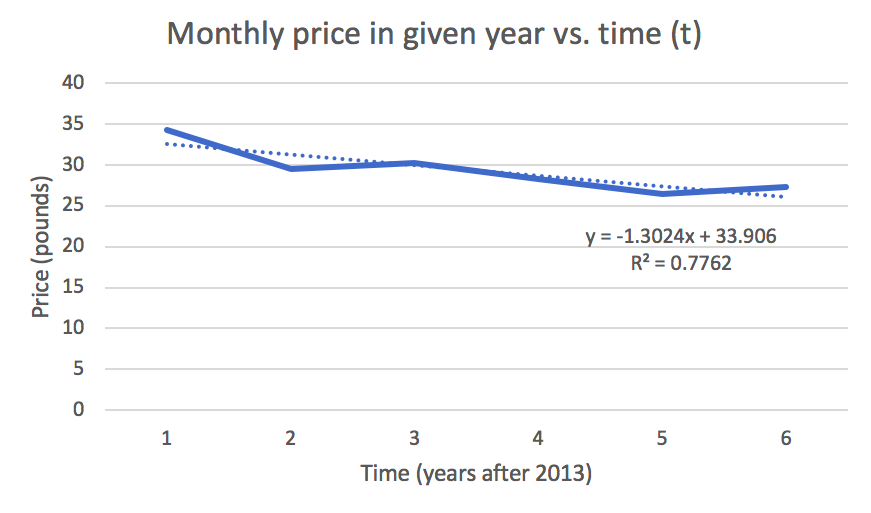
\includegraphics[width=9cm]{modelinga_image3}
    \caption{Monthly internet price (pounds) in UK in the years after 2013.}
    \label{fig:3}
    \end{minipage}
    \end{figure}
    
    This model was used to extrapolate prices from 2010 to 2013. Then, prices from 2010 through 2017 could be divided by the download speed to calculate $P_M$ and create the United Kingdom model.

% Please add the following required packages to your document preamble:
% \usepackage[table,xcdraw]{xcolor}
% If you use beamer only pass "xcolor=table" option, i.e. \documentclass[xcolor=table]{beamer}
\begin{center}
\begin{tabular}{|l|l|}
\hline
\multicolumn{1}{|c|}{Price}   & \multicolumn{1}{c|}{Speed (Mbps)} \\ \hline
{\color[HTML]{4472C4} 37.813} & 3.8                               \\ \hline
{\color[HTML]{4472C4} 36.511} & 4.6                               \\ \hline
{\color[HTML]{4472C4} 35.208} & 5.6                               \\ \hline
{\color[HTML]{4472C4} 33.906} & 7.9                               \\ \hline
34.25                         & 9.9                               \\ \hline
29.5                          & 11.6                              \\ \hline
30.25                         & 14.9                              \\ \hline
28.25                         & 16.9                              \\ \hline
\end{tabular}
\end{center}

\newcommand{\blue}{\color{blue}}
\newcommand{\black}{\color{black}}
The above data table shows the values used for the final UK model. The numbers in \blue blue \black were extrapolated.

    \renewcommand{\thefigure}{4}
    \begin{figure}[htp]
    \centering
    \begin{minipage}{9cm}
    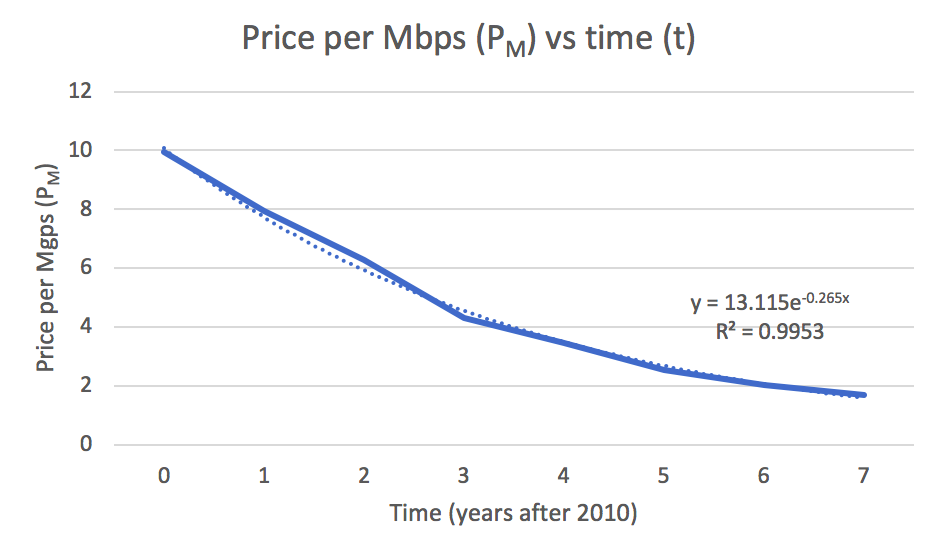
\includegraphics[width=9cm]{modelinga_image4}
    \caption{The final UK model that can be used to to predict the cost per unit of bandwidth in pounds per Mbps over the next 10 years in the UK.}
    \label{fig:4}
    \end{minipage}
    
    \end{figure}
   
   \pagebreak
   \subsection*{Executing the Model}
   \subsubsection*{Part I: United States}
   The model that was built for the United States utilized the equation $y = 31.869e^{-0.204x}$. The independent variable is the number of years after 2000, and the dependent variable is $P_M$. By plugging in values from 20 to 30, the cost per unit of bandwidth per Mbps can be found in any of the next 10 years.
   
   \begin{center}
\begin{tabular}{|c|c|}
\hline
\multicolumn{2}{|c|}{US Model — Value of PM over next 10 years} \\ \hline
x                          & y                                  \\ \hline
20                         & 0.538824023                        \\ \hline
21                         & 0.439390715                        \\ \hline
22                         & 0.358306595                        \\ \hline
23                         & 0.292185545                        \\ \hline
24                         & 0.238266318                        \\ \hline
25                         & 0.194297216                        \\ \hline
26                         & 0.158442069                        \\ \hline
27                         & 0.129203545                        \\ \hline
28                         & 0.105360629                        \\ \hline
29                         & 0.085917629                        \\ \hline
30                         & 0.070062593                        \\ \hline
\end{tabular}
\end{center}
    
    \subsubsection*{Part II: United Kingdom}
    The model built for the UK utilized the equation $y = 13.115e^{-0.265x}$. The independent variable is the number of years after 2010, and the dependent variable is $P_M$. By plugging in values from 10 to 20, the cost per unit of bandwidth per Mbps (monthly) can be found in any of the next 10 years.
    
    \begin{center}
\begin{tabular}{|c|c|}
\hline
\multicolumn{2}{|c|}{UK Model — Value of PM over the next 10 years} \\ \hline
x                            & y                                    \\ \hline
10                           & 0.92659066                           \\ \hline
11                           & 0.71088587                           \\ \hline
12                           & 0.54539587                           \\ \hline
13                           & 0.41843095                           \\ \hline
14                           & 0.32102272                           \\ \hline
15                           & 0.24629054                           \\ \hline
16                           & 0.18895557                           \\ \hline
17                           & 0.14496784                           \\ \hline
18                           & 0.11122019                           \\ \hline
19                           & 0.08532879                           \\ \hline
20                           & 0.06546475                           \\ \hline
\end{tabular}
    \end{center}
    
    

    \subsection*{Results and Discussion}
    \subsubsection*{Strengths and Weaknesses}

    The exponential regression model provides a superior estimate based on past data used to extrapolate into the future. Its simplicity reduces the background effects of minor variables while still allowing them to affect data through past values. The R-squared values of the models are extremely high, suggesting a level of confidence in the model. However, future predictions are seldom accurate and perfect accuracy is impossible to achieve with predictive models.

    The data for the first model comes from 6 data points taken over a course of 20 years, from 2000 to 2020, while the timeframe of the extrapolation has a duration of 10 years. While the time frame seems sufficient, an ideal model would have more data points 

    The data for the second model comes from 8 data points taken over the course of 7 years. In an ideal model, the time frame may need to be lengthened to improve accuracy and decrease variability in the data. There are further limitations to this model because the invention of the internet is relatively recent, and data on internet traffic in its early days is limited.

    \subsubsection*{Sensitivity Analysis}
    Since both of the models model were found by dividing price by download speed, these two parameters can be found in this equation:
    
    $$P_M(t)=\frac{P(t)}{s(t)}$$
    
    It was found that $P_M(t)$ experiences exponential decay as time increases. The data for $P_D(t)$ showed that the price decreased slightly over time. For $P_P(t)$, the model showed that the price was decreasing linearly. $S(t)$, the download speed, generally varies with internet speeds. Since internet speeds have increased dramatically and exponentially over the last 20 years, the finding that $P_M(t)$ decreases exponentially makes mathematical sense. If a parameter—$P(t)$, for example—was to change slightly, it would not have a significant effect on the model. However, if the behavior of $P(t)$ or $s(t)$ in a fundamental way, the model would no longer be accurate.

\pagebreak
\begin{thebibliography}{3}

\bibitem{} 
R. Lake and A. Makori, "The Digital Divide Among Students During COVID-19: Who Has Access? Who Doesn’t?," 16 June 2020. [Online]. Available: https://www.crpe.org/thelens/digital-divide-among-students-during-covid-19-who-
has-access-who-doesnt.

\bibitem{} 
https://www.ncta.com/industry-data

\bibitem{}
https://drpeering.net/white-papers/Internet-Transit-Pricing-Historical-And-Projected.php


\end{thebibliography}


\newpage

\nnarticleheader{Math Modeling Solution Paper Team 15201}{Gary Gao '21, Julius Huang '22, Elijah Lee '22, Adamya Aggarwal '22, Samuel Kohl '22}

\section*{Executive Summary}

	As technology develops, the impetus on governments and companies to provide widely accessible wifi solutions grows higher and higher; in many ways, your access to high-speed internet defines your lifestyle: in fact, many organizations, such as the U.N., define access to the internet as a human right. This reality has only been exacerbated by the COVID-19 pandemic- many students of disadvantaged socioeconomic backgrounds found themselves driving to parking lots and restaurants to learn virtually from a hotspot. Seeing this information, we are presented with the challenge of three problems: firstly, we have to predict pricing trends for different levels of bandwidth over the next ten years; secondly, we are asked to predict a family’s bandwidth needs based on certain characteristics; finally, we will develop a model optimally placing cell towers in three different regions, ensuring adequate coverage for all citizens based on their needs.\\
	\indent For the first problem, we used given and researched data to perform a multi-linear regression. This method will be further discussed later. We tested a couple of hypothetical factors that we think may affect the price of the Internet Plan and yield different results. \\
	\indent In the second problem, we used given data on age demographics and researched data to construct a rudimentary model on finding the bandwidth needs of a single family. This model takes into account age, employment, entertainment preferences.\\ 
	\indent For the third, we equated the given problem to the “maximal covering location problem” (MCLP). From there, we found our solution using the MCLP, and visualized it with a python simulation and data visualization. 

 
\section*{Mobilizing Mobile}
	\subsection*{Problem Redefined}
	Q3 asks us to find an optimal plan to place cell towers in a region and then demonstrate accuracy in the three hypothetical regions provided.
		
	\subsection*{Assumptions}
	\begin{itemize}
	\item Assumption 1: The word “optimal” in the problem means the most households get internet through the fewest cell towers.
	\item Assumption 2: As long as a house is within range of a tower, we consider it to be fully serviced in terms of bandwidth.
	\end{itemize}

	\subsection*{Approaching the Problem}
	We paralleled this problem to the Maximal Covering Location Problem (MCLP), whose objective is to minimize the number of facilities (that each have a fixed radius r that dictates its service area) necessary to cover the population of a set of n nodes.\\
	\indent Let’s define some variables before we begin.
	\begin{center} \begin{tabular} {|c|c|}
		\hline
		Variable & Definition \\
		\hline
		$g_i$ & Bandwidth demand of household i\\
		\hline
		$Y_i$ & Dummy variable representing whether household i is covered by a tower \\
		\hline
		$x_j$ & Dummy variable representing whether a cell tower is on/off (i.e. used or not) \\
		\hline
		$p$ & Budget constraint \\
		\hline
	\end{tabular} \end{center}
	\indent The MCLP can be modeled through a linear program as follows:
	\begin{center}
		Maximize $\sum_{i\in I} g_iY_i$ \\
		Subject to $\sum_{j\in J}x_j \geq Y_i$ and $\sum_{j\in J}x_j \geq p$ \\
		$x_j \in \{0,1\}, Y_i \in \{0,1\}$
	\end{center}
	Basically, we want to maximize the demand (or the number of households covered). A household cannot be covered unless a tower is turned on/used, and we want to fit the number of towers within a constrained budget. Remember, Yi = 1 if household i is covered by at least one facility, and 0 otherwise.

	\subsection*{Applying the MCLP to an Example}
	For an example simulation, we will be using a very simple service area, composed of one region that has 500 nodes (households) in blue. Each household requires a bandwidth of 20 Mbps and each tower can service an unlimited amount of bandwidth and can service at a range of 45 miles. The number of towers ($p$) was capped at 20, and in this random distribution model, the towers served the maximum number of households (56.8\% of the population), as seen in the image below:

\renewcommand{\thefigure}{1}
    \begin{figure}[!htb]
   \begin{minipage}{0.48\textwidth}
     \centering
     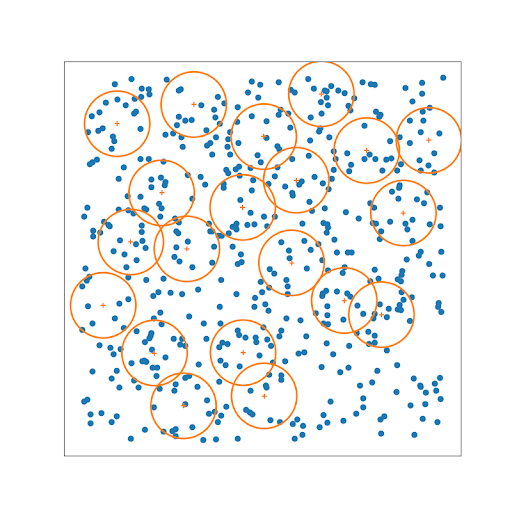
\includegraphics[width=.9\linewidth]{pic1.png}
     
   \end{minipage}\hfill
   \begin{minipage}{0.48\textwidth}
     \centering
     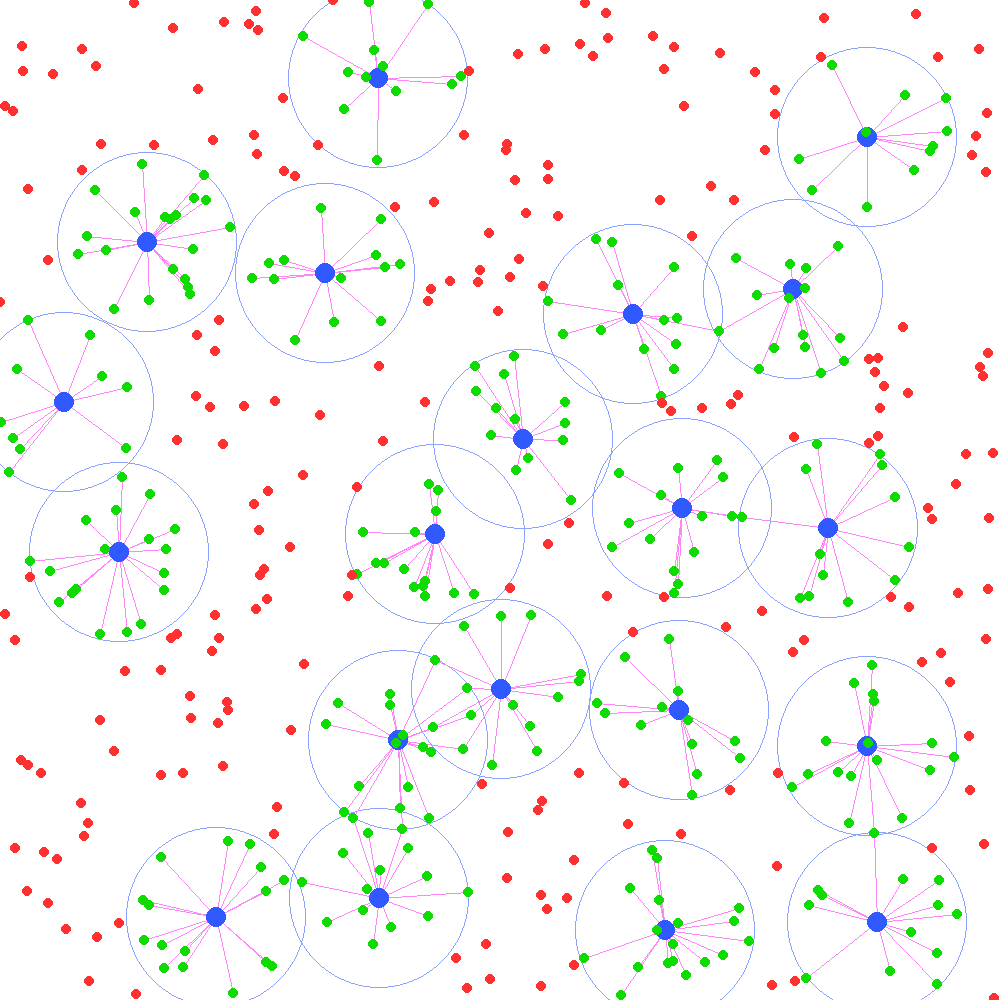
\includegraphics[width=.9\linewidth]{pic2.png}
     
   \end{minipage}
\end{figure}
    
    
    In the below image, we see a representation of the same scenario but with 40 stations, 45 range, 50mbps per household, and 650mbps throughput.
    
    \renewcommand{\thefigure}{1}
    \begin{figure}[!htb]
   \begin{minipage}{0.48\textwidth}
     \centering
     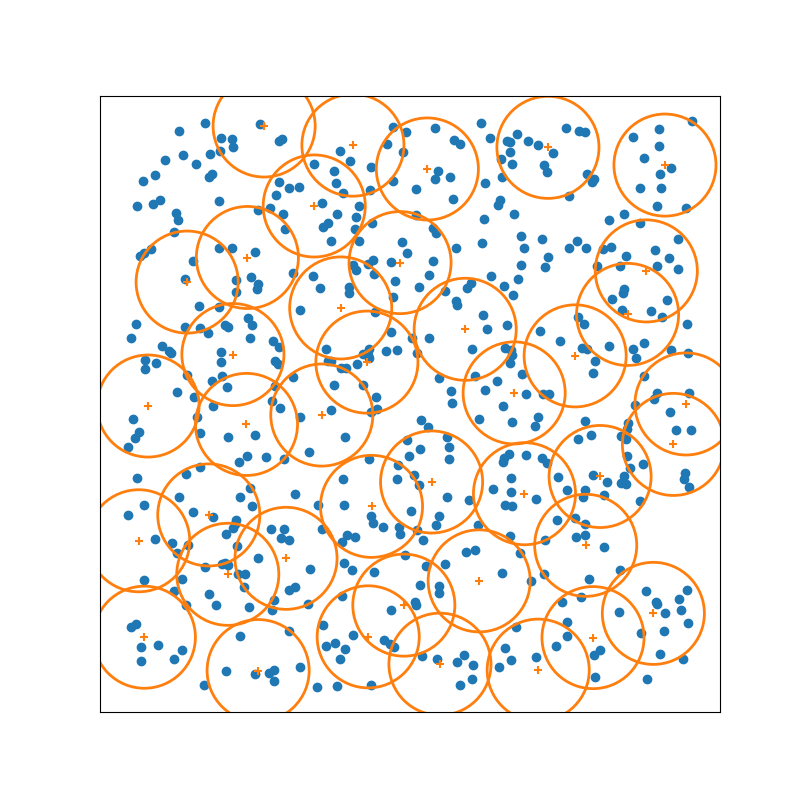
\includegraphics[width=.9\linewidth]{pic3.png}
     
   \end{minipage}\hfill
   \begin{minipage}{0.48\textwidth}
     \centering
     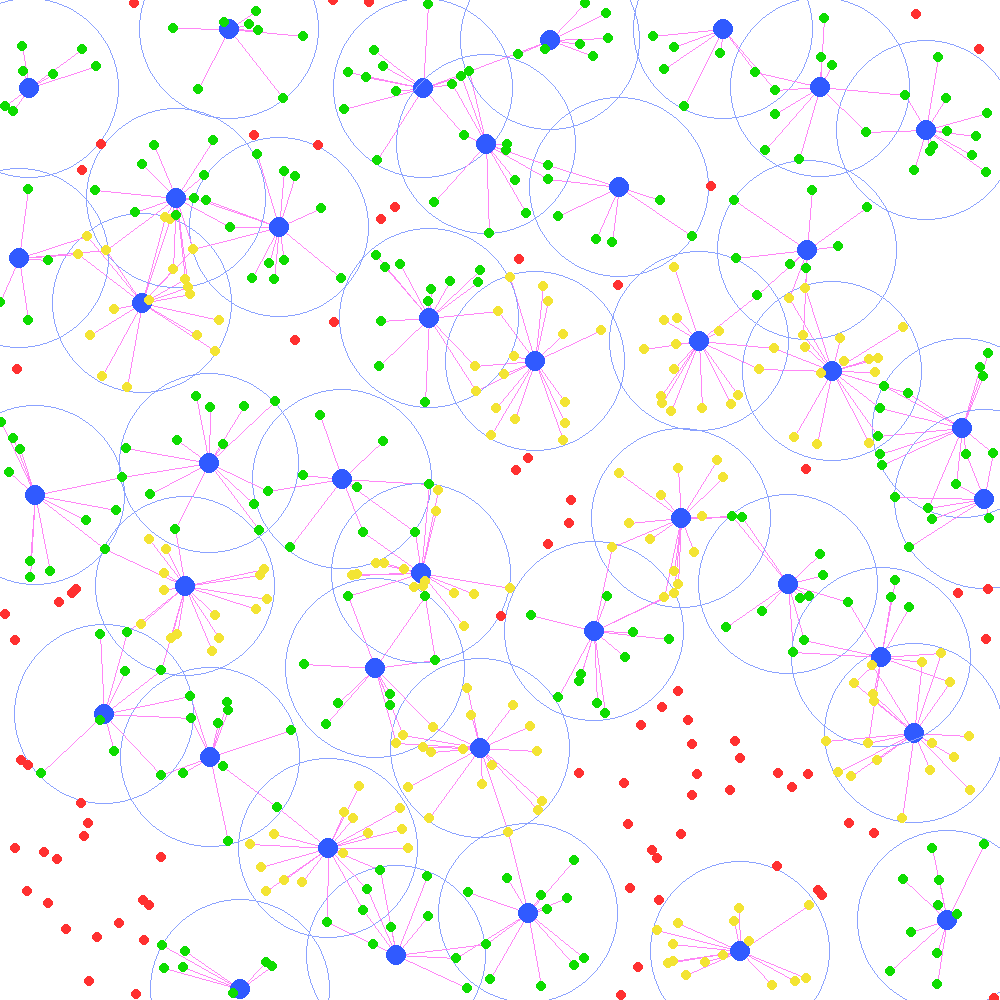
\includegraphics[width=.9\linewidth]{pic4.png}
     
   \end{minipage}
\end{figure}
    

	\subsection*{Simulation Algorithm}
	We created a simulation algorithm to visually represent households that are and aren't covered by a cell tower. Below is the skeleton of the algorithm in pseudocode.
	\begin{enumerate}
	\item For each node i, assign i to a tower if that tower’s range covers that node (note that one node can be assigned to multiple towers).
	\item Add its demand to a variable that represents the tower’s capacity. If a node is covered by two different towers, split its demand evenly and add the halved demand to each tower’s capacity.
	\item Any unserved nodes will be marked red.
	\item Iterate through the towers. If the sum of the demands of each node covered by a certain tower outweighs the tower’s capacity, assign each covered node the color yellow.
	\item Else, assign the nodes the color green.
	\end{enumerate}
	We can see the simulation algorithm results in the images below. In the first image, bandwidth per tower is capped at 200mbps total. 2\% of the nodes are green.
	\begin{figure}[h]
	\centering
	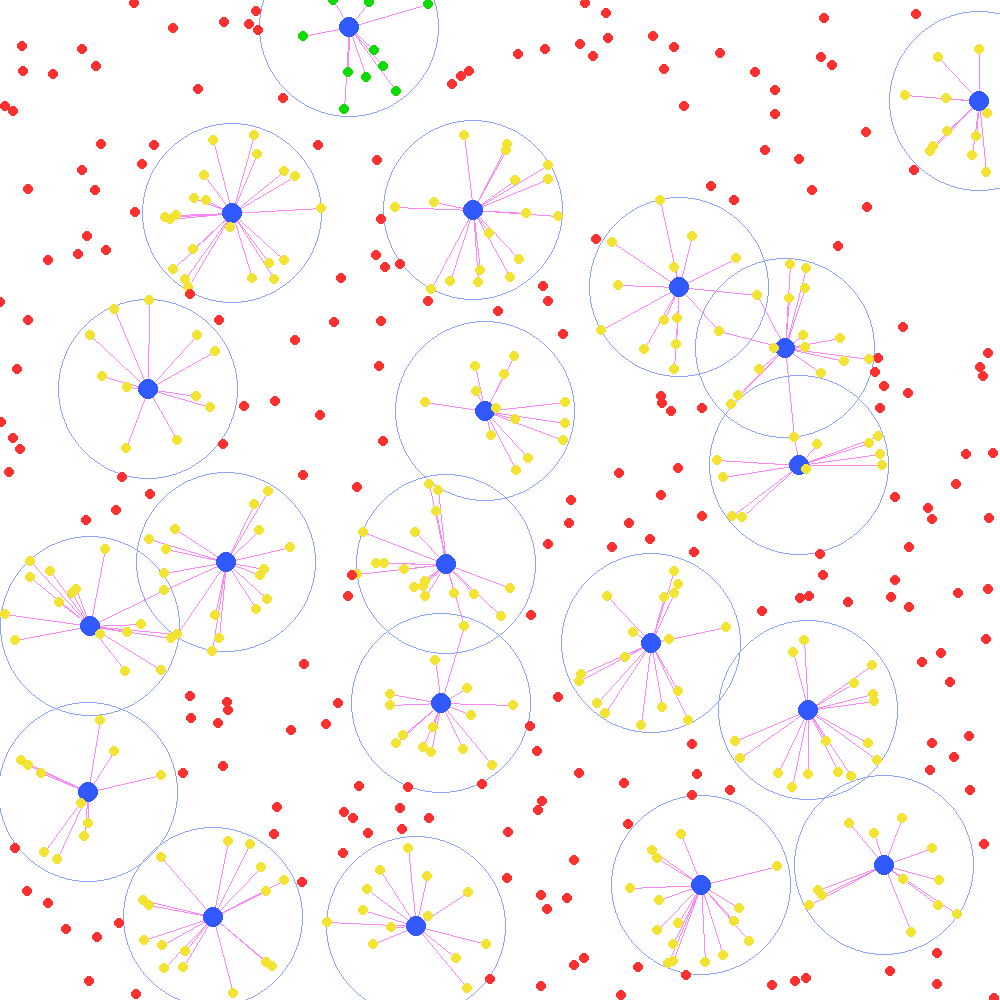
\includegraphics[width=0.5\linewidth]{pic5.png}
	\end{figure}
	
	\subsection*{Flaws and Additional Considerations for Improvements}
	\begin{itemize}
	\item Some houses may need to be in range of more than one tower to be fully serviced given the house’s bandwidth load.
	\item Some towers may be at full capacity and cannot provide bandwidth to any more households. We take this into account in our simulation software, which marks “fully loaded” towers yellow. However, our MCLP solver software does not take this into consideration.
	\item Using the MCLP may not be the most accurate because the solution to this problem, i.e. the minimum number of facilities required for total coverage, may exceed the affordable budget for infrastructure investment. If the budgetary constraint is incorporated in the model, then the objective would be to minimize the maximal service distance S.
	\end{itemize}
	
\section*{Appendix: Code}
	Simulation and MCLP Solver by Elijah Lee.\\
	\indent Note: MCLP solver adapted from https://github.com/cyang-kth/maximum-coverage-location\\
	\indent Note: run \verb|generate_random()| to generate a random distribution and save it for repeatability
	\begin{singlespace}
	\begin{verbatim}
import enum
import pygame
import math
from enum import Enum
 
import numpy as np
from scipy.spatial import distance_matrix
from gurobipy import *
from scipy.spatial import ConvexHull
from shapely.geometry import Polygon, Point
from numpy import random
import random
 
 
#######################################################
 
"""
 
Python implementation of the maximum coverage location problem.
 
The program randomly generates a set of candidate sites, among 
which the K optimal candidates are selected. The optimization 
problem is solved by integer programming. 
 
Author: Can Yang
Date: 2019-11-22
 
MIT License
 
Copyright (c) 2019 Can Yang
 
Permission is hereby granted, free of charge, to any person obtaining a copy
of this software and associated documentation files (the "Software"), to deal
in the Software without restriction, including without limitation the rights
to use, copy, modify, merge, publish, distribute, sublicense, and/or sell
copies of the Software, and to permit persons to whom the Software is
furnished to do so, subject to the following conditions:
 
The above copyright notice and this permission notice shall be included in all
copies or substantial portions of the Software.
 
THE SOFTWARE IS PROVIDED "AS IS", WITHOUT WARRANTY OF ANY KIND, EXPRESS OR
IMPLIED, INCLUDING BUT NOT LIMITED TO THE WARRANTIES OF MERCHANTABILITY,
FITNESS FOR A PARTICULAR PURPOSE AND NONINFRINGEMENT. IN NO EVENT SHALL THE
AUTHORS OR COPYRIGHT HOLDERS BE LIABLE FOR ANY CLAIM, DAMAGES OR OTHER
LIABILITY, WHETHER IN AN ACTION OF CONTRACT, TORT OR OTHERWISE, ARISING FROM,
OUT OF OR IN CONNECTION WITH THE SOFTWARE OR THE USE OR OTHER DEALINGS IN THE
SOFTWARE.
 
"""

def generate_candidate_sites(points,M=100):
    '''
    Generate M candidate sites with the convex hull of a point set
    Input:
        points: a Numpy array with shape of (N,2)
        M: the number of candidate sites to generate
    Return:
        sites: a Numpy array with shape of (M,2)
    '''
    hull = ConvexHull(points)
    polygon_points = points[hull.vertices]
    poly = Polygon(polygon_points)
    min_x, min_y, max_x, max_y = poly.bounds
    sites = []
    while len(sites) < M:
        random_point = Point([random.uniform(min_x, max_x),
                             random.uniform(min_y, max_y)])
        if (random_point.within(poly)):
            sites.append(random_point)
    return np.array([(p.x,p.y) for p in sites])
 
def mclp(points,K,radius,M):
    """
    Solve maximum covering location problem
    Input:
        points: input points, Numpy array in shape of [N,2]
        K: the number of sites to select
        radius: the radius of circle
        M: the number of candidate sites, which will randomly generated inside
        the ConvexHull wrapped by the polygon
    Return:
        opt_sites: locations K optimal sites, Numpy array in shape of [K,2]
        f: the optimal value of the objective function
    """
    print('----- Configurations -----')
    print('  Number of points %g' % points.shape[0])
    print('  K %g' % K)
    print('  Radius %g' % radius)
    print('  M %g' % M)
    import time
    start = time.time()
    sites = generate_candidate_sites(points,M)
    J = sites.shape[0]
    I = points.shape[0]
    D = distance_matrix(points,sites)
    mask1 = D<=radius
    D[mask1]=1
    D[~mask1]=0
    # Build model
    m = Model()
    # Add variables
    x = {}
    y = {}
    for i in range(I):
      y[i] = m.addVar(vtype=GRB.BINARY, name="y%d" % i)
    for j in range(J):
      x[j] = m.addVar(vtype=GRB.BINARY, name="x%d" % j)
 
    m.update()
    # Add constraints
    m.addConstr(quicksum(x[j] for j in range(J)) == K)
 
    for i in range(I):
        m.addConstr(quicksum(x[j] for j in np.where(D[i]==1)[0]) >= y[i])
 
    m.setObjective(quicksum(y[i]for i in range(I)),GRB.MAXIMIZE)
    m.setParam('OutputFlag', 0)
    m.optimize()
    end = time.time()
    print('----- Output -----')
    print('  Running time : %s seconds' % float(end-start))
    print('  Optimal coverage points: %g' % m.objVal)
    
    solution = []
    if m.status == GRB.Status.OPTIMAL:
        for v in m.getVars():
            # print v.varName,v.x
            if v.x==1 and v.varName[0]=="x":
               solution.append(int(v.varName[1:]))
    opt_sites = sites[solution]
    return opt_sites,m.objVal
 
def plot_input(points):
    '''
    Plot the result
    Input:
        points: input points, Numpy array in shape of [N,2]
        opt_sites: locations K optimal sites, Numpy array in shape of [K,2]
        radius: the radius of circle
    '''
    from matplotlib import pyplot as plt
    fig = plt.figure(figsize=(8,8))
    plt.scatter(points[:,0],points[:,1],c='C0')
    ax = plt.gca()
    ax.axis('equal')
   ax.tick_params(axis='both',left=False, top=False, right=False,
                       bottom=False, labelleft=False, labeltop=False,
                       labelright=False, labelbottom=False)
 
def plot_result(points,opt_sites,radius):
    '''
    Plot the result
    Input:
        points: input points, Numpy array in shape of [N,2]
        opt_sites: locations K optimal sites, Numpy array in shape of [K,2]
        radius: the radius of circle
    '''
    from matplotlib import pyplot as plt
    fig = plt.figure(figsize=(8,8))
    plt.scatter(points[:,0],points[:,1],c='C0')
    ax = plt.gca()
    plt.scatter(opt_sites[:,0],opt_sites[:,1],c='C1',marker='+')
    for site in opt_sites:
        circle = plt.Circle(site, radius, color='C1',fill=False,lw=2)
        ax.add_artist(circle)
    ax.axis('equal')
    ax.tick_params(axis='both',left=False, top=False, right=False,
                       bottom=False, labelleft=False, labeltop=False,
                       labelright=False, labelbottom=False)
    fig.show()
    input()
 
#######################################################
 
RESOLUTION = [1000, 1000]
PIXEL_MULTIPLIER = 2
 
TOWER_RANGE = 45
 
PINK = (255, 134, 246)
YELLOW = (243, 228, 51)
BLUE = (48, 90, 255)
RED = (255, 48, 48)
GREEN = (14, 220, 0)
LIGHT_BLUE = (139, 162, 255)
 
status_color = [RED, YELLOW, GREEN]
 
# keep track of marked nodes
visited = []
 
# Setup a class for each node
class Node:
    x = 0
    y = 0
    bandwidth = 0
 
    # for nodes, 0 = red (no service), 1 = orange (bandwidth issues), 2 = green (satisfied)
    # for towers, track demand
    status = -1
    
    def __init__(self, x, y, bandwidth, connection=None):
        self.x = x
        self.y = y
        self.bandwidth = bandwidth
        
        if connection == None:
            connection = []
        self.connection = connection
    
    def set_status(self, status):
        # do not update nodes marked yellow/red
        if self not in visited:
            self.status = status
            visited.append(self)
 
    def __str__(self):
        return "({}, {}) -- {}".format(self.x, self.y, self.bandwidth)
 
    def __repr__(self):
        return "({}, {}) -- {}".format(self.x, self.y, self.bandwidth)
 
nodes = []
towers = []
 
def reset_graph():
    for node in nodes:
        node.connection = []
    for tower in towers:
        tower.connection = []
 
# Connect nodes to their towers
def buildNodeGraph():
    reset_graph()
    for node in nodes:
        for tower in towers:
            if math.sqrt((node.x - tower.x)**2 + (node.y - tower.y)**2) <= TOWER_RANGE:
                tower.connection.append(node)
                node.connection.append(tower)
 
def calcNodeStatus():
    for node in nodes:
        if len(node.connection) == 0:
            node.set_status(0)
        elif len(node.connection) == 1:
            node.connection[0].status += node.bandwidth
        else:
            for tower in node.connection:
                tower.status += node.bandwidth / len(node.connection)
    
    for tower in towers:
        for node in tower.connection:
            node.set_status(1 if tower.status > tower.bandwidth else 2)
 
def score():
    green = 0
    for node in nodes:
        if node.status == 2:
            green += 1
    return green / len(nodes)
 
# Generate random point distribution
def generate_random():
    points = []
    # Region A, 500, 500 miles
    for i in range(0, 500):
        points.append(np.array([500 * random.random(), 500 * random.random()]))
    points = np.array(points)
    np.save("{}/profile.npy".format(os.path.dirname(os.path.abspath(__file__))), points)
 
# generate_random()
 
points = np.load("{}/profile.npy".format(os.path.dirname(os.path.abspath(__file__))))
 
# Starting number of sites to select
K = 40
 
# Service radius of each site
radius = 45
 
# Candidate site size (random sites generated)
M = 100
 
points = np.array(points)
 
# Run mclp 
# opt_sites is the location of optimal sites 
# f is the number of points covered
opt_sites,f = mclp(points,K,radius,M)
 
# Plot the result 
plot_result(points,opt_sites,radius)

 
for point in points:
    nodes.append(Node(point[0], point[1], 50))
for tower in opt_sites:
    towers.append(Node(tower[0], tower[1], 650))
 
# nodes = [Node(30, 20, 100), Node(20, 40, 50), Node(20, 55, 100)]
# towers = [Node(20, 30, 200), Node(20, 60, 200)]
 
buildNodeGraph()
calcNodeStatus()
 
print("SCORE: {}".format(score()))
 
# Initialize pygame
pygame.init()
screen = pygame.display.set_mode(RESOLUTION)
running = True
 
# Main loop
while running:
 
    # Event handling
    for event in pygame.event.get():
        if event.type == pygame.QUIT:
            running = False
 
    # Fill the background with white
    screen.fill((255, 255, 255))
 
    # Draw nodes
    for tower in towers:
    	for node in tower.connection:
    	pygame.draw.line(screen, PINK, (tower.x * PIXEL_MULTIPLIER, tower.y * PIXEL_MULTIPLIER), 
(node.x * PIXEL_MULTIPLIER, node.y * PIXEL_MULTIPLIER))
    pygame.draw.circle(screen, BLUE, (tower.x * PIXEL_MULTIPLIER, tower.y * PIXEL_MULTIPLIER), 10.0)
    pygame.draw.circle(screen, LIGHT_BLUE, (tower.x * PIXEL_MULTIPLIER, tower.y * 
PIXEL_MULTIPLIER), TOWER_RANGE * PIXEL_MULTIPLIER, 1)
    for node in nodes:
        pygame.draw.circle(screen, status_color[node.status], (node.x * PIXEL_MULTIPLIER, node.y 
* PIXEL_MULTIPLIER), 5.0)
    
    # Render
    pygame.display.flip()
 
pygame.quit()
 
	\end{verbatim}
	\end{singlespace}

\begin{thebibliography}{2}

\bibitem{} 
Measuring broadband america. (2021, February 12). Retrieved March 01, 2021, from https://www.fcc.gov/general/measuring-broadband-america

\bibitem{}
Markgraf, B. (2016, October 26). How far can a cell tower be for a cellphone to pick up the
signal? Retrieved March 02, 2021, from https://smallbusiness.chron.com/far-can-cell-
tower-cellphone-pick-up-signal-32124.html

\bibitem{}
Berry, J. J. (2020, August 27). COVID-19 exposes why access to the internet is a human
right. Retrieved March 02, 2021, from http://www.openglobalrights.org/covid-19-exposes-why-access-to-internet-is-human-right/.

\bibitem{}
Dvorak, Petula. “Perspective | When &#39;Back to School&#39; Means a Parking Lot and the Hunt for a
WiFi Signal.” The Washington Post, WP Company, 27 Aug. 2020,
www.washingtonpost.com/local/when-back-to-school-means-a-parking-lot-and-the-hunt-for-a-
wifi-signal/2020/08/27/0f785d5a-e873-11ea-970a-64c73a1c2392\_story.html.

\bibitem{}
Chung, C. (1986). Recent Applications of the Maximal Covering Location Planning
(M.C.L.P.) Model. Retrieved March 1, 2021, from https://www.jstor.org/stable/2581958

\bibitem{}
https://www.youtube.com/watch?v=i2Xy3VSkGRs

\bibitem{}
https://www.youtube.com/watch?v=sA8ItKmdwjM

\bibitem{}
Zarandi, M., Davari, S., &amp; Sisakht, S. (2011, November 19). The large scale maximal covering location problem. Retrieved March 02, 2021, from
https://www.sciencedirect.com/science/article/pii/S1026309811002100#s000040

\bibitem{} 
Snyder, S., &amp; Haight, R. (2016). Application of the Maximal Covering Location Problem
to Habitat Reserve Site Selection: A Review. Retrieved March 1, 2021, from
https://www.fs.fed.us/nrs/pubs/jrnl/2016/nrs\_2016\_snyder\_001.pdf

\bibitem{}
Goldstein, R. (2014, July 25). Duality in Linear Programming. Retrieved March 1, 2021,
from http://web.mit.edu/15.053/www/AMP-Chapter-04.pdf

\bibitem{}
Rodriguez, F., Blum, C., Lozano, M., &amp; Garcia-Martinez, C. (2012, April). Iterated Greedy
Algorithms for the Maximal Covering Location Problem. Retrieved March 1, 2021, from
https://www.researchgate.net/publication/265311031\_Iterated\_Greedy\_Algorithms\_for\_the\_Maximal\_Covering\_Location\_Problem


\end{thebibliography}


\newpage

% Begin the mathematical brainteasers section
\nnwallpaper{2021_Math_Brainteasers_Page_Border.pdf}
\def\currentTitleWallpaper{2021_Math_Brainteasers_Title_Page_Border.pdf}

\addcontentsline{toc}{part}{Mathematical Brainteasers}
\nnimagepage{2021_Math_Brainteasers_Section_Title.pdf}

\noindent
\textbf{Introduction}

The following riddle was taken from \emph{How to Solve It}, a famous book describing the mathematical method by George Pólya. It was published in 1945, and it describes four steps one can take when problem solving:

\begin{enumerate}
   \item Understanding the Problem
   \begin{itemize}
     \item Here, you may have to identify the unknown, conditions, and data, draw a figure, and introduce notation.
   \end{itemize}
   \item Devising a Plan
   \begin{itemize}
     \item Next, you examine a connection between the data and the unknown. You may consider a similar problem to devise your plan.
   \end{itemize}
   \item Carrying Out the Plan
   \begin{itemize}
     \item The next step is to carry out your plan, checking each step as you work through the problem.
   \end{itemize}
   \item Looking Back
   \begin{itemize}
     \item Finally, check your final answer. You may consider using a different method to derive the same result.
   \end{itemize}
\end{enumerate}

\noindent
We will now use Polya’s steps on a classic brainteaser.

\noindent
\textbf{The Problem}

A bear, starting from the point \emph{P}, walked one mile due south. Then he changed direction and walked one mile due east. Then he turned again to the left and walked one mile due north, and arrived exactly at the point \emph{P} he started from. What was the color of the bear?

\noindent
\textbf{The Explanation}

After looking at this problem, we may be initially confused. Firstly, how can a bear walk one mile south, one mile east, and one mile north, and end up at the same point he started? Secondly, how does this pertain to the color of the bear? Let’s break the problem down into the four steps.

\begin{enumerate}
   \item Understanding the Problem
  
   While the first question posed will be important in the solution, it is not the unknown. Rather, the unknown is the color of the bear. The bear’s travel and directions traveled are data, not the unknown.
   
   To understand the problem, we can also draw a figure.
   
   %figure

   \item Devising a Plan
   
   If we have seen a similar problem we may consider that. If not, we can try to connect the data to the unknown. We can pose the following questions:
   
   \begin{itemize}
     \item Where do bears live? What are some colors bears may be?
     \item Where on the earth may a bear be able to walk south, east, and north, and end up at the same spot?
   \end{itemize}
   
   After some thought, we realize that the solution may pertain to a specific location on the earth, since the color of a bear varies depending on its location. Also, the earth is spherical, so our figure would look quite different if we were at some locations on the earth. Our plan may be to draw more figures, each at different points on the earth.
   
   \item Carrying Out the Plan
   
   %figure
   %figure
   %figure
   
   Based on our North Pole figure, we have found where it may be possible for the bear to end up at the same point. We know that bears at the North Pole are white, and this is our answer to the riddle.

   
   \item Looking Back
   
   We can check our figure again. If we assume the globe is a perfect sphere, and the bear moves due south, due east, and due north, it will indeed end at the same place it began: the North Pole.
   
\end{enumerate}

\pagebreak
\begin{thebibliography}{1}

\bibitem{} 
Polya, George. How to Solve It. Princeton University Pres, 2009.

\end{thebibliography}


\newpage

\nnarticleheader{The Missing Dollar Problem}{Adamya Aggarwal, Haverford '22}


\section*{The Problem}
Three travelers register at a hotel and are told that their rooms will cost \$10 each so they pay \$30. Later the clerk realizes that he made a mistake and should have only charged them \$25. He gives a bellboy \$5 to return to them but the bellboy is dishonest and gives them each only \$1, keeping \$2 for himself as a tip. So the men actually spent \$27 and the bellboy kept \$2. What happened to the other dollar of the original \$30?

\section*{The Explanation}
This classic mathematical fallacy tries to trick you by bombarding you with numbers and forcing you to apply a nonsensical equation to make you lose sight of the true answer. If we do our bookkeeping correctly, we see that there is no missing dollar. 

The register has \$25. The total refund was \$5. Of that refund, \$3 went to the guests, and \$2 went to the bellboy. So 25 + 3 + 2 = 30. There doesn’t appear to be a missing dollar. So where is the confusion?

Let’s organize the information in a series of equations:

\vspace{-5mm}

\begin{align*}
    10 + 10 + 10 &= 30 && \text{\$30 is the initial bill} \\
    \midrule
    10 + 10 + 10 &= 25 + 5 && \parbox[t]{5cm}{
          \$25 is the actual bill and \$5 is the refund} \\
    \midrule
    10 + 10 + 10 &= 25 + 3 + 2 && \parbox[t]{5cm}{
          \$3 is how much the bellboy gives back to the guests and \$2 is how much he keeps for himself} \\
    \midrule
    9 + 9 + 9 &= 25 + 2 && \parbox[t]{5cm}{
            Subtracting the \$3 from both sides, we see each guest paid \$9}
\end{align*}

In the last step lies the confusion. The riddle forces you to draw up the equation
\begin{equation*}
    9 + 9 + 9 + 2 = 29 \neq 30
\end{equation*}

But this is simply the wrong equation. Note that the \$9 that each guest pays \textit{includes} the bellboy’s \$2 tip, and there is no reason to add it again. It should be $9 + 9 + 9 = 25 + 2$ because effectively, the guests are paying \$9 each, \$25 to the hotel and \$2 to the bellboy. If we just add back the \$3 that was refunded to the guests, we arrive at a grand total of \$30. There is no missing dollar.

\vspace{5mm}

\textit{An approximate answer to the right question is worth a great deal more than a precise answer to the wrong question}
\begin{flushright}
       John Tukey
\end{flushright}
 


\newpage

\nnwallpaper{2021_Intro_Section_Page_Border.pdf}

\begin{figure}[H]
    \centering
    \vspace*{50pt}
    \includegraphics[scale=1.25]{newtons_notebook_fibonacci_spiral.png}
    \vspace*{25pt}
\end{figure}

    This issue of the \textit{Notebook} included submissions from our own students and faculty. Also added in this issue were two new sections—Math Modeling and Mathematical Brainteasers—containing more complex articles with advanced arguments. The \textit{Notebook} team hopes that the increasing diversity of this journal inspires its readers to pursue STEM with unremitting fervor and renewed dedication. 

\begin{quotation}
\textit{We are at the very beginning of time for the human race. It is not unreasonable that we grapple with problems. But there are tens of thousands of years in the future. Our responsibility is to do what we can, learn what we can, improve the solutions, and pass them on.}
	\begin{flushright}
$\sim$Richard P. Feynman
	\end{flushright}
\end{quotation}

\begin{center}
If you are interested in contributing to the 2021-2022 edition of \textit{Newton’s Notebook},\\ 
please contact Mitav Nayak, Editor for Issue VI.
\end{center}

% v COMMENT THIS OUT BEFORE SENDING THE FINAL VERSION TO PRINT, THEY DON'T WANT THE COVERS
%\newpage
%\nnimagepage{2021_Back_Cover.pdf}

\end{document}
